\documentclass[a4paper, fleqn]{article}
\usepackage[margin=0.5in]{geometry} % page layout
\usepackage{amsmath,amssymb,amsthm} % maths packages
\usepackage{tikz-cd} % commutative diagrams
\usepackage[colorlinks, linkcolor=black, urlcolor=black, citecolor=black]{hyperref} % hyperreferences with black links
\usepackage{graphicx} % graphics
\usepackage{multicol} % multiple columns
\usepackage[none]{hyphenat}  % Prevent hyphenation
\usepackage{microtype} % Improves spacing

\setlength{\parindent}{0pt} % Set the indent for new paragraphs to 0
\setlength{\mathindent}{0pt} % Set the indent for equations to 0

\tolerance=1000
\emergencystretch=\maxdimen
\hyphenpenalty=1000
\hbadness=10000

% Set up Diagram Paths
\graphicspath{{../Graphs}}

% Theorem environments
\theoremstyle{plain}
\newtheorem{theorem}{Theorem}[section]
\newtheorem{proposition}[theorem]{Proposition}
\newtheorem{lemma}[theorem]{Lemma}
\newtheorem{corollary}[theorem]{Corollary}
\newtheorem{claim}[theorem]{Claim}
\newtheorem{conjecture}{Conjecture}
\theoremstyle{definition}
\newtheorem{remark}[theorem]{Remark}
\newtheorem{definition}[theorem]{Definition}
\newtheorem{example}[theorem]{Example}

\RequirePackage{etoolbox}
\AtEndEnvironment{remark}{\hfill$\lozenge$}
\AtEndEnvironment{example}{\hfill$\lozenge$}

% Auxiliary commands
\DeclareMathSymbol{:}{\mathpunct}{operators}{"3A}%semicolon spaces
\RequirePackage{xspace}
\def\mat#1{\ensuremath{#1}\xspace}
\def\dmat#1#2{\gdef#1{\mat{#2}}}
\def\csdmat#1#2{\csdef{#1}{\mat{#2}}}

% Operators. Usage: \GL
\def\oper#1{\csdmat{#1}{\operatorname{#1}}}
\forcsvlist\oper{GL,SL,deg,Hom,End,Vect,Mod,Rep,Ker,Im,Id}

% Mathbb Letters. Usage: \bA
\def\defbb#1{\csdmat{b#1}{\mathbb{#1}}}
\forcsvlist\defbb{A,B,C,D,E,F,G,H,I,J,K,L,M,N,O,P,Q,R,S,T,U,V,W,X,Y,Z}
\RequirePackage{bbm}
\dmat\bk{\mathbbm k}

% Mathcal Letters. Usage: \cA
\def\defcal#1{\csdmat{c#1}{\mathcal{#1}}}
\forcsvlist\defcal{A,B,C,D,E,F,G,H,I,J,K,L,M,N,O,P,Q,R,S,T,U,V,W,X,Y,Z}

% Greek letters
\dmat\al\alpha
\dmat\be\beta
\dmat\ga\gamma
\dmat\de\delta
\dmat\la\lambda
\dmat\ta\tau
\dmat\hi\chi
\dmat\eps\varepsilon
\dmat\vi\phi
\dmat\te\theta
\dmat\ksi\xi
\dmat\si\sigma
\dmat\om\omega
\dmat\Ga\Gamma
\dmat\La\Lambda

% Structures
\def\set#1{\left\{#1\right\}}
\def\sets#1#2{\left\{\left.#1\ \right\vert#2\right\}}
\def\rbr#1{\left(#1\right)}
\def\ang#1{\left\langle#1\right\rangle}
\def\n#1{\left\lvert#1\right\rvert}
\def\nn#1{\left\lVert#1\right\rVert}
\def\eq#1{\begin{equation}#1\end{equation}}
\def\ov#1#2{{\substack{#1\\#2}}} % #1 over #2

% Symbols
\def\mto{\mapsto}
\def\emb{\hookrightarrow}
\def\es{\emptyset}
\def\bs{\backslash}
 % file with useful abbreviations

\begin{document}

\title{\bf\Huge Concerning the Stability \\ of \\ Complex Time Steppers}
\author{\Large Cian J. Duggan}
\date{\today}

\maketitle
\thispagestyle{empty}
\newpage

\tableofcontents
\thispagestyle{empty}
\newpage
\setcounter{page}{1}

\newpage
\section{Introduction}
\par A paper by Lloyd N. Trefethen~\cite{trefethen_definition} offers two definitions of numerical analysis:
\begin{quote}
    \textit{The study of rounding errors.}
\end{quote}
\begin{quote}
    \textit{The study of algorithms for the problems of continuous mathematics.}
\end{quote}

\par Trefethen argues that the first definition, though an accurate summation of the field's history, does not serve to entice the curious to explore the field. He proposes the second as a more compelling definition, one that emphasises the field's role in solving real-world problems, and inspires curiosity.

\par He offers an optimistic view of the field, one that is not bogged down by the minutiae of rounding errors, but rather one that is focused on the algorithms that make numerical analysis possible. More to ground, the majoirity of numerical analysis is concerned with the speed of convergence and minimization of error.

Through my work on this paper, I have honed my own definition:
\begin{quote}
	\textit{Numerical analysis is the field which attempts to straddle the gaps between the discrete and the continuous.}
\end{quote}

In this paper we will take a look at the stability of various numerical methods when applied to problems of differential calculus.\\
In particular, we wish to:
\begin{itemize}
	\item[$\cdot$] Introduce key terminology and concepts in the field of numerical analysis.
	\item[$\cdot$] Establish the Exponential Decay Problem as the toy problem for analysis.
	\item[$\cdot$] Define stability, and its associated concepts, in the context of numerical analysis.
	\item[$\cdot$] Establish the concept of Complex time steps for numerical methods.
	\item[$\cdot$] Develop a framework for the analysis of the stability of numerical methods.
	\item[$\cdot$] Apply this framework to particular numerical methods.
	\item[$\cdot$] Expand upon the results of this to contrast the stability regions for Real and Complex time steps.
	\item[$\cdot$] MORE?
\end{itemize}

\newpage
\section{Definitions and Concepts}

\subsection{Numerical Methods}
\par \term{Numerical methods} are techniques used to approximate solutions to problems that cannot be solved exactly.\\
Numerical methods are prevalent when working with problems of differential calculus in a computational context, where many problems do not have closed-form solutions.\\
A numerical method can be interpreted as an alogorithm; a series of steps that can be followed to approximate a solution.\\
Many numerical methods exist, each with their own properties and tradeoffs.\\
In this respect, different methods may be more or less suitable for different problems.\\
Core to understanding which to use for a particular problem are the concepts of \term{error} and \term{stability}.\\
Before discussing these properties, however, we must understand how a numerical method works.\\
The basis of many numerical methods is the concept of a \term{time step}.

\subsection{Time Steps}
Let's take a step back to when we first studied derivatives.\\
\term{Newton's Difference Quotient} should be familiar: 
$f'(x) = \Lim{h \to 0} \frac{f(x+h) - f(x)}{h}$

\par Viewing Newton's Difference Quotient in the context of numerical methods, we call $h$ a \term{time step}.\\
Due to computational constraints, we cannot take $h$ to be infinitesimal. (A computer's memory is as small as it is big)\\
Instead, we take $h$ to be a small, finite number.\\
This defines the concept of a \term{step size}.\\

\par For numerical methods, we use $y(t)$ to denote the solution to a differential equation at time $t$.\\
We approximate $y'(t)$ by $\frac{y(t+h) - y(t)}{h}$ using Newton's Difference Quotient.\\
Note this is an approximation because we have dropped the limit; $h$ is not infinitesimal.\\
This gives $y(t + h) \approx y(t) + h y'(t)$; a first-order approximation of $y$ a small time step $h$ in the future.\\
For a numerical method we say $y(t + h) = y(t) + h y'(t)$ 

\subsection{Error}
\par In numerical analysis, \term{error} is the difference between the numerical solution and the exact solution to a problem.\\
Error can be caused by many factors, such as the choice of numerical method, the choice of time step, or the precision of the computer.\\
Error can be classified into two categories: truncation error and rounding error.\\
\term{Truncation Error} is the error introduced by approximating a problem, such as using a finite time step.\\
\term{Rounding Error} is the error introduced by the finite precision of a computer.\\
Error is a crucial concept in numerical analysis, as it determines the accuracy of a numerical method.\\
Any error mentioned in this document refers to the truncation error; we won't be looking at how comupters run these calculations and the rounding errors that come with it.

\subsection{Stability}
\par In numerical analysis, a method is said to be \term{stable} if small deviations in the input do not lead to large perturbtions in the output.
In the context of differential equations, a method is said to be stable if the solution does not grow to be unbounded as the number of time steps increases. (This, of course, only applies if the exact solution is bounded. We will restrict ourselves to this with our analysis.)

\par When solving differential equations numerically, the choice of time step is crucial.
If the step size is too large, the solution may become unstable; the numerical solution will diverge from the analytic solution in proportion with the number of steps.
If the step size is too small, the solution may be accurate and stable, but the computation may be too slow.

\par The tradeoff between error, stability and compute is a common theme in numerical analysis.\\
The sweet spot for maximal efficiency depends entirely on the choice of numerical method.\\
This marks the core motivation for this report; solidifying an understanding to better inform the choice of method and step size for a given problem.

%\subsection{Complex-Variable Method}
%Take a function $f: \bR \longrightarrow \bR,\; x \longmapsto f(x)$.\\
%Let $f$ be \term{holomorphic} on its domain: $f$ is complex differentiable in a neighbourhood of any $x \in \bR$.\\
%$\forall x$, $f$ is complex differentiable on $B_{\beta}(x) = \{z \in \bC \,|\, |z|-|x| < \beta_{_{\text{small}}}\}$ for some $\beta_{_{\text{small}}} > 0$.\\
%In this case, we get the following fact:\\
%\[f'(x) = \frac{Im\big(f(x+ih)\big)}{h} + O(h^2), \quad \text{where}\; h \in \bR \;\text{and}\; h \neq 0\]\\

%\par Combining this with the first order approximation above, we get $y(t + \Delta_t) \approx y(t) + Im\big(y(t+i\Delta_t)\big)$.

%TODO: Flesh this out more!

\newpage
\section{The Exponential Decay Problem}

\par We would like a simple toy problem with which we can build a framework for the analysis of the stability of a numerical method.\\
We turn to a classic problem in numerical analysis: the Exponential Decay Problem.\\
Consider a quantity $y$ that decays relative to its current value.\\
The quantity at time $t$ is $y(t)$ and the rate of decay is $\lambda$.\\
For the solution to actually decay, we require $Re(\lambda) < 0$.\\

\par The Exponential Decay Problem is given by the ODE
\[y'(t) = \lambda y(t) \quad \text{with} \quad y(0) = y_0\]
This has the exact solution $y(t) = y_0\, e^{\lambda t}$, hence the name 'Exponential Decay'.\\

\par For the sake of keeping things neat, we will take $y_0 = 1$ for the rest of this paper.\\
This poses no lack of generality, as we can always scale the solution by any initial value, both exact and numerical.\\

\par The exact solution we will consider is \[y(t) = e^{\lambda t}\]\\

\subsection{A Graphical Representation}
\begin{multicols}{2}
\begin{center}
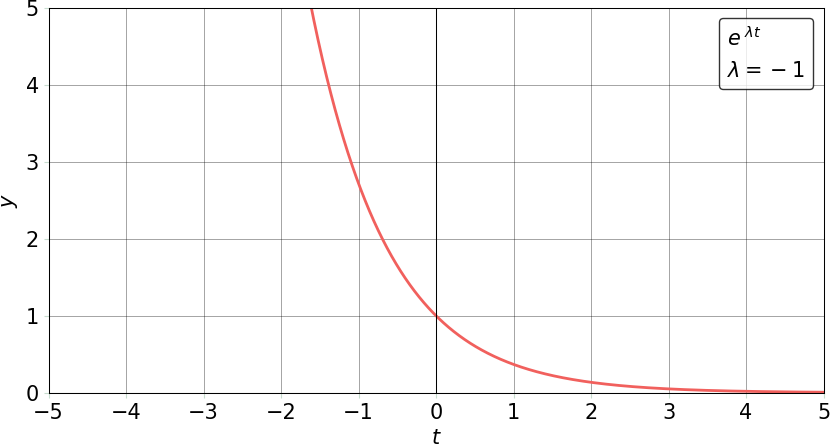
\includegraphics[width=0.4\textwidth]{Exponential Decay/Exact with -1.png}
\end{center}
\par \hspace*{1cm} If we restrict $\lambda$ to $\bR^{-}$, we have a simple\\
\hspace*{1cm} exponential curve that decays to zero as $t \rightarrow \infty$.\\
\columnbreak{}
\begin{center}
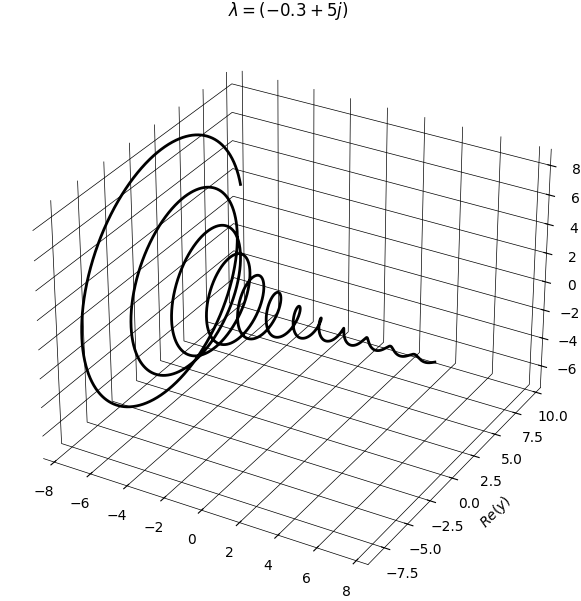
\includegraphics[width=0.4\textwidth]{Exponential Decay/Exact with (-0.3+5j).png}
\end{center}
\par \hspace*{1cm} If we allow $\lambda \in \bC$ and $Re(\lambda)<0$,\\
\hspace*{1cm} we get a spiral in the complex plane,\\
\hspace*{1cm} the radius of which decays to zero as $t \rightarrow \infty$.\\
\end{multicols}

\subsection{The Maclaurin Series}
The Taylor series is given by:
\[y(t) = \sum\limits_{n=0}^{\infty} \frac{{y}^{(n)}(a)}{n!}{(t-a)}^n\]
Setting $a=0$, we get the Maclaurin series for the exact solution:
\[y(t) = \sum\limits_{n=0}^{\infty} \frac{{(\lambda)}^n e^0}{n!}t^n = \sum\limits_{n=0}^{\infty} \frac{{(\lambda t)}^n}{n!} \quad\text{which we will denote}\; M(y)\]
This is a useful form for the exact solution -- we will see it pop up again later.

\subsection{Proponents of the Exponential Decay Problem}
\par There are a few pros to this choice of problem:
\begin{itemize}
    \item[$\cdot$] The exact solution is known and easily computed; it can be used to evaluate a numerical solution.
    \item[$\cdot$] The solution is a straightforward and well understood function.\\
    	  This simplicity allows us to focus on the numerical method.
    \item[$\cdot$] The problem is linear in $y(t)$, making the problem simple to work with.\\
    	  Again, our focus can stay on the numerical method.
    \item[$\cdot$] The graph of the exact solution is easy to visualise; the more chaotic outputs of the numerical methods can be compared to the smooth curve of the exact solution easily.
    \item[$\cdot$] Exponential decay is a model for many physical processes, including radioactive decay, population decline, and capacitor discharge.\\
    	  Quantities that decay relative to their current value appear frequently in nature.\\
    	  This means readers from many different disciplines may already possess an intuition for the problem.
    \item[$\cdot$] The problem is simple to generalise to complex numbers, allowing us to explore the stability of numerical methods in the complex plane.
    \item[$\cdot$] The Exponential Decay Problem is \term{stiff}; for certain method-step pairs, the numerical solution may oscillate wildly.\\
    	  This is exactly the kind of behaviour we want to avoid in a numerical method, when we are looking for stability.
\end{itemize}

\par Normally, when using the Exponential Decay Problem in a numerical analysis context, we would allow $\lambda \in \bC$ with $Re(\lambda)<0$.\\
However, for the purposes of this paper, we will restrict $\lambda$ to $\bR$ as we will be looking at $h \in \bC$ and we don't want to overcomplicate things.\\
Unless otherwise mentioned, we will assume that $\lambda \in \bR^{-}$ for the rest of this paper.\\

\par We will use the Exponential Decay Problem throughout this paper to derive a useful framework for the analysis of the stability of a numerical method.\\

\newpage
\section{Stability Analysis}

\subsection{Introduction}
\par In this section we will lay out a framework for analysing the stability of a numerical method.\\
To begin, we will introduce the concept of the stability function.\\
We will show how it can be used to define a stability region.\\
We will explore the stability region as the set of values for which a numerical method is stable.\\
Finally, we will extend this framework to view the stability of a numerical method in the context of complex time steps.\\

\subsection{Numerical Method: Forward Euler}

\par Let's consider a simple numerical method applied to the Exponential Decay Problem.\\
The Forward Euler method is a first-order numerical method for solving ODEs with a given initial condition.\\
Its algorithm can be defined as:
\[ y(t_{j+1}) = y(t_j) + h y'(t_j)\]
Where $h$ is the time step and $y_j$ is the numerical solution at time $t_j$, $j$ steps on from $t_0=0$.\\
This means $t_j = hj$.\\

\par For the Exponential Decay Problem, the Forward Euler method can be written as:
\[ y_{j+1} = y_j + h \lambda y_j \quad \text{where} \quad y_0 = 1\]
This gives us the following algorithm:
\[ y_{j+1} = (1 + h \lambda) y_j\]
This gives an approximation of the exact solution at time $t_j$ as follows:
\[ y_{j} = {(1 + h \lambda)}^j y_0 = {(1 + h \lambda)}^j = y(t_j) = y(hj) \approx e^{\lh j}\]

\par We can see that the Forward Euler method is stable if $|1 + h \lambda| < 1$;\\
both the exact solution and our approximation will decay to zero as $t \rightarrow \infty$.\\
The stability is dependent on the time step $h$ and the value of $\lambda$.\\
We can write this as $s(\lambda, h) = 1 + h \lambda$.\\
By analysing $s$ for different values of $\lambda$ and $h$,\\
we can infer the stability of the Forward Euler method for the Exponential Decay Problem.\\
We call $s$ the \term{stability function} of the Forward Euler method.

\subsection{The Stability Function and corresponding Stability Region}
\par By the same methodology, we can define the stability function for any numerical method by writing the algorithm in the form $y_{j+1} = s(\lambda, h) y_{j}$.\\
$s(\lambda, h)$ is the \term{stability function} of the numerical method with a time step $h$.\\
\textbf{Note:} This is equivalent to $y_{j} = {s(\lambda,h)}^{j} y_0$

\par The \term{stability region} of a numerical method is the set $S = \Big\{ (\lambda, h) \;\Big|\; |s(\lambda, h)| < 1\Big\} \subset \bC$\\
This follows from the definition of stability for our Exponential Decay Problem;\\
a method is stable if the numerical solution decays to zero as $t \rightarrow \infty$.\\
Clearly, $\Lim{j \rightarrow \infty}y_{j} = \Lim{j \rightarrow \infty}{s(\lambda,h)}^{j} y_0 = 0 \iff |s(\lambda, h)| < 1$.
Now, let's explore some examples of stability regions for different numerical methods.

\newpage
\subsubsection{Stability Region for Euler's Forward Method}
\begin{multicols}{2}
Euler's Forward Method has the stability function
\[s(\lambda, h) = 1 + \lh = \sum\limits_{n=0}^{1} \frac{{(\lh)}^n}{n!} = M(y) + \mathcal{O}((\lh)^2)\]
The corresponding stability region is 
\[S = \Big\{ (\lambda, h) \;\Big|\; |1 + \lh| < 1\Big\}\]
We can see this region plotted in red on the right; an open unit circle centred at $-1$.\\

For a given $\lambda \in \bC$, the method is stable for any step-size $h \in \bR$ such that $|1 + \lh| < 1$.\\

\par Expanding $\lambda = a + bi$, we get the restriction
\[|1 + (a + bi)h| < 1 \quad \implies \quad |(1+ah) + (bh)i| < 1\] 
\[\implies \quad a^2h^2 + 2ah + b^2h^2 < 0\]
\[a, b, h \in \bR \implies (a^2 +b^2)h^2 > 0\] 
\[\implies 2ah < 0 \text{ and } ||2ah|| > (a^2 + b^2)h^2\]
This aligns with our intuition for the problem;
\begin{itemize}
	\item[$\cdot$] For the exponential to decay,\\
	      we must have $Re(\lambda) = a < 0$.
	\item[$\cdot$] $h$ must be positive, as it is a time step.
\end{itemize}
\columnbreak{}
\vspace*{\fill}
\begin{center}
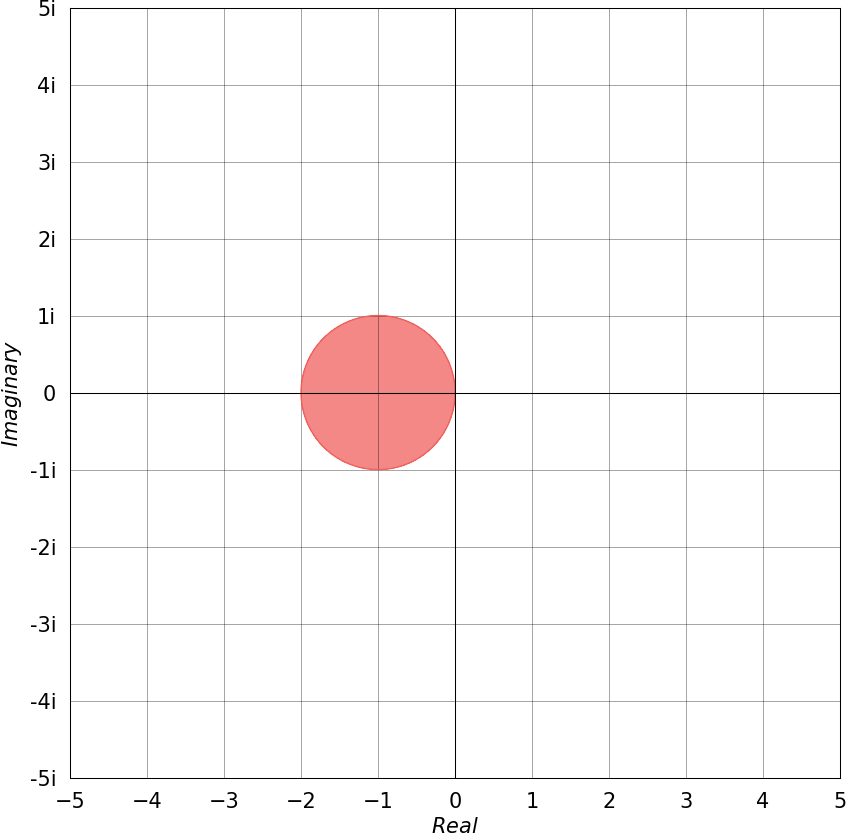
\includegraphics[width=0.49\textwidth]{Stability Regions/Graphs/Real 1-Step/Euler's Forward.png}
\end{center}
\vspace*{\fill}
\end{multicols}
Moreover, 
\[0 < (a^2 +b^2)h^2< ||2ah|| \quad\implies\quad 0 < h < \frac{||2a||}{a^2 + b^2} \quad\implies\quad 0 < h < \frac{2 ||Re(\lambda)||}{{|\lambda|}^2}\]
This is also intuitive; if we imagine $\lambda$ growing linearly, $h$ must shrink quadratically so that their product $\lh$ stays inside the stability region.\\
%\textbf{Note to self: This feels similar to the inversion of a point through a circle in $\bC$.}

\subsubsection{Stability Region for Euler's Backward Method}
\begin{multicols}{2}
\vspace*{\fill}
\begin{center}
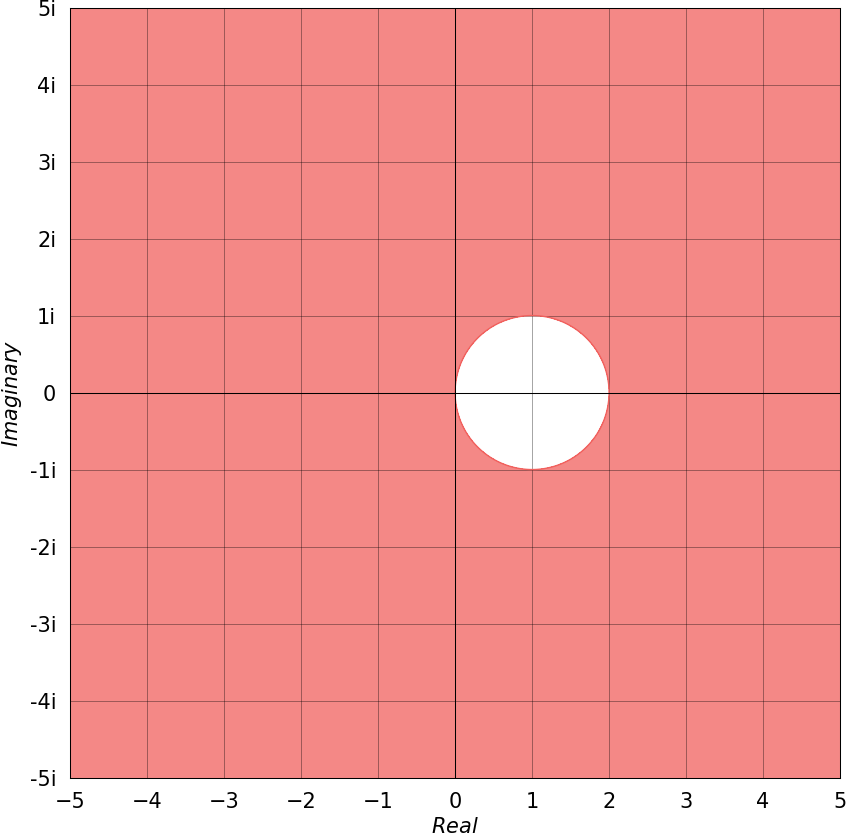
\includegraphics[width=0.49\textwidth]{Stability Regions/Graphs/Real 1-Step/Euler's Backward.png}
\end{center}
\vspace*{\fill}
\columnbreak{}
Euler's Backward Method can be written as
\[y_{j+1} = y_j + h.y'(t_{j+1})\]
\[\implies y_{j+1} = y_j + h(\lambda y_{j+1}) \implies y_{j+1} = \frac{1}{1 - \lh}y_j\]
Thus, the stability function is
\[s(\lambda, h) = \frac{1}{1 - \lh}\]
The corresponding stability region is
\[S = \Big\{ (\lambda, h) \;\Big|\; \left|\frac{1}{1 - \lh}\right| < 1\Big\}\]
This is plotted in red on the left; the region outside a unit circle centred at $1$.\\
The white region of instability is exactly the stability region for Euler's Forward Method, flipped about Imaginary axis.\\

\par We could run through the same algebraic proceedure as before, expanding $\lambda$ and rearranging, and we would find that 
\[h > \frac{2 Re(\lambda)}{{|\lambda|}^2}\]
\end{multicols}
This is a more lax restriction than the $0<h$ that we have already established.\\
In fact, this tells us that any positive $h$ will give a stable solution, regardless of the value of $\lambda$.\\
This is a property called \term{Absolute Stability} or \term{A-Stability}.\\
This is often characterised by a stability region that covers the entire left half-plane, as we see here.\\

\subsubsection{Stability Region for Runge-Kutta 4}
\begin{multicols}{2}
\vspace*{\fill}

Runge-Kutta 4 can be written as
\[y_{j+1} = y_j + \frac{h}{6}(k_1 + 2k_2 + 2k_3 + k_4)\]
Where $\phi(t,y) = y'(t) = \lambda y$
\begin{flalign*}
	k_1 &= \phi(t_j, y_j) \quad &k_2 = \phi(t_j + \frac{h}{2}, y_j + \frac{h}{2}k_1) && \\
	k_3 &= \phi(t_j + \frac{h}{2}, y_j + \frac{h}{2}k_2) \quad &k_4 = \phi(t_j + h, y_j + hk_3) &&
\end{flalign*}
For the Exponential Decay Problem, we get
\[y_{j+1} = (1 + \lh + \frac{{(\lh)}^2}{2} + \frac{{(\lh)}^3}{6} + \frac{{(\lh)}^4}{24})y_j\]
The stability function is
\[s(\lambda, h) = \sum\limits_{n=0}^{4}\frac{{(\lh)}^n}{n!} = M(y) + \mathcal{O}((\lh)^5)\]
The corresponding stability region is
\[S = \Big\{ (\lambda, h) \;\Big|\; \left|\sum\limits_{n=0}^{4}\frac{{(\lh)}^n}{n!}\right| < 1\Big\}\]

\vspace*{\fill}
\columnbreak{}
\begin{center}
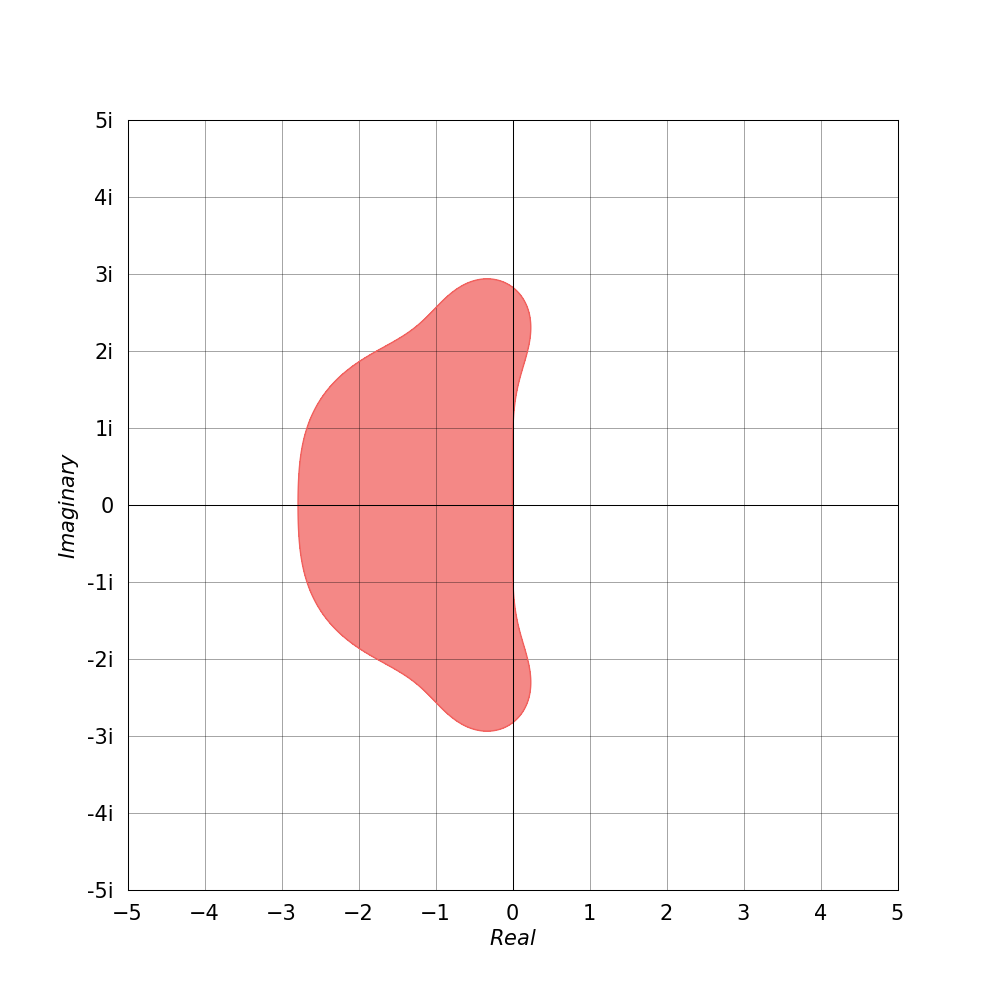
\includegraphics[width=0.49\textwidth]{Stability Regions/Graphs/Real 1-Step/Runge-Kutta 4.png}
\end{center}
\end{multicols}

\subsection{Interpretation of Stability Regions}

\par The stability region $S = \Big\{ (\lambda, h) \;\Big|\; |s(\lambda, h)| < 1\Big\} \in \bC$ is a set of values for which a numerical method is stable for the Exponential Decay Problem.\\
We always restrict $h \in {\bR}^{+}$, as it is a time step.\\
We have two separate cases for $\lambda$:
\begin{itemize}
	\item[$\cdot$] $\lambda \in {\bR}^{-}$:\;\; $S$ corresponds to $\big\{{s(\lambda, h)}^2 < 1\big\}$. \;\; Of course, $\lambda, h \in \bR \implies S \subset \bR$.
	\item[$\cdot$] $\lambda \in \bC\setminus\bR$ with $Re(\lambda) < 1$:\;\; $S$ corresponds to $\Big\{\big(s(\lambda, h)\big)\big(\,\overline{s(\lambda, h)}\,\big) < 1\Big\}$.
\end{itemize}

\par From here, one can derive bounds on $h$ for a given value of $\lambda$, or vice versa.\\
We did this with Euler's Forward and Backward methods above.\\
The Runge-Kutta 4 method is more complicated, as the two cases of $\lambda$ each give a polynomial of degree 8.\\

\par Below we have graphs for the cases where $\lambda$ is real or complex,\\
the same as we introduced for the Exponential Decay Problem.\\
In black is the exact solution. In colour are the numerical solutions due to the method in question.\\
These $(\lambda, h)$ pairs were found by first picking a value of $\lambda$ and then finding $h$ values which met the stability condition.\\
In green $(\lambda, h) \in S$.\\
In red $(\lambda, h) \notin S$.
\newpage
\subsubsection{Euler's Forward Method}
\begin{multicols}{2}
	\begin{center}
	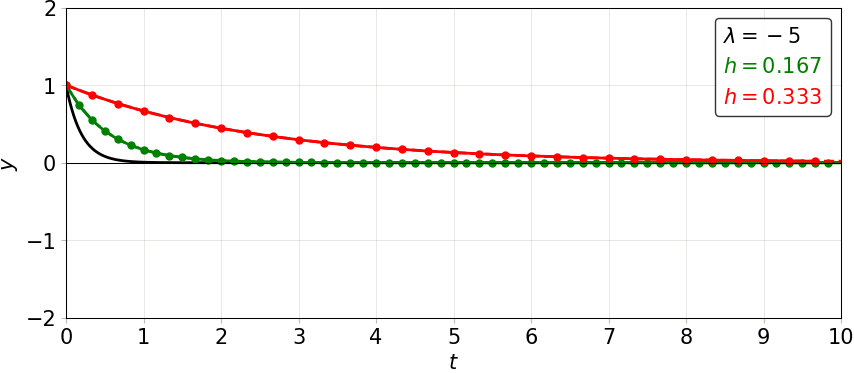
\includegraphics[width=0.49\textwidth]{Exponential Decay/Exact vs Method/Euler's Forward real.png}
        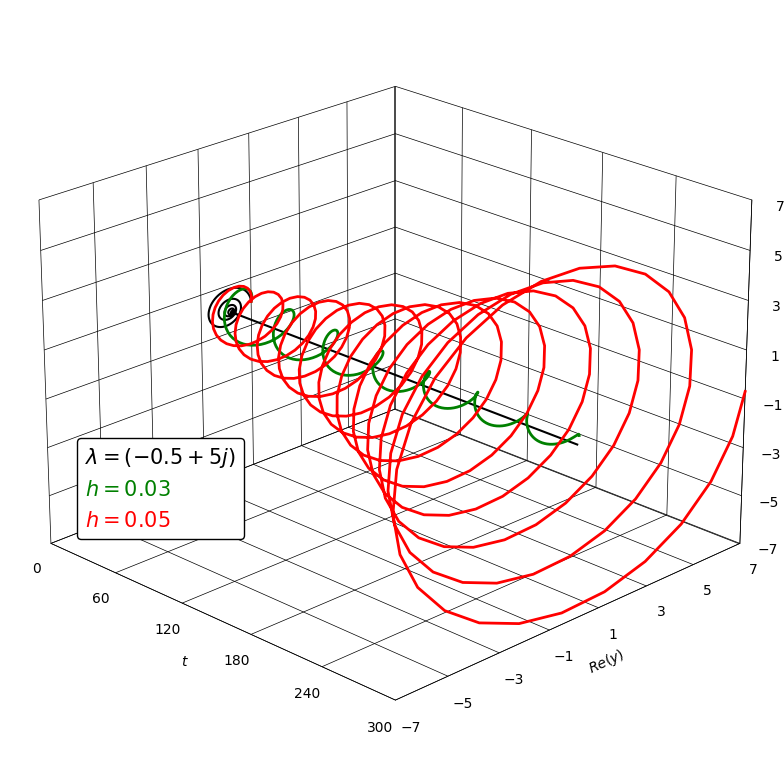
\includegraphics[width=0.49\textwidth]{Exponential Decay/Exact vs Method/Euler's Forward complex.png}
	\end{center}
\columnbreak{}
	\par On the left are the aforementioned graphs for Euler's Forward Method.\\
	
	\par First is the case where $\lambda \in \bR^{-}$.\\
	The exact solution decays quickly in black, very close to $t=0$.
	The numerical solution converges to the exact solution for $h = 1/6$ in green.\\
	For $h = 5/12$, the numerical solution oscillates and diverges in red.\\
	The oscillation is due to the stability function\\
	$s(\lambda, h) = 1 + \lh = 1 + -5\cdot\frac{5}{12} = \frac{-13}{12}$\\
	The $j^{th}$ term of the numerical solution is ${s(\lambda, h)}^j = {\left(\frac{-13}{12}\right)}^j$.\\
	Of course, natural powers of negative numbers oscilate between positive and negative values.\\
	$|\frac{-13}{12}| > 1 \implies$ the numerical solution diverges.\\

	\par Second is the case where $\lambda \in \bC$.\\
	The exact solution decays quickly in black, very close to the $t=0$ plane.\\
	The green, valid $h$ value converges as $t$ increases, but the red, invalid $h$ value diverges.\\
        
        \par While this 3D graph might not be the clearest, it took quite a lot of messing with values of $h$ and $\lambda$ to find one so demonstrative.\\
	The reader is encouraged to play with values for $h$ and $\lambda$ in \\
	`/Python/Exponential Decay/Exact vs Method.py'\\
	of the GitHub repository~\cite{GitHub_Repo} to see for themselves.\\
	This has the added benefit of allowing you to rotate the graph to see the behaviour from different angles.
\end{multicols}

\subsubsection{Euler's Backward Method}
\begin{multicols}{2}
	As mentioned before, Euler's Backward Method is A-Stable.\\
	This means that for any $\lambda \in \bC$ with $Re(\lambda) < 1$, the method is stable for any $h \in \bR^{+}$.\\
	As a result, there is no choice of $(\lambda, h)$ that will give us a divergent graph.\\
	For $\lh$ to land in the white disk of instability, either $h$ must be negative or $Re(\lambda) > 1$.\\
	Both of these are nonsensical for our Exponential Decay Problem.\\
	Instead, these graphs show two different stable $h$ values for the same $\lambda$ value.\\
	For $\lambda \in \bR^{-}$ below, the numerical solution converges to the exact solution for both step sizes.\\
	\begin{center}
	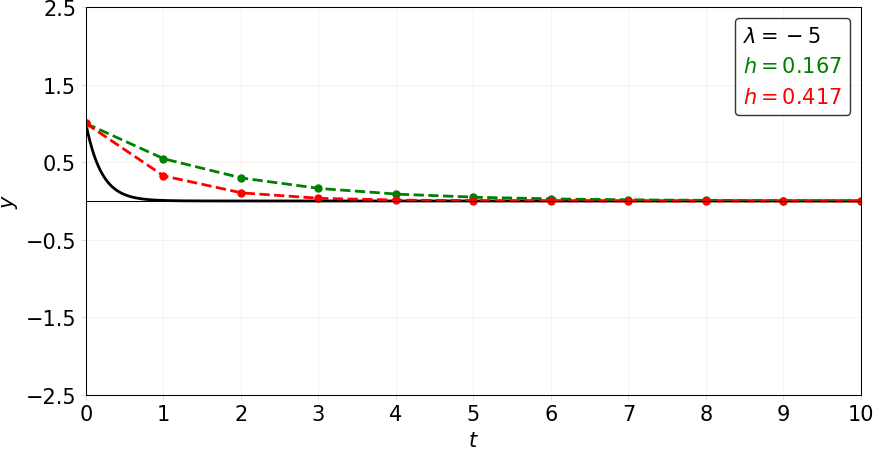
\includegraphics[width=0.49\textwidth]{Exponential Decay/Exact vs Method/Euler's Backward real.png}
	\end{center}
	\columnbreak{}
	\vspace*{-1.5cm}
	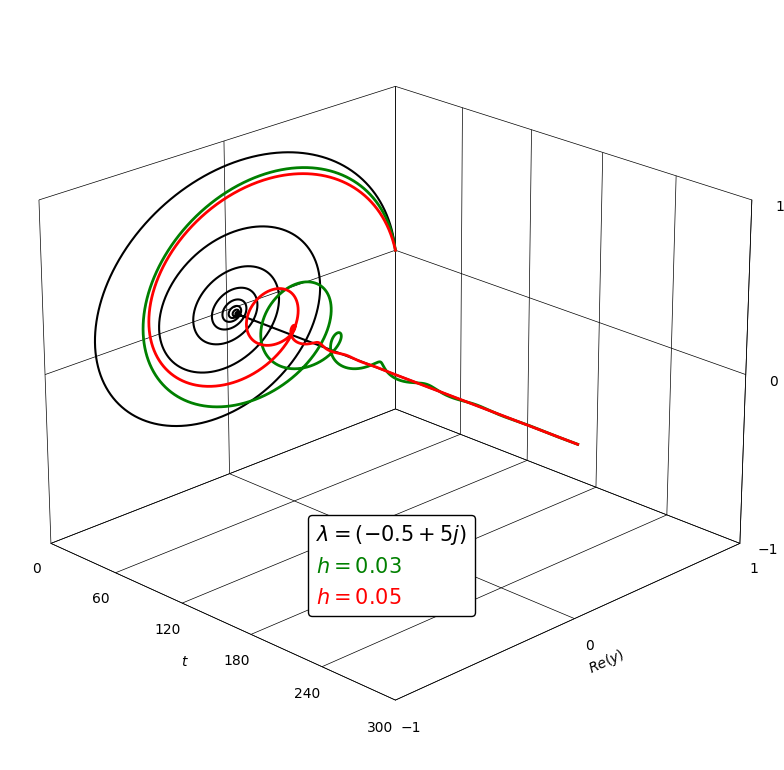
\includegraphics[width=0.49\textwidth]{Exponential Decay/Exact vs Method/Euler's Backward complex.png}
	For $\lambda \in \bC$ above, the method converges to the exact solution for both step sizes.\\
	There is no divergence, as we have already established.\\
	Interestingly, the method converges faster for the larger step size.\\
	The subsequent section on Stability Magnitudes will explain this behaviour.
\end{multicols}
\newpage
\subsubsection{Runge-Kutta 4}
\begin{multicols}{2}
	The same properties hold true for Runge-Kutta 4, as we demonstrated for Euler's Forward, though we choose different values of $h$ and $\lambda$ for aesthetic clarity.\\
	\vspace*{2cm}
	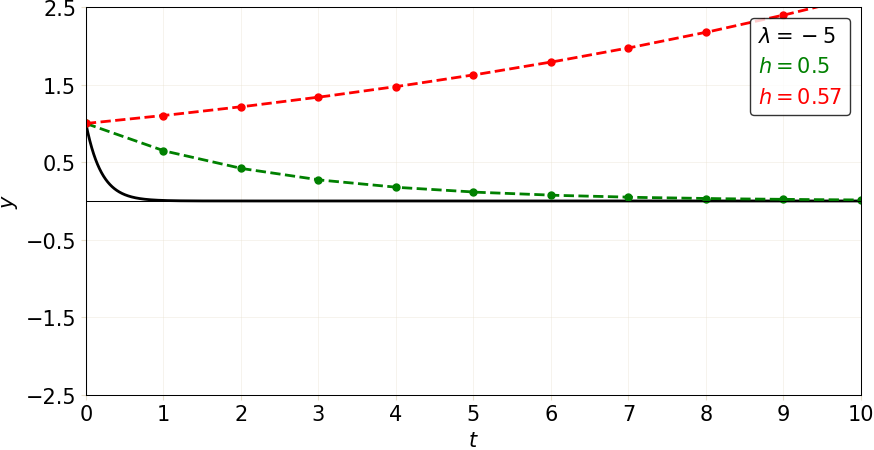
\includegraphics[width=0.49\textwidth]{Exponential Decay/Exact vs Method/Runge-Kutta 4 real.png}
\columnbreak{}
\begin{center}
	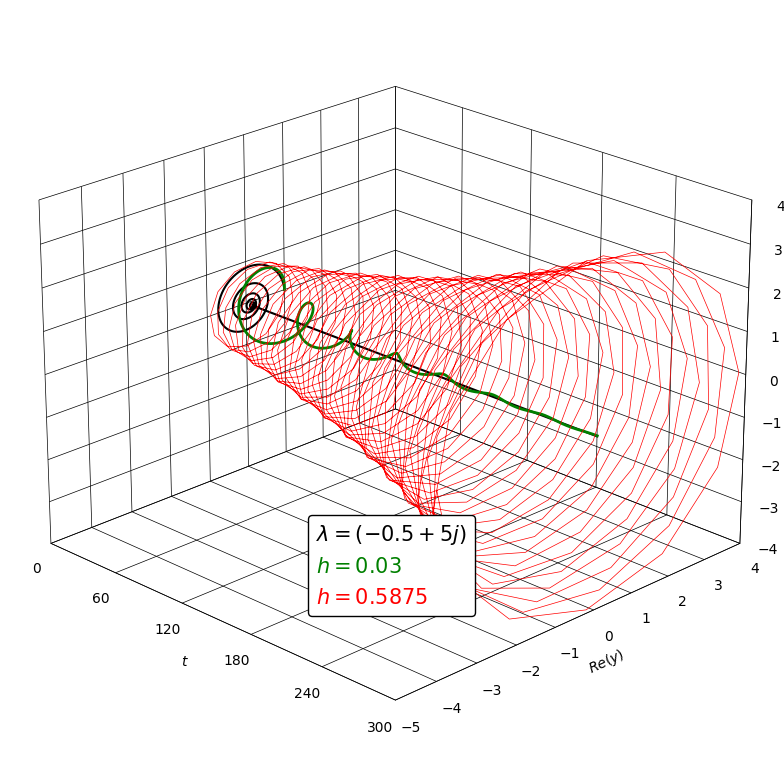
\includegraphics[width=0.49\textwidth]{Exponential Decay/Exact vs Method/Runge-Kutta 4 complex.png}
\end{center}
\end{multicols}
\newpage
\subsection{Stability Magnitudes}
So far we have been looking at stability regions given by $|s(\lambda, h)| < 1$.\\
While this bound is a sufficient condition for stability, we are not truly utilising the metric.\\
In this section, we'll explore $|s(\lambda, h)|$ in a little more detail.\\
The plots below show the magnitude of the stability function for different values of $\lh$.\\
We have limited these to display only the magnitudes within the region $S$ for clarity; $|s(\lambda, h)| < 1$.\\
The 3D plots show the magnitudes $|s(\lambda, h)|$ above the base plane $S$.\\
The magnitudes have been projected down onto the base plane as colour plots.\\
We show these colour plots separately in the second graphs.\\
While on the first graphs, these colour gradients are continuous, on the second graphs we have discretised them.\\
This is so that for the third graphs we can create a correspondance with the plotted numerical solutions.\\
We'll only present the Exponential Decay graphs for real $\lambda$ here, as the complex $\lambda$ graphs are, well, complex. No need to spiral out of control.\\
Their behavior is the same as for the real $\lambda$ graphs, with tighter, faster decaying spirals as $\lh$ lands in brighter areas of the colour plot.\\
\subsubsection{Euler's Forward Method}
\begin{multicols}{2}
	\begin{center}
	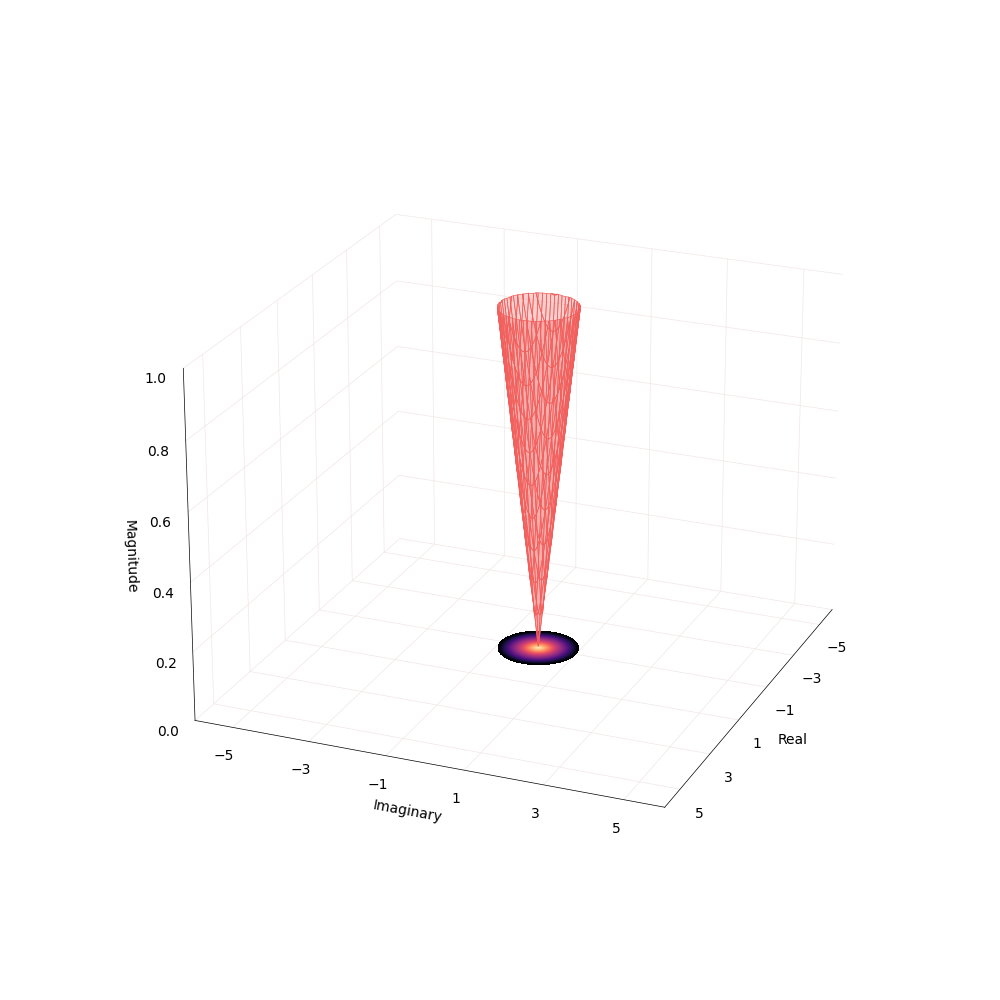
\includegraphics[width=0.49\textwidth]{Stability Magnitude/3D/Euler's Forward.png}
	\end{center}
	\columnbreak{}
	\begin{center}
	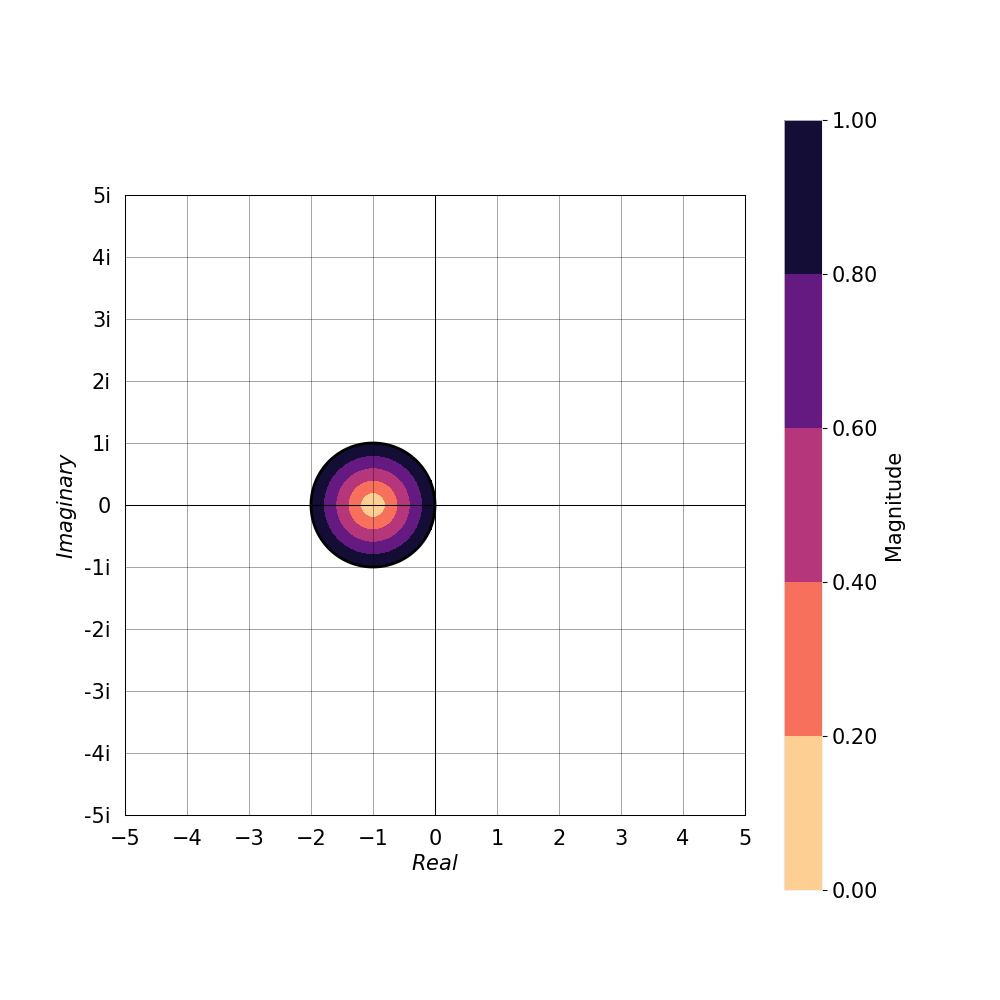
\includegraphics[width=0.45\textwidth]{Stability Magnitude/Color/Euler's Forward.png}
	\end{center}
\end{multicols}
\begin{multicols}{2}
	\begin{center}
		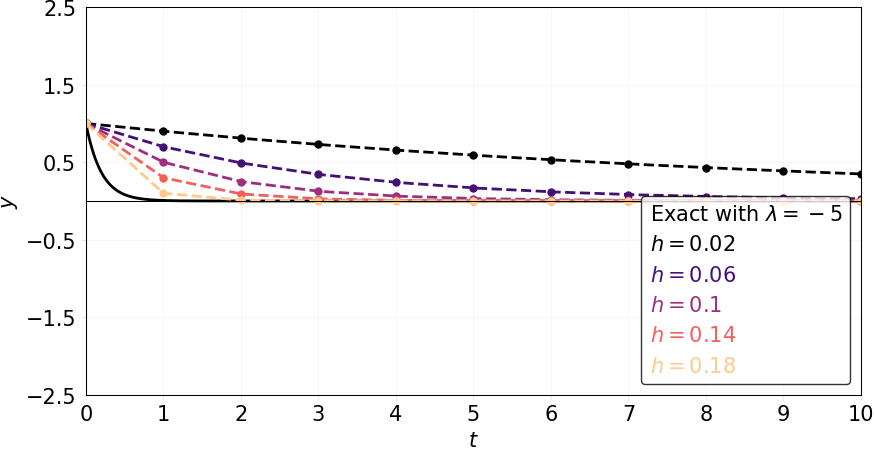
\includegraphics[width=0.49\textwidth]{Stability Magnitude/Exponential Decay/Euler's Forward.png}
	\end{center}
	\columnbreak{}
	We can see smaller magnitudes correspond to a tighter fit to the exact solution.\\
	This aligns with our intuition; for a derivative,\\
	we allow $h \rightarrow 0$ to obtain the exact solution.\\
	Recall, in a computational context, we're looking for the largest $h$ that will give us a stable solution, that has an error within our tolerance.\\
	Between each point on the graph, $\frac{1}{h}$ calculations are done to find the next point.\\
	For larger $h$, the method is less accurate, but faster.\\
\end{multicols}

\newpage
\subsubsection{Euler's Backward Method}
\begin{multicols}{2}
	\begin{center}
	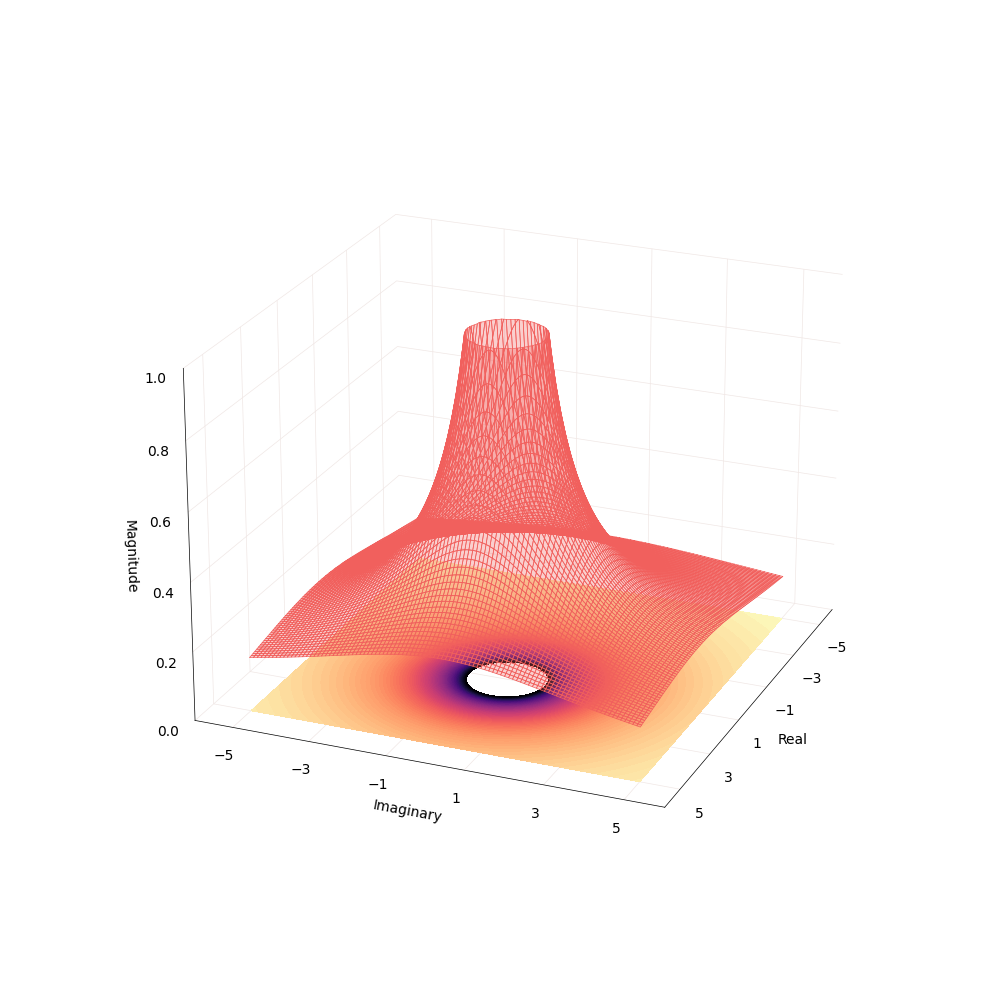
\includegraphics[width=0.49\textwidth]{Stability Magnitude/3D/Euler's Backward.png}
	\end{center}
	\columnbreak{}
	\begin{center}
	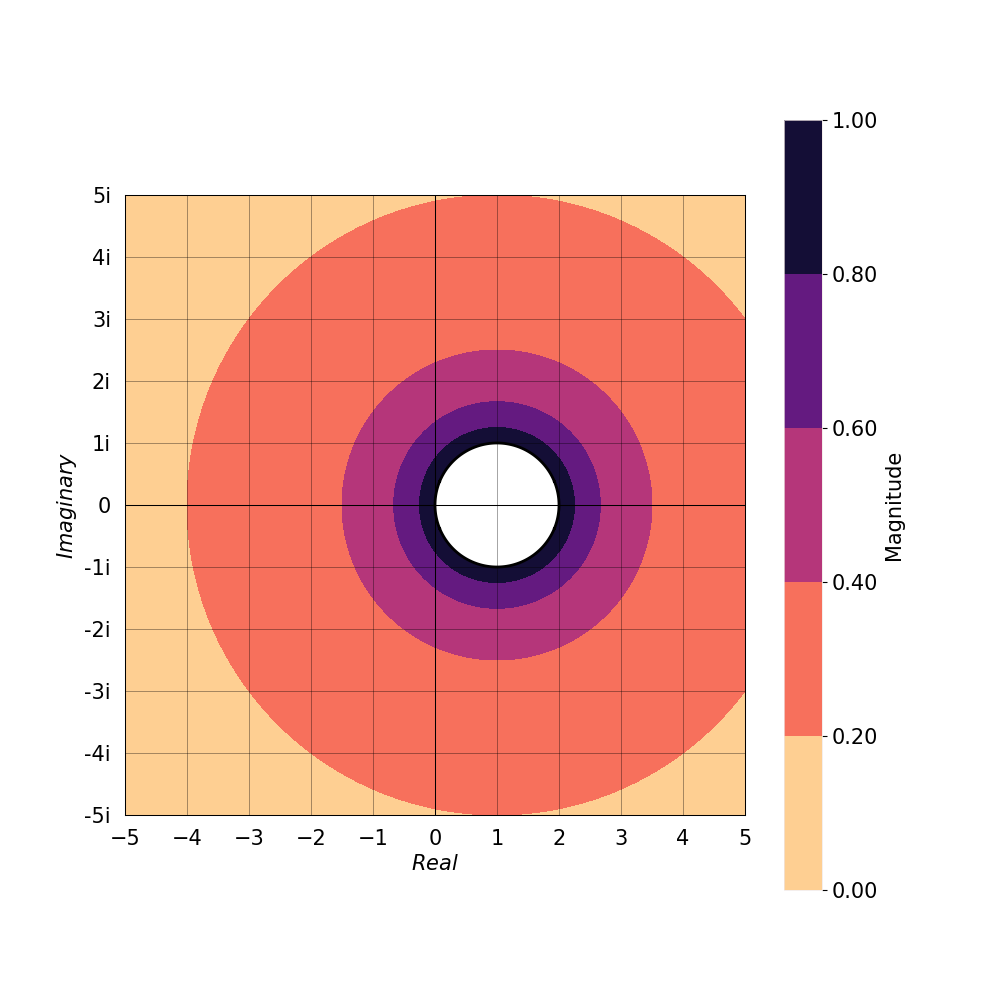
\includegraphics[width=0.45\textwidth]{Stability Magnitude/Color/Euler's Backward.png}
	\end{center}
\end{multicols}
\begin{multicols}{2}
	\begin{center}
		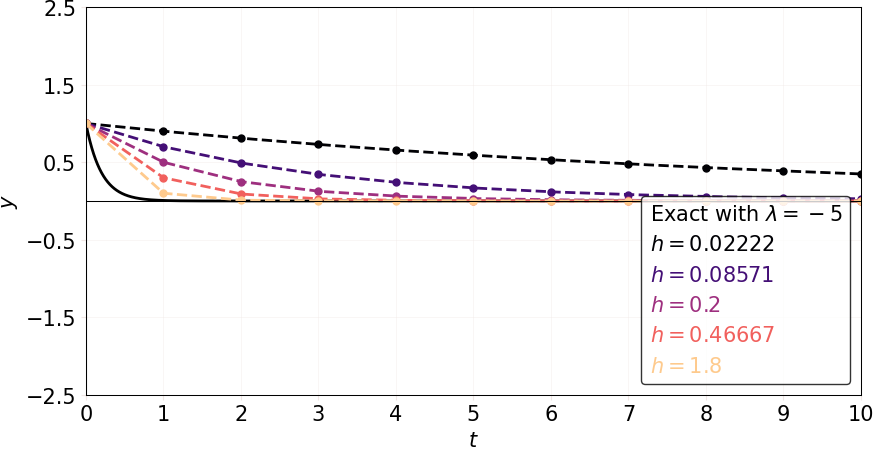
\includegraphics[width=0.49\textwidth]{Stability Magnitude/Exponential Decay/Euler's Backward.png}
	\end{center}
	\columnbreak{}
	As we have already established, Euler's Backward Method is A-Stable.\\
	Any choice of $h \in \bR^{+}$ will give a stable solution for any $\lambda \in \bC$ with $Re(\lambda) < 1$.\\
	It is impossible to pick such $(\lambda, h)$ values that will give $\lambda h$ in the white circle.\\
	By nature of the stability function $s(\lambda, h) = \frac{1}{1 - \lh}$, larger values of $h$ will give a smaller magnitudes; a tighter fit to the exact solution.\\
	This indicates why implicit methods like Euler's Backward are often used for stiff problems; they can be more accurate for larger time steps.\\
\end{multicols}

\subsubsection{Runge-Kutta 4}
\begin{multicols}{2}
	\begin{center}
	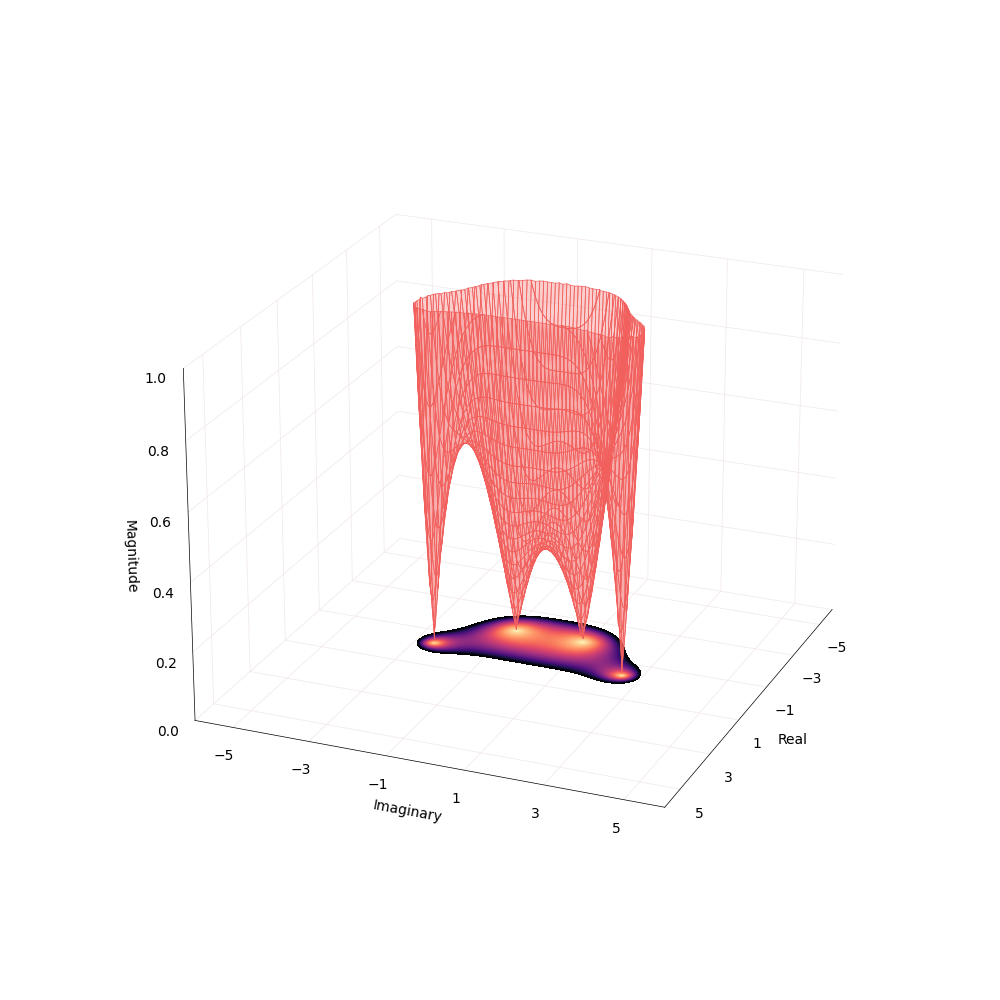
\includegraphics[width=0.49\textwidth]{Stability Magnitude/3D/Runge-Kutta 4.png}
	\end{center}
	\columnbreak{}
	\begin{center}
	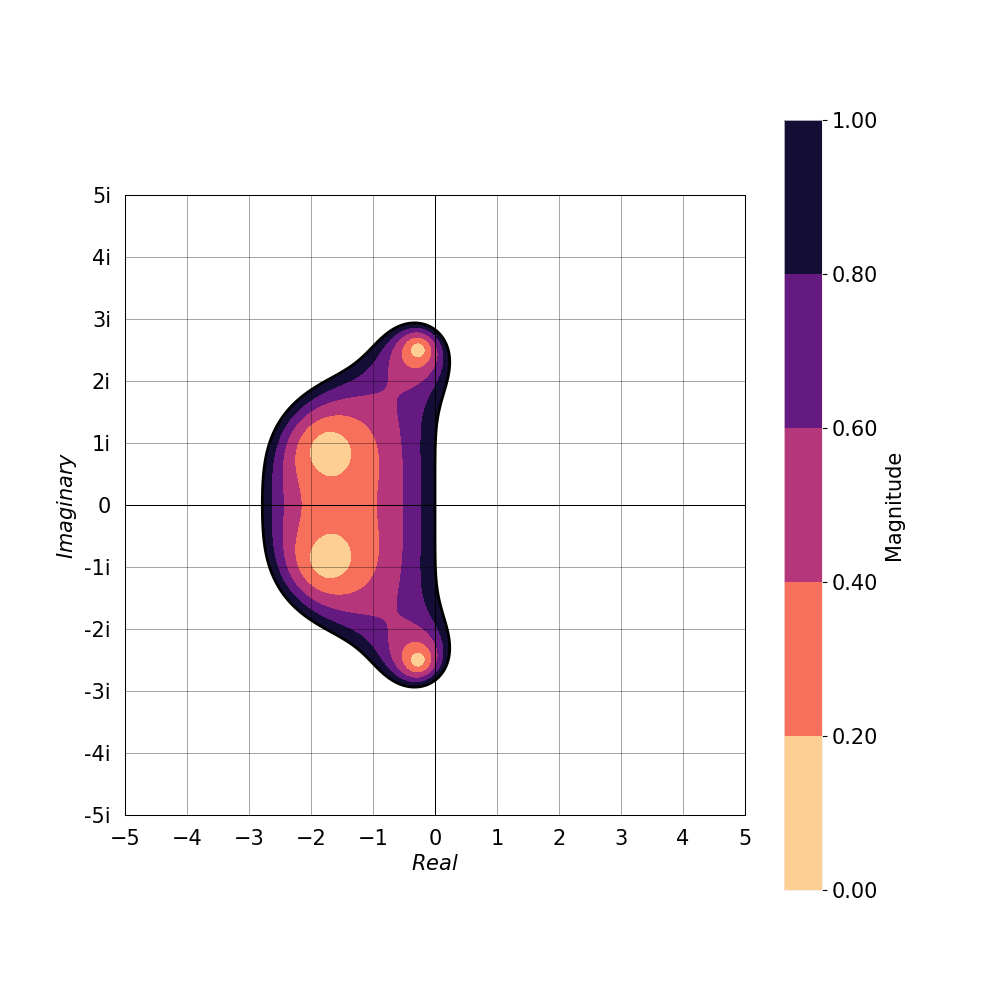
\includegraphics[width=0.45\textwidth]{Stability Magnitude/Color/Runge-Kutta 4.png}
	\end{center}
\end{multicols}
\begin{multicols}{2}
	\begin{center}
		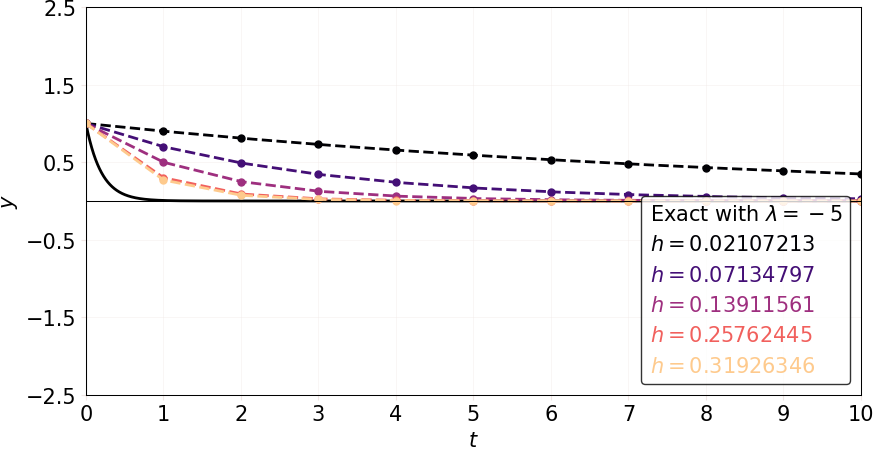
\includegraphics[width=0.49\textwidth]{Stability Magnitude/Exponential Decay/Runge-Kutta 4.png}
	\end{center}
	\columnbreak{}
	The same general observations as Euler's Forward Method hold true for Runge-Kutta 4.\\
	The values of $h$ here were calculated numerically, rather than algebraically.\\
	Check out `/Python/Stability Magnitude/Rk4 = c.py' in the GitHub repository~\cite{GitHub_Repo} for the code.\\
\end{multicols}

\newpage
\section{Complex Time-Steps}
So far, we have restricted our time-steps to the real domain.\\
It has often proven useful to extend the analysis of a problem to the complex domain.\\
Motivated by a paper by \textit{George, Yung and Mangan}\cite{walking_into_the_complex_domain}, we will have a look at the stability of numerical methods when the chosen time-step is complex.\\
They state: \begin{quote} \textit {Most numerical methods for time integration use real time steps. Complex time steps provide an additional degree of freedom, as we can select the magnitude of the step in both the real and imaginary directions. By time stepping along specific paths in the complex plane, integrators can gain higher orders of accuracy or achieve expanded stability regions.}\end{quote}

\subsection{Complex 2-Step}
\begin{multicols}{2}
\par We want to take an overall step of size $h \in \bR$ comprised of two steps $z_1, z_2 \in \bC$ such that $z_1 + z_2 = h$.\\
We can set $z_1 = a + bi$ and $z_2 = h - a - bi$.\\

\par For analysing our numerical methods, we require a comparable implementation of the real step setup.\\
A real 2-step method where we take a step of size $\frac{h}{2}$ allows us to take two steps and go the same distance as the complex 2-step method.\\
We can write this real 2-step method as
\[y_{j+1} = s(\lambda, \frac{h}{2}) y_{j+\frac{1}{2}} = s(\lambda, \frac{h}{2}) s(\lambda, \frac{h}{2}) y_j = {s(\lambda, \frac{h}{2})}^{2} y_j\]

\par We can write the complex 2-step method as 
\[y_{j+1} = s(\lambda, z_1) y_{j+\frac{1}{2}} = s(\lambda, z_1) s(\lambda, z_2) y_j\]
\vspace*{\fill}
\columnbreak{}
% Triangle diagram
\begin{tikzpicture}
	\draw[->] (0,0) -- (8,0) node[right] {$Re$};
	\draw[->] (0,0) -- (0,8) node[above] {$Im$};
	\draw[-, color=orange] (0,0) -- (5,7) node[midway, shift={(-0.2,0)}, left] {$z_1$};
	\draw[-, color=orange] (5,7) -- (7,0) node[midway, shift={(0.1,0)}, right] {$z_1 + z_2$};
	\draw[color=purple] (0,0) -- (7,0) node[midway, below] {$h$};
\end{tikzpicture}
\end{multicols}


\subsection{Complex Conjugate Pairs}
\begin{multicols}{2}
% Triangle diagram
\begin{tikzpicture}
	\draw[->] (0,0) -- (7,0) node[right] {$Re$};
	\draw[->] (0,0) -- (0,4.5) node[above] {$Im$};
	\draw[-, color=orange] (0,0) -- (3,3.5) node[midway, shift={(-0.2,0)}, left] {$z$};
	\draw[-, color=orange] (3,3.5) -- (6,0) node[midway, shift={(0.1,0)}, right] {$z + \bar{z}$};
	\draw[-, color=purple] (0,0) -- (3,0) node[midway, below] {$\frac{h}{2}$};
	\draw[-, color=purple] (3,0) -- (6,0) node[midway, below] {$\frac{h}{2}$};
	\draw[-, color=blue] (3,0) -- (3,3.5) node[midway, right] {$b$};
\end{tikzpicture}
\columnbreak{}
\par When we restrict the exponential decay problem by $\lambda \in \bR$, we also find that $s(\lambda, z_1) s(\lambda, z_2) \in \bR$\\
This is because any value attained by $e^{\lambda t}$ is real.\\
This restricts the values of $z_1$ and $z_2$, as any imaginary terms in $s(\lambda, z_1) s(\lambda, z_2)$ must cancel out.\\

\par One particularly simple family of such complex pairs is defined by setting $a = \frac{h}{2}$\\
This necessitates $z_2 = \bar{z_1}$\\
We will refer to this family as the \term{complex conjugate step pairs}.\\
\end{multicols}

\subsection{Stability of 2-Step Methods for Complex Conjugate Step Pairs}
\par In this section we will compare the stability regions for the real and complex 2-step methods.\\
The real step size is given by $\frac{h}{2}$\\
The complex conjugate step pair is given by $z = \frac{h}{2} + bi$ and $\bar{z} = \frac{h}{2} - bi$\\
The plots in this section show the regions of stability $S = \{\lh : |s(\lambda, h)| \leq 1\}$ for the case where $b=a=\frac{\lh}{2}$\\
We will have a look at varying $b$ in a subsequent section.\\

\newpage
\subsubsection{Euler's Forward 2-Step}
\begin{theorem}\textbf{Euler's Forward Complex Step Pairs must be Conjugate for $\lambda \in \bR$}\\
\par For the exponential decay problem, $y=e^{\lambda t}$, let $\lambda \in \bR$\\
Let $z_1 = a_1 + b_1i$ and $z_2 = a_2 + b_2i$ be a complex step pair for Euler's Forward 2-Step Method.\\
Then we must have $z_2 = \bar{z_1}$\\
\par\textbf{Proof:}
\[\lambda \in \bR \implies y_{j}, y_{j+1} \in \bR\]
Euler's Forward 2-Step Method is given by:
\begin{flalign*}
	y_{j+1} &= s(\lambda, z_1) s(\lambda, z_2)\; y_j && \\
	&= \Big(1 + z_1\Big)\Big(1 + z_2\Big)\; y_j && \\
	&= \Big(1+a_1+b_1 i\Big)\Big(1+a_2+b_2 i\Big)\; y_j && \\
	&= \Bigg(\Big(1 + a_1 + a_2 +a_1 a_2 - b_1 b_2\Big) + \Big(b_1 + b_2 + a_1 b_2 + a_2 b_1\Big)i\Bigg)\; y_j &&
\end{flalign*}
\[y_{j+1} \in \bR \implies Im(y_{j+1}) = 0 \implies b_1 + b_2 + a_1 b_2 + a_2 b_1 = 0 \implies (1+a_1)b_2 + (1+a_2)b_1 = 0\]
\[z_1+z_2 = h \in \bR \implies a_1+a_2 + (b_1+b_2)i = h \implies b_1+b_2 = 0 \implies b_1 = -b_2\]
\[(1+a_1)b_2 + (1+a_2)b_1 = 0 \implies (1+a_1)b_2 - (1+a_2)b_2 = 0 \implies b_2 = 0 = b_1 \text{ or } a_1 = a_2\]
Thus, $z_1, z_2 \in \bC \implies a_1 = a_2$ and $b_1 = -b_2$
\[\therefore z_1 = a_1 + b_1i \text{ and } z_2 = a_1 - b_1i \implies z_2 = \bar{z_1} \qquad\square\]
\end{theorem}
\begin{multicols}{2}
\begin{center}
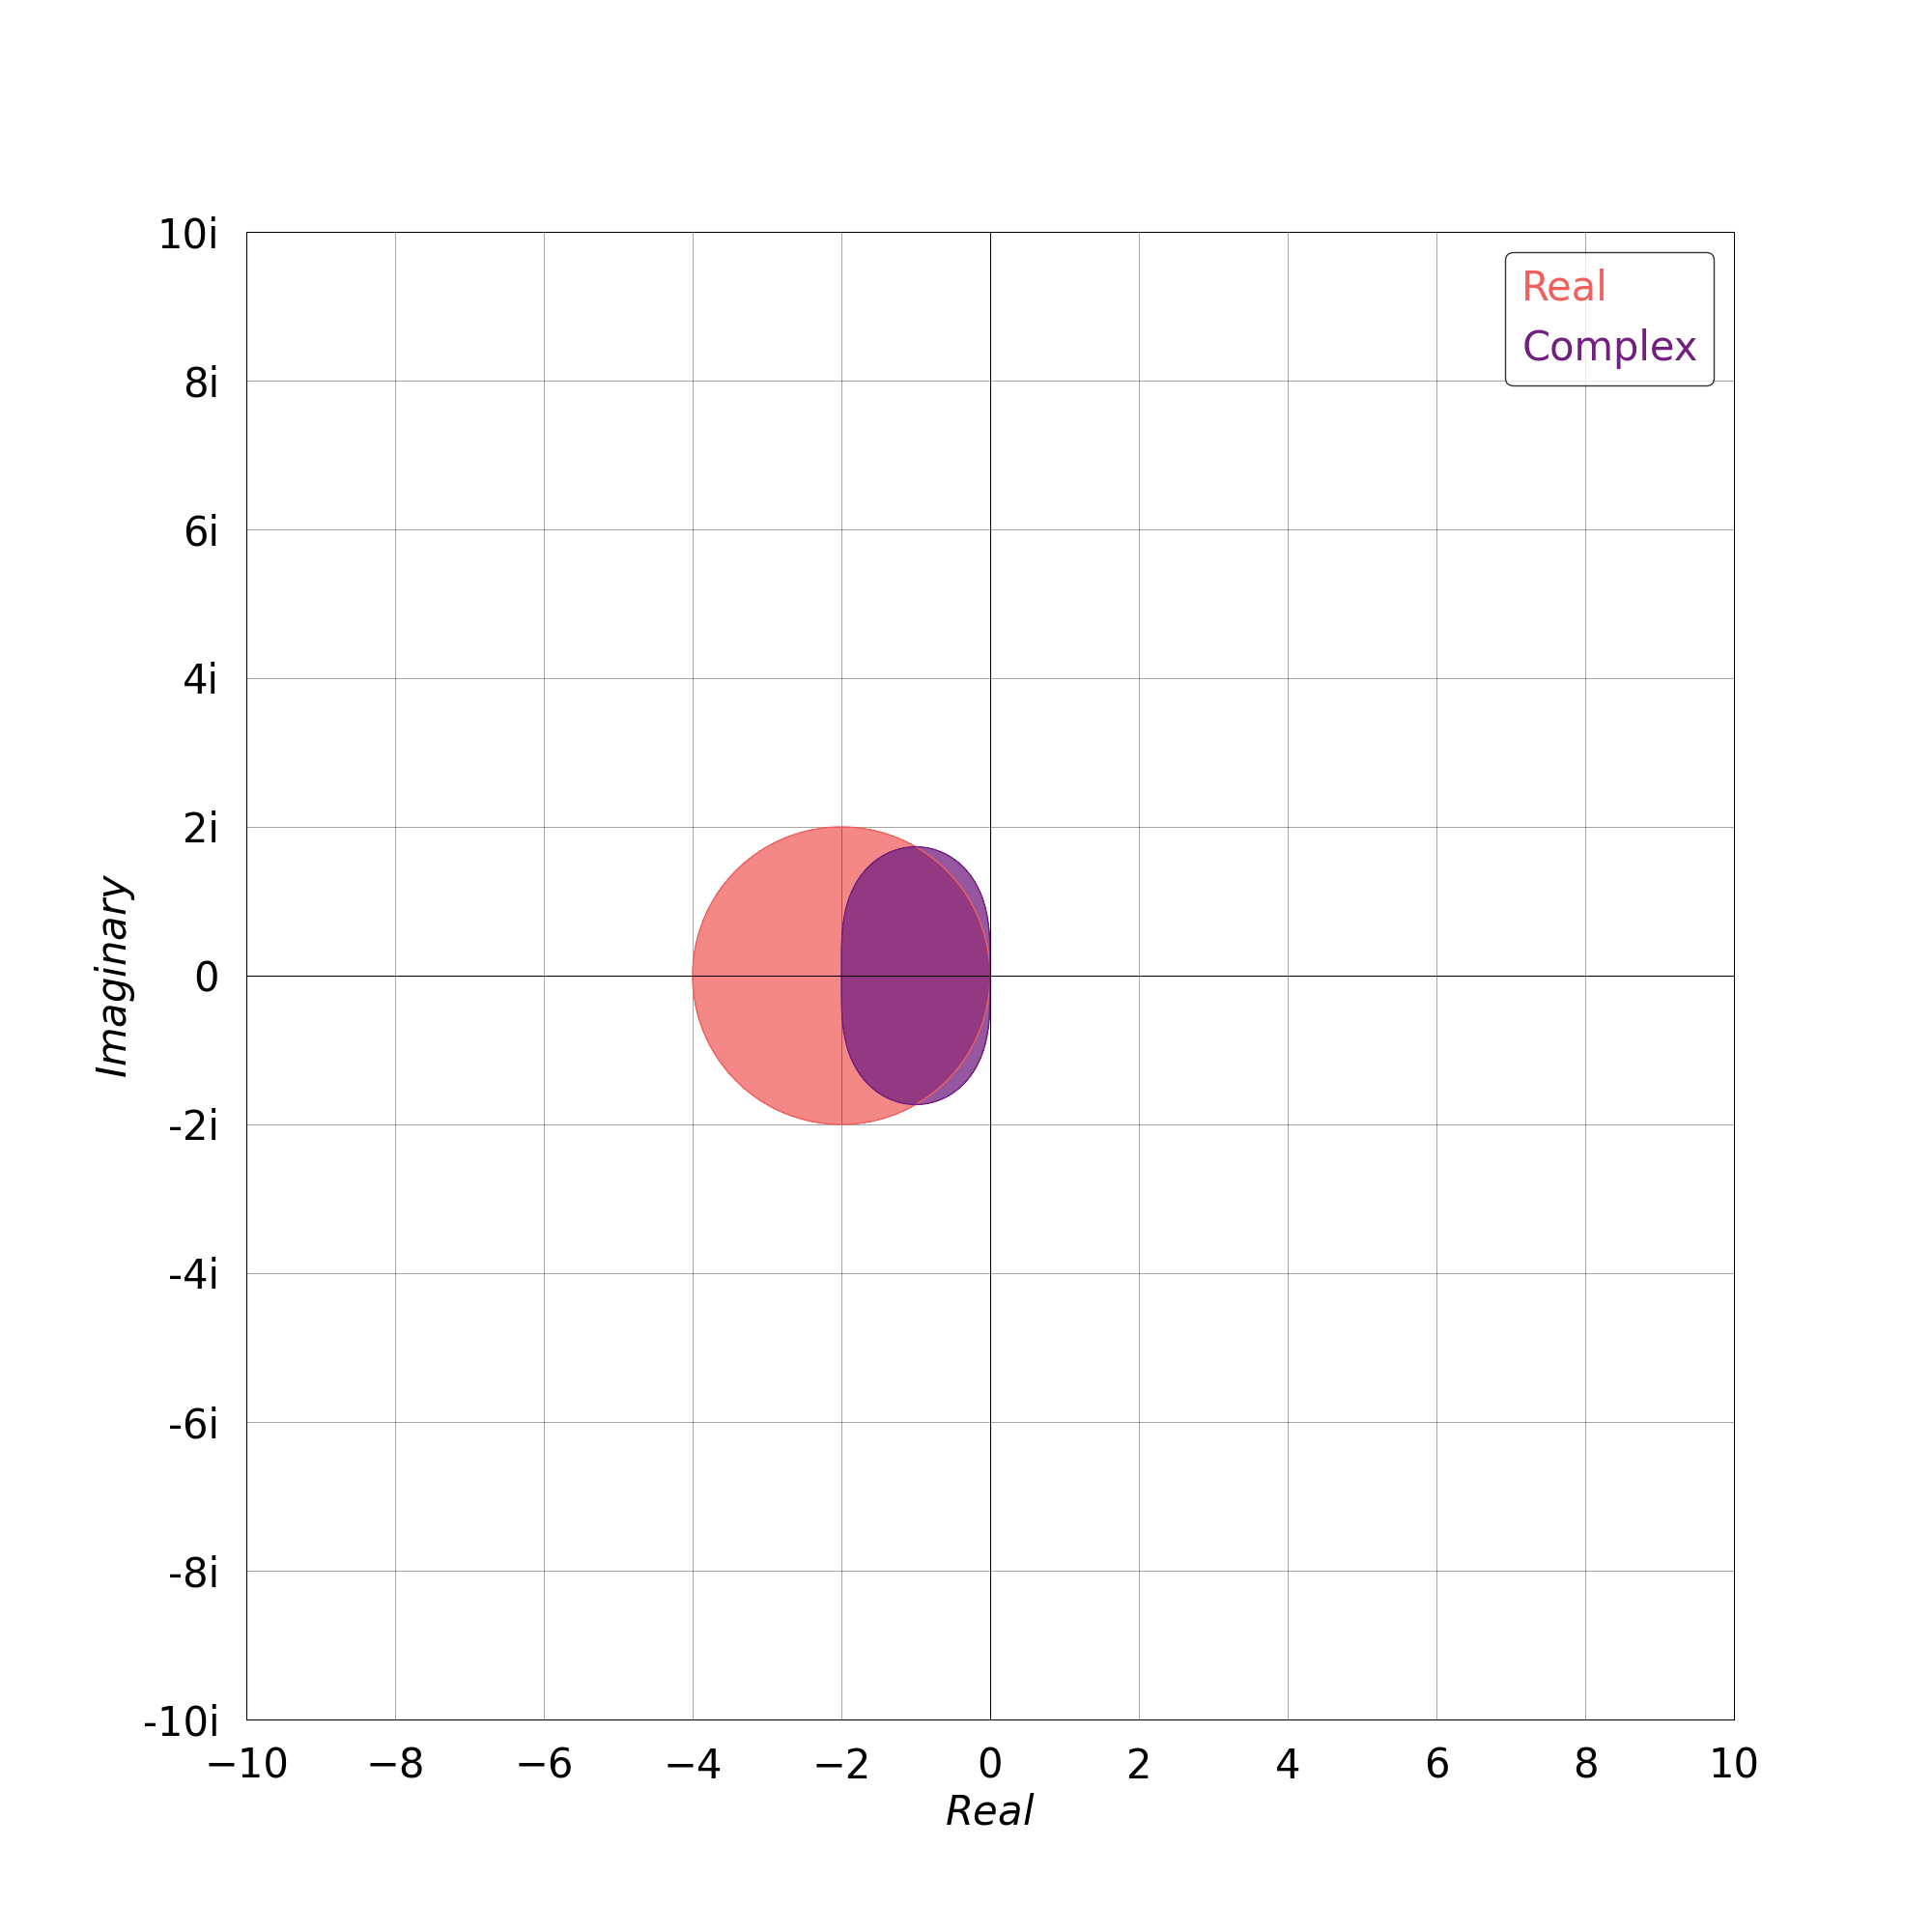
\includegraphics[width=0.49\textwidth]{Stability Regions/Graphs/Real VS Complex Comparison/Euler's Forward.png}
Appendix~\ref{appendix:real_vs_complex_stability} contains the code for this graph.
\end{center}
\columnbreak{}

\textbf{Euler's Forward 2-Step $\bR$}
\begin{flalign*}
	y_{j+1} &= {\Big(1+ \frac{\lh}{2}\Big)}^2 y_j && \\
	\implies &s_{_{\bR}}(\lambda, h) = 1 + \lh + \frac{{(\lh)}^2}{4} &&
\end{flalign*}

\textbf{Euler's Forward 2-Step $\bC$}
\begin{flalign*}
	y_{j+1} &= \Big(1 + z\Big)\Big(1 + \bar{z}\Big) y_j && \\
	    &= \Big(1 + \frac{\lambda h}{2} + bi\Big)\Big(1 + \frac{\lambda h}{2} - bi\Big) y_j && \\
	    &= \bigg(\Big{(1 + \frac{\lambda h}{2}\Big)}^2 + b^2\bigg) y_j && \\
    \implies &s_{_{\mathbb{C}}}(\lambda, h) = 1 + \lambda h + \frac{{(\lambda h)}^2}{4} + b^2 && \\
    \implies &s_{_{\mathbb{C}}}(\lambda, h) = s_{_{\mathbb{R}}}(\lambda, h) + b^2 &&
\end{flalign*}

\vspace*{\fill}
\end{multicols}

\par As $b \in \bR$, $s_{_{\mathbb{C}}}(\lambda, h) \geq s_{_{\mathbb{R}}}(\lambda, h)$\\
This means the stability region for the complex 2-step method is smaller than that of the real 2-step method; there are less values of $\lh$ for which the complex 2-step method is stable.\\
$S_{_{\mathbb{C}}}$ is smaller than $S_{_{\mathbb{R}}}$\\
The diagram above illustrates the case where $b = a = \frac{\lh}{2}$\\
In this case, we have 
\[s_{_{\mathbb{R}}}(\lambda, h) = 1 + \lh + \frac{{(\lambda h)}^2}{4} = M(y) + \mathcal{O}({(\lh)}^2)\]
while
\[s_{_{\mathbb{C}}}(\lambda, h) = 1 + \lh + \frac{{(\lambda h)}^2}{2} = M(y) + \mathcal{O}({(\lh)}^3)\]
The complex 2-step method has a higher order of accuracy than the real 2-step method, with the trade-off of a smaller stability region.\\

\par We can do the same kind of analysis for other Numerical Methods.\\
The same derivations and diagrams for the Backward Euler and Runge-Kutta 4 methods follow.\\

\subsubsection{Euler's Backward 2-Step}
\begin{theorem}\textbf{Euler's Backward Complex Step Pairs must be Conjugate for $\lambda \in \bR$}\\
\par For the exponential decay problem, $y=e^{\lambda t}$, let $\lambda \in \bR$\\
Let $z_1 = a_1 + b_1i$ and $z_2 = a_2 + b_2i$ be a complex step pair for Euler's Backward 2-Step Method.\\
Then we must have $z_2 = \bar{z_1}$\\
\par\textbf{Proof:}
\[\lambda \in \bR \implies y_{j}, y_{j+1} \in \bR\]
Euler's Backward 2-Step Method is given by:
\begin{flalign*}
	y_{j+1} &= s(\lambda, z_1) s(\lambda, z_2)\; y_j && \\
	&= \Big(\frac{1}{1-z_1}\Big)\Big(\frac{1}{1-z_2}\Big)\; y_j && \\
        &= \Big(\frac{1}{(1-z_1)(1-z_2)}\Big)\; y_j &&
\end{flalign*}
\begin{flalign*}
	(1-z_1)(1-z_2) &= (1-a_1-b_1i)(1-a_2-b_2i) &&\\
		       &= \big[1-a_1-a_2+a_1 a_2-b_1 b_2\big] + \big[a_1 b_2 + a_2 b_1 - b_1 - b_2\big]i && \\
		       &= \big[(a_1-1)(a_2-1)-b_1 b_2\big] + \big[b_1(a_2-1) + b_2(a_1-1)\big]i && 
\end{flalign*}
\[y_{j+1} \in \bR \implies Im(y_{j+1}) = 0 \implies b_1(a_2-1) + b_2(a_1-1) = 0\]
\[z_1+z_2 = h \in \bR \implies a_1+a_2 + (b_1+b_2)i = h \implies b_1+b_2 = 0 \implies b_1 = -b_2\]
\[b_1(a_2-1) + b_2(a_1-1) = 0 \implies b_1(a_2-1) - b_1(a_1-1) = 0 \implies b_1 = 0 = b_2 \text{ or } a_1 = a_2\]
Thus, $z_1, z_2 \in \bC \implies a_1 = a_2$ and $b_1 = -b_2$
\[\therefore z_1 = a_1 + b_1i \text{ and } z_2 = a_1 - b_1i \implies z_2 = \bar{z_1} \qquad\square\]
\end{theorem}
\begin{multicols}{2}
\begin{center}
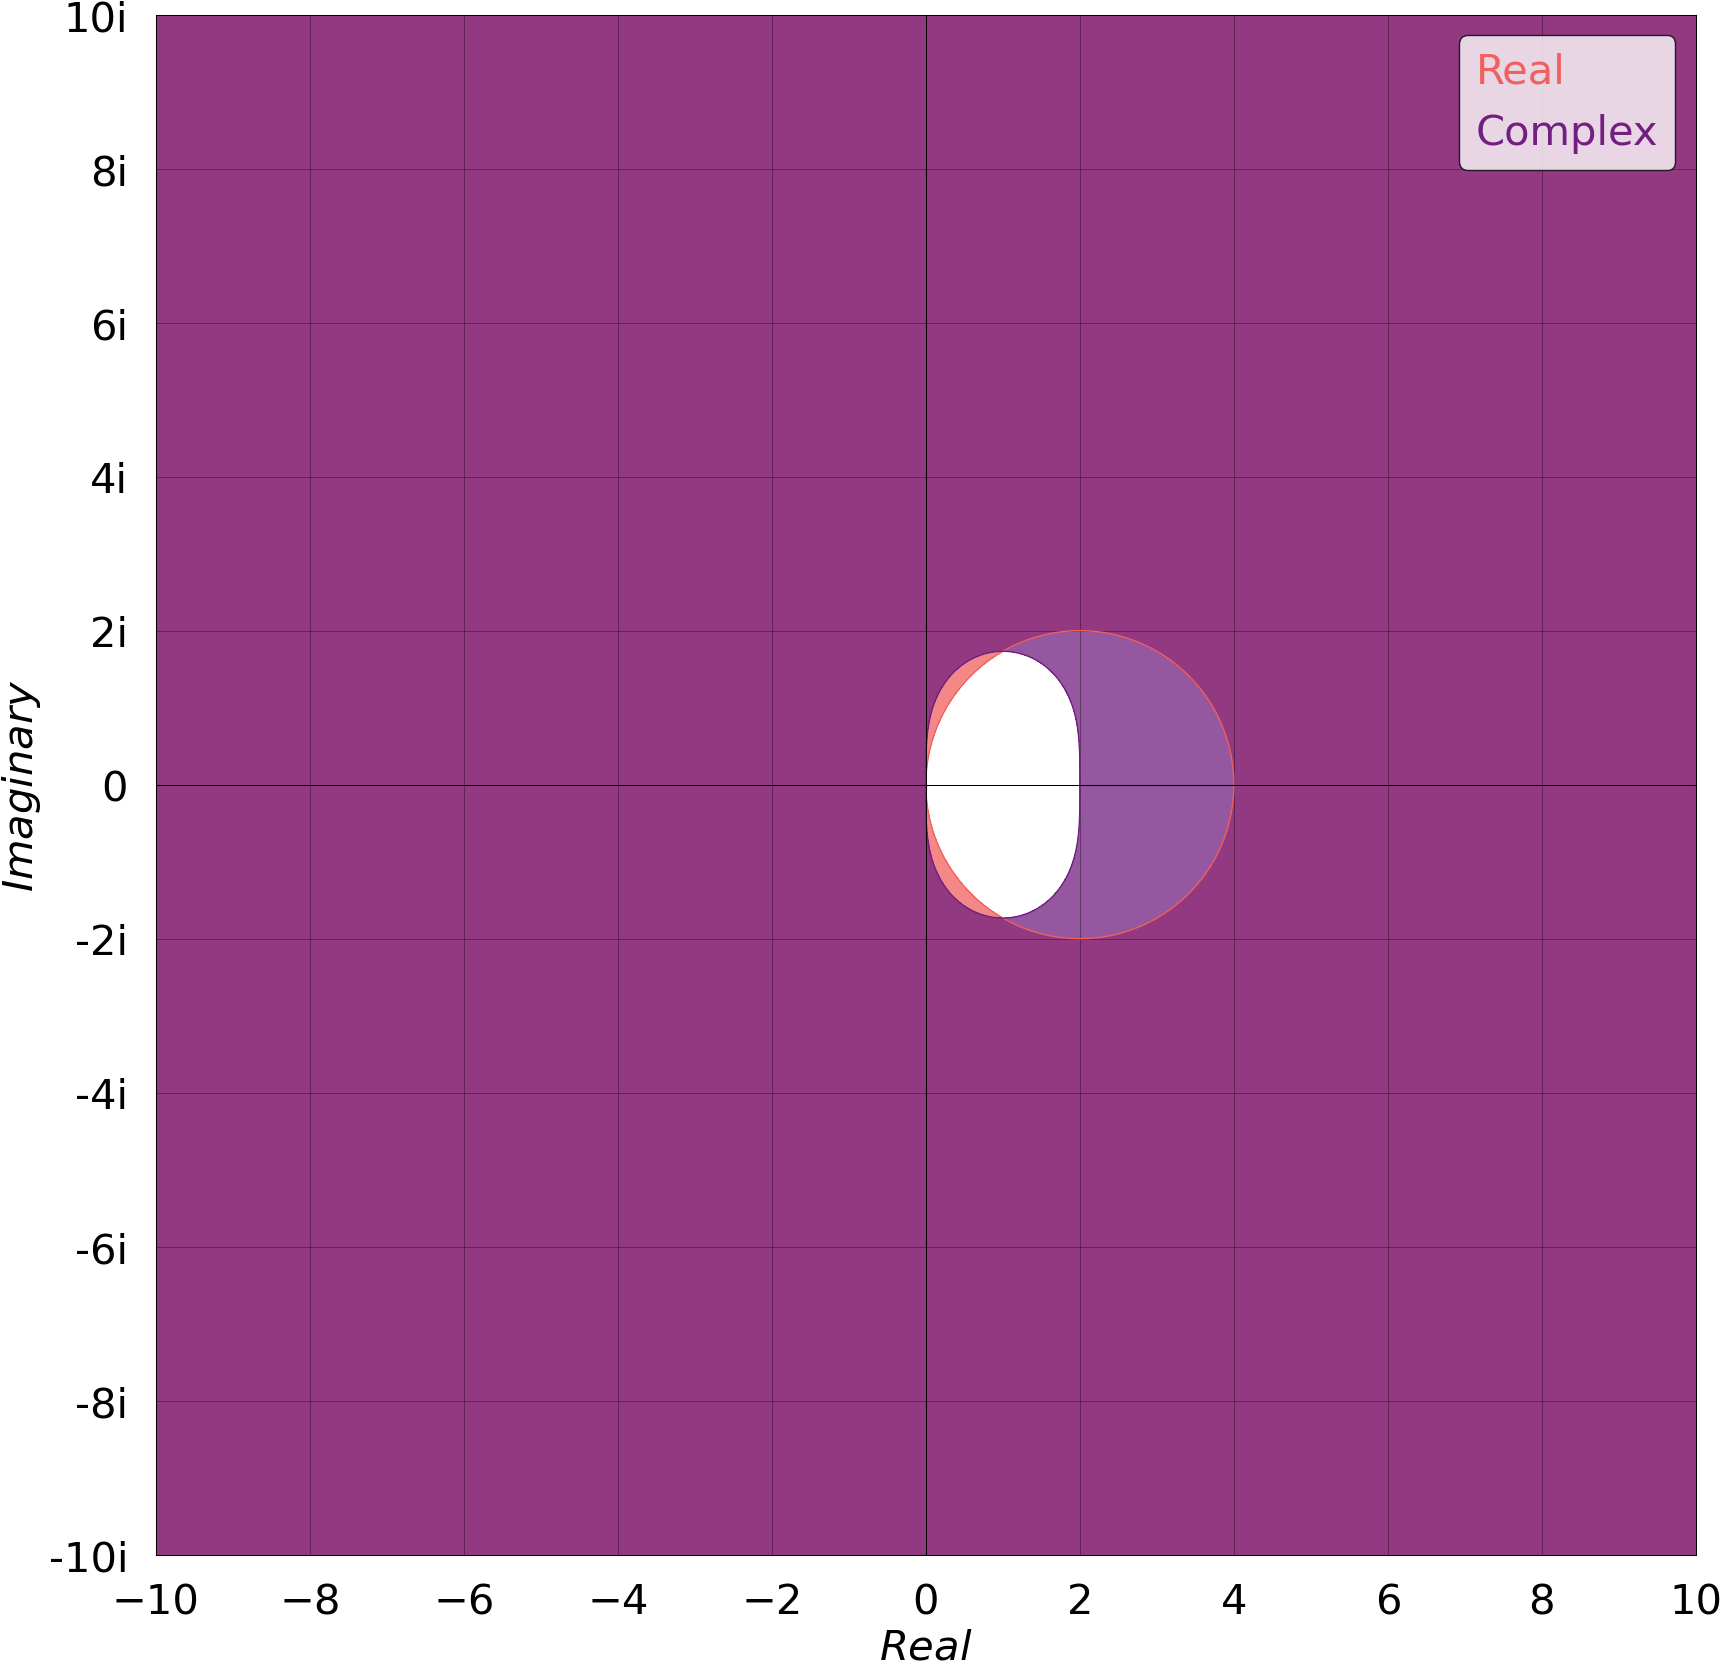
\includegraphics[width=0.49\textwidth]{Stability Regions/Graphs/Real VS Complex Comparison/Euler's Backward.png}
Appendix~\ref{appendix:real_vs_complex_stability} contains the code for this graph.
\end{center}
\columnbreak{}

\textbf{Euler's Backward 2-Step $\bR$}
\begin{flalign*}
	y_{j+1} &= {\bigg(\frac{1}{1-\frac{\lh}{2}}\bigg)}^2 y_j && \\
	\implies & s_{\bR}(\lambda, h) = \frac{1}{1 - \lh + \frac{{(\lh)}^2}{4}} &&
\end{flalign*}

\textbf{Euler's Backward 2-Step $\bC$}
\begin{flalign*}
	y_{j+1} &= \bigg(\frac{1}{1-\frac{\lh}{2}+bi}\bigg)\bigg(\frac{1}{1-\frac{\lh}{2}-bi}\bigg)y_j && \\
    \implies &s_{\bC}(\lambda, h) = \frac{1}{1 - \lh + \frac{{(\lh)}^2}{4} + b^2} && \\
\end{flalign*}
\par Again, $b \in \bR$, so this time,\\
$s_{_{\mathbb{C}}}(\lambda, h) \leq s_{_{\mathbb{R}}}(\lambda, h) \implies S_{_{\mathbb{C}}}$ is larger than $S_{_{\mathbb{R}}}$\\
\vspace*{\fill}
\end{multicols}

\newpage
\subsubsection{Runge-Kutta 4 2-Step}
\begin{conjecture}\textbf{Runge-Kutta 4 Complex Step Pairs must be Conjugate for $\lambda \in \bR$}\\
	\par This is left as a conjecture for now, as the expansion we did in the other two proofs is much more complicated for the Runge-Kutta 4 method.\\
	The proof is left as an exercise in futility for the reader.\\
	Have a look at Appendix~\ref{appendix:rk4_conjecture} for the full expansion of the stability function for the Runge-Kutta 4 method,\\
	if long algebraic expressions are your flavour of masochism.\\
\end{conjecture}
\begin{multicols}{2}
\begin{center}
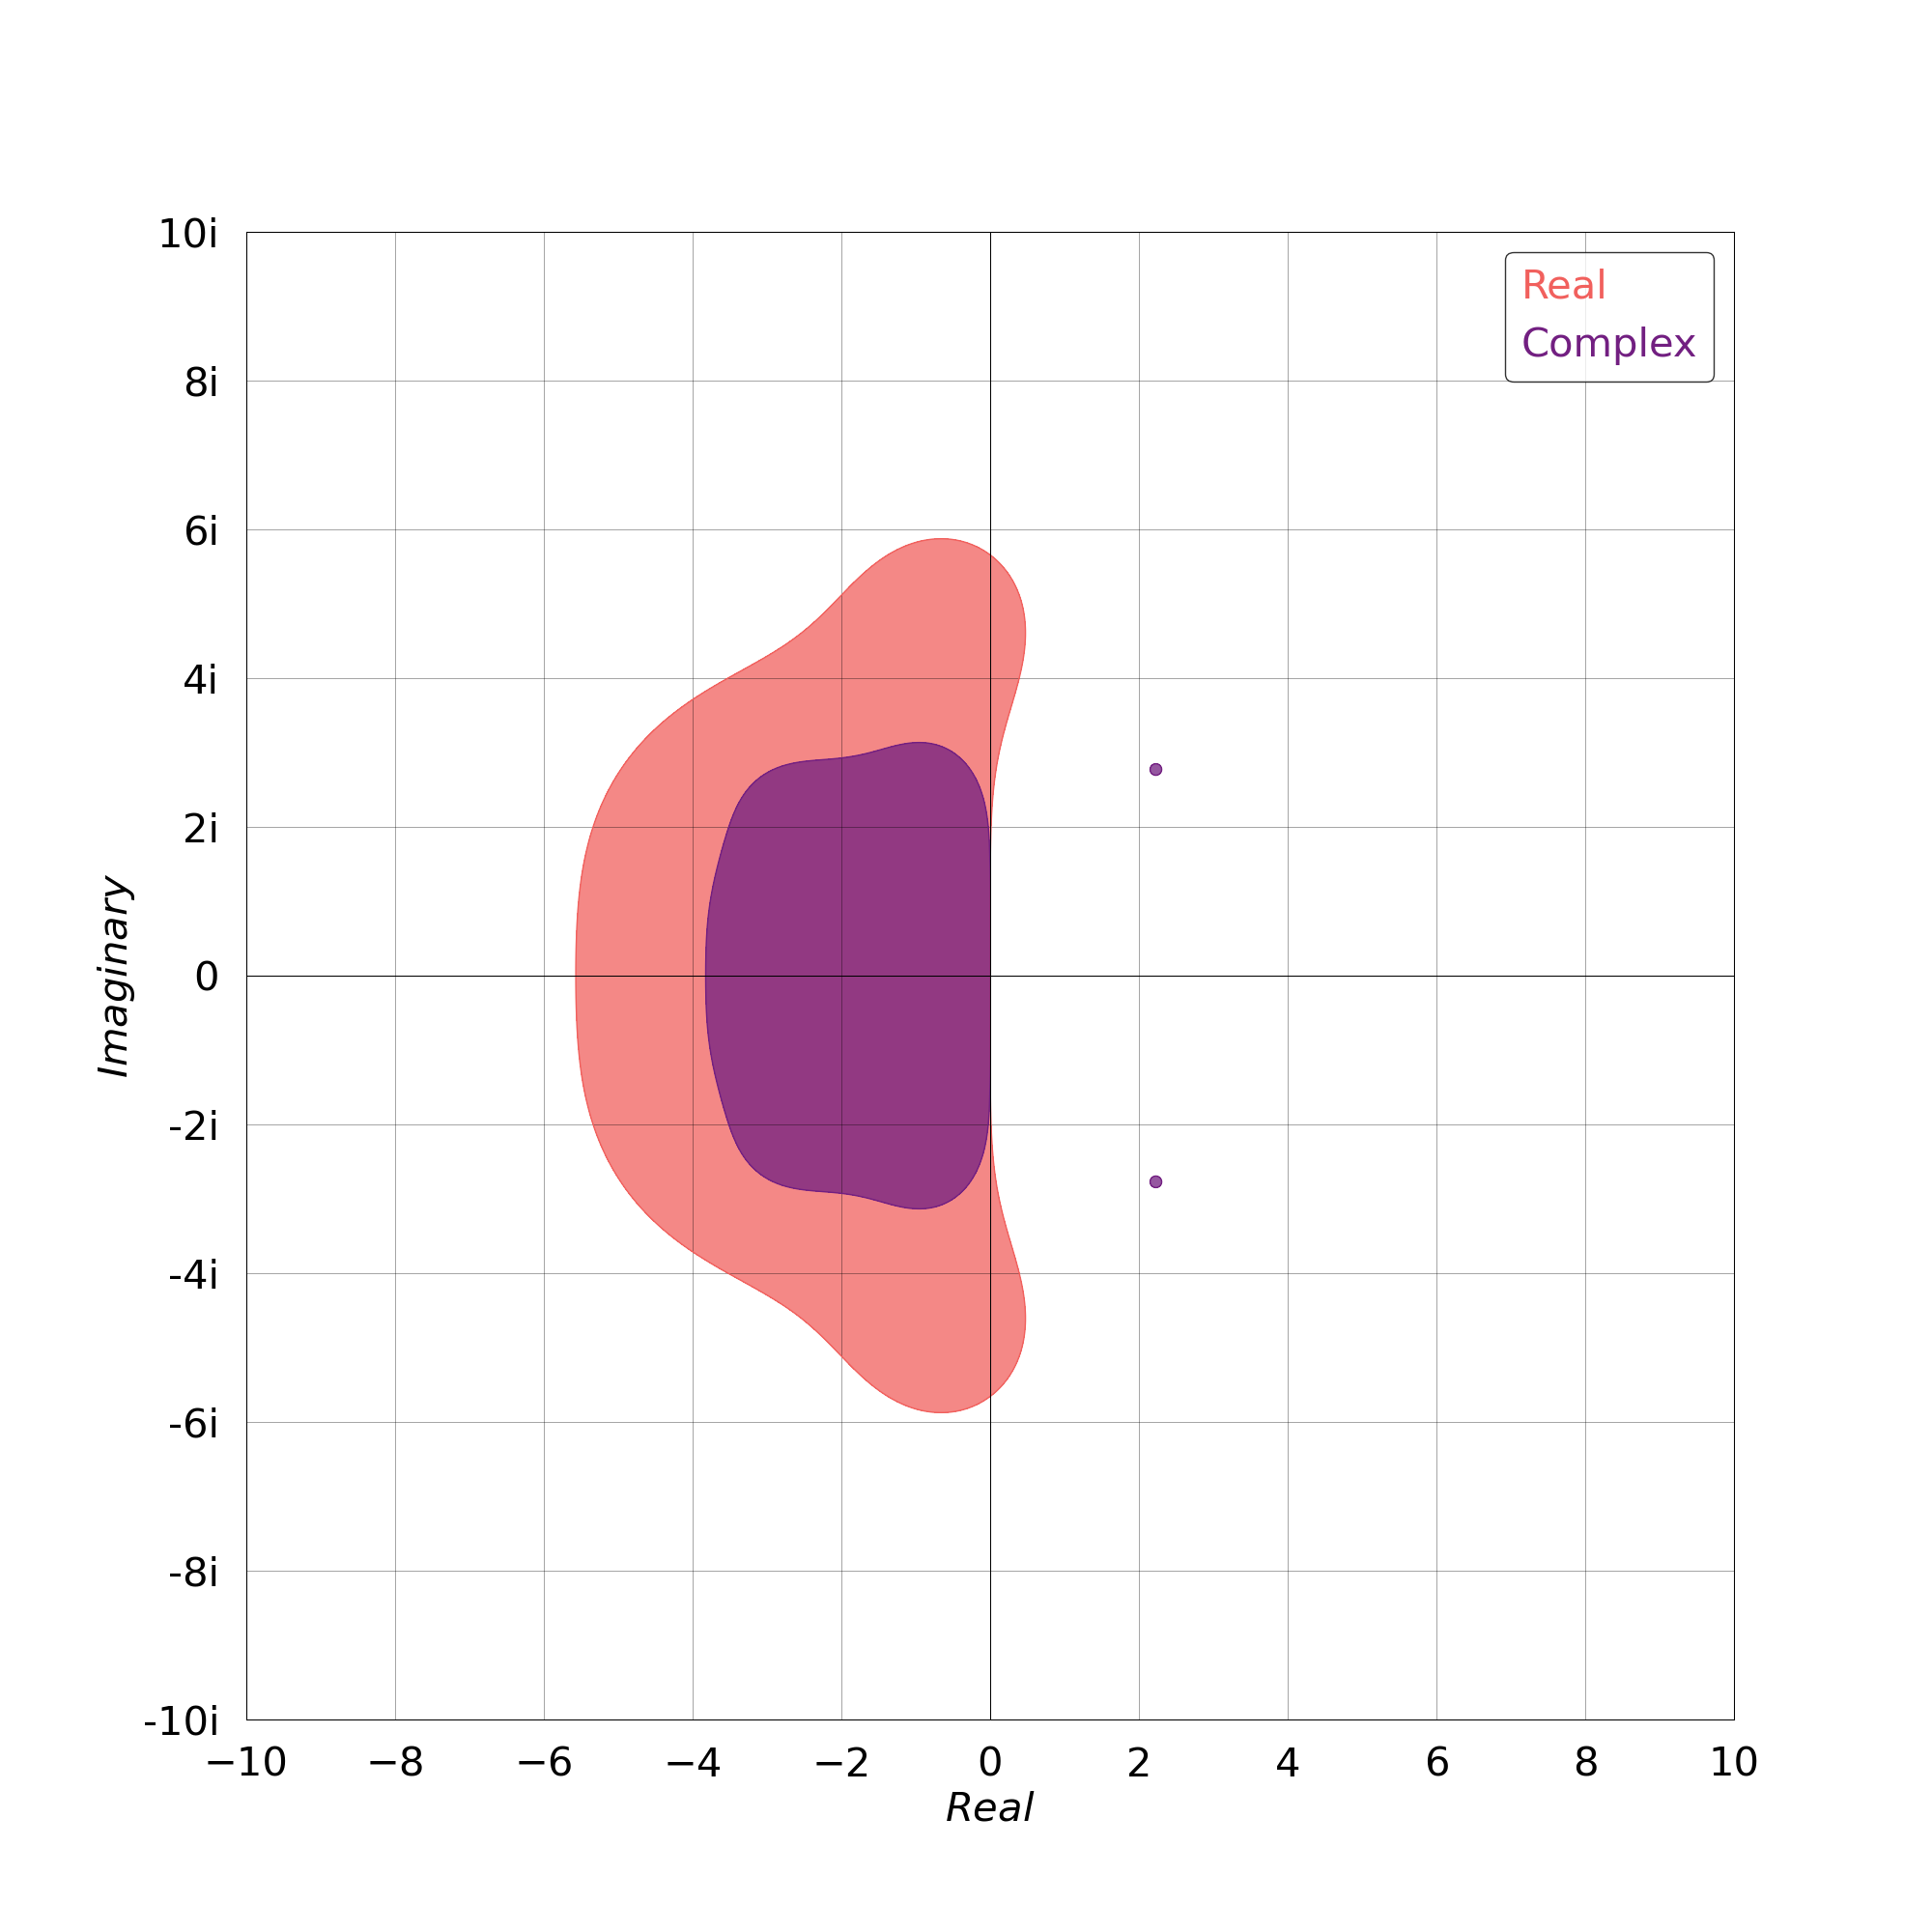
\includegraphics[width=0.49\textwidth]{Stability Regions/Graphs/Real VS Complex Comparison/Runge-Kutta 4.png}
Appendix~\ref{appendix:real_vs_complex_stability} contains the code for this graph.
\end{center}
\columnbreak{}

\textbf{Runge-Kutta 4 2-Step $\bR$}
\begin{flalign*} 
	y_{j+1} &= {\bigg(1+\frac{\lh}{2}+\frac{{(\frac{\lh}{2})}^2}{2}+\frac{{(\frac{\lh}{2})}^3}{6}+\frac{{(\frac{\lh}{2})}^4}{24}\bigg)}^2 y_j && \\
	y_{j+1} &= \bigg(1+\lh+\frac{{(\lh)}^2}{2}+\frac{{(\lh)}^3}{6}+\frac{{(\lh)}^4}{24} && \\
            &\quad\,\,\,\,+\frac{{(\lh)}^5}{128}+\frac{5{(\lh)}^6}{4608}+\frac{{(\lh)}^7}{9216}+\frac{{(\lh)}^8}{147456}\bigg) y_j && \\
	\implies &s_{_{\bR}}(\lambda, h) = 1+\lh+\frac{{(\lh)}^2}{2}+\frac{{(\lh)}^3}{6}+\frac{{(\lh)}^4}{24} && \\
            &\qquad\qquad\quad+\frac{{(\lh)}^5}{128}+\frac{5{(\lh)}^6}{4608}+\frac{{(\lh)}^7}{9216}+\frac{{(\lh)}^8}{147456} &&
\end{flalign*}

\textbf{Runge-Kutta 4 2-Step $\bC$}
\[y_{j+1} = \bigg(1+z+\frac{z^2}{2}+\frac{z^3}{6}+\frac{z^4}{24}\bigg)\bigg(1+\bar{z}+\frac{\bar{z}^2}{2}+\frac{\bar{z}^3}{6}+\frac{\bar{z}^4}{24}\bigg) y_j\]

\end{multicols}
$\implies s_{_{\bC}}(\lambda, h) = 1 + \lh + \frac{\lh^2}{2} + \frac{\lh^3}{6} + \frac{\lh^4}{24} + \frac{\lh^5}{128} + \frac{5 \lh^6}{4608} + \frac{\lh^7}{9216} + \frac{\lh^8}{147456} + \frac{b^2 \lh^3}{48} + \frac{b^2 \lh^4}{128} + \frac{b^2 \lh^5}{768} + \frac{b^2 \lh^6}{9216} + \frac{b^4 \lh}{24} - \frac{b^4 \lh^2}{96} + \frac{b^4 \lh^3}{192} + \frac{b^4 \lh^4}{1536} - \frac{b^6}{72} + \frac{b^6 \lh}{144} + \frac{b^6 \lh^2}{576} + \frac{b^8}{576}$
\newpage
\subsection{Varying b for Complex Conjugate Step Pairs}
\par As mentioned earlier, we need not only focus on the case where $b = \frac{\lh}{2}$\\
We can vary $b$ and see how the stability regions change.\\
In the cases below, we have preserved $a = \frac{\lh}{2}$\\
Consequently, these are still complex conjugate step pairs.\\
Videos showing the stability regions for varying $b$ values can be found in the \textit{GitHub Repository}\cite{GitHub_Repo} for this project.\\
These videos were created frame-by-frame using the script in Appendix~\ref{appendix:video_frames}.\\
The frames were stiched together using the script in Appendix~\ref{appendix:frames_to_video}.\\
Below are some of the video frames for each method.\\
\textbf{Observations:}
\begin{itemize}
	\item[$\cdot$] The stability region for complex conjugate pairs is always symmetric accross the real axis.
	      
	\item[$\cdot$] As $b$ increases, the stability region shrinks for explicit methods and grows for implicit methods.\\
        This can be seen quite simply in the $s_{_{\bC}}(\lambda, h)$ equations for Euler's Forward and Backward methods.

        \item[$\cdot$] The stability region for Euler's Backward Method is the complement of that for Euler's Forward Method, after it has been reflected across the imaginary axis.

\end{itemize}
\subsubsection{Euler's Forward}
\vspace*{-0.65cm}
\begin{multicols}{3}
	\begin{center}
		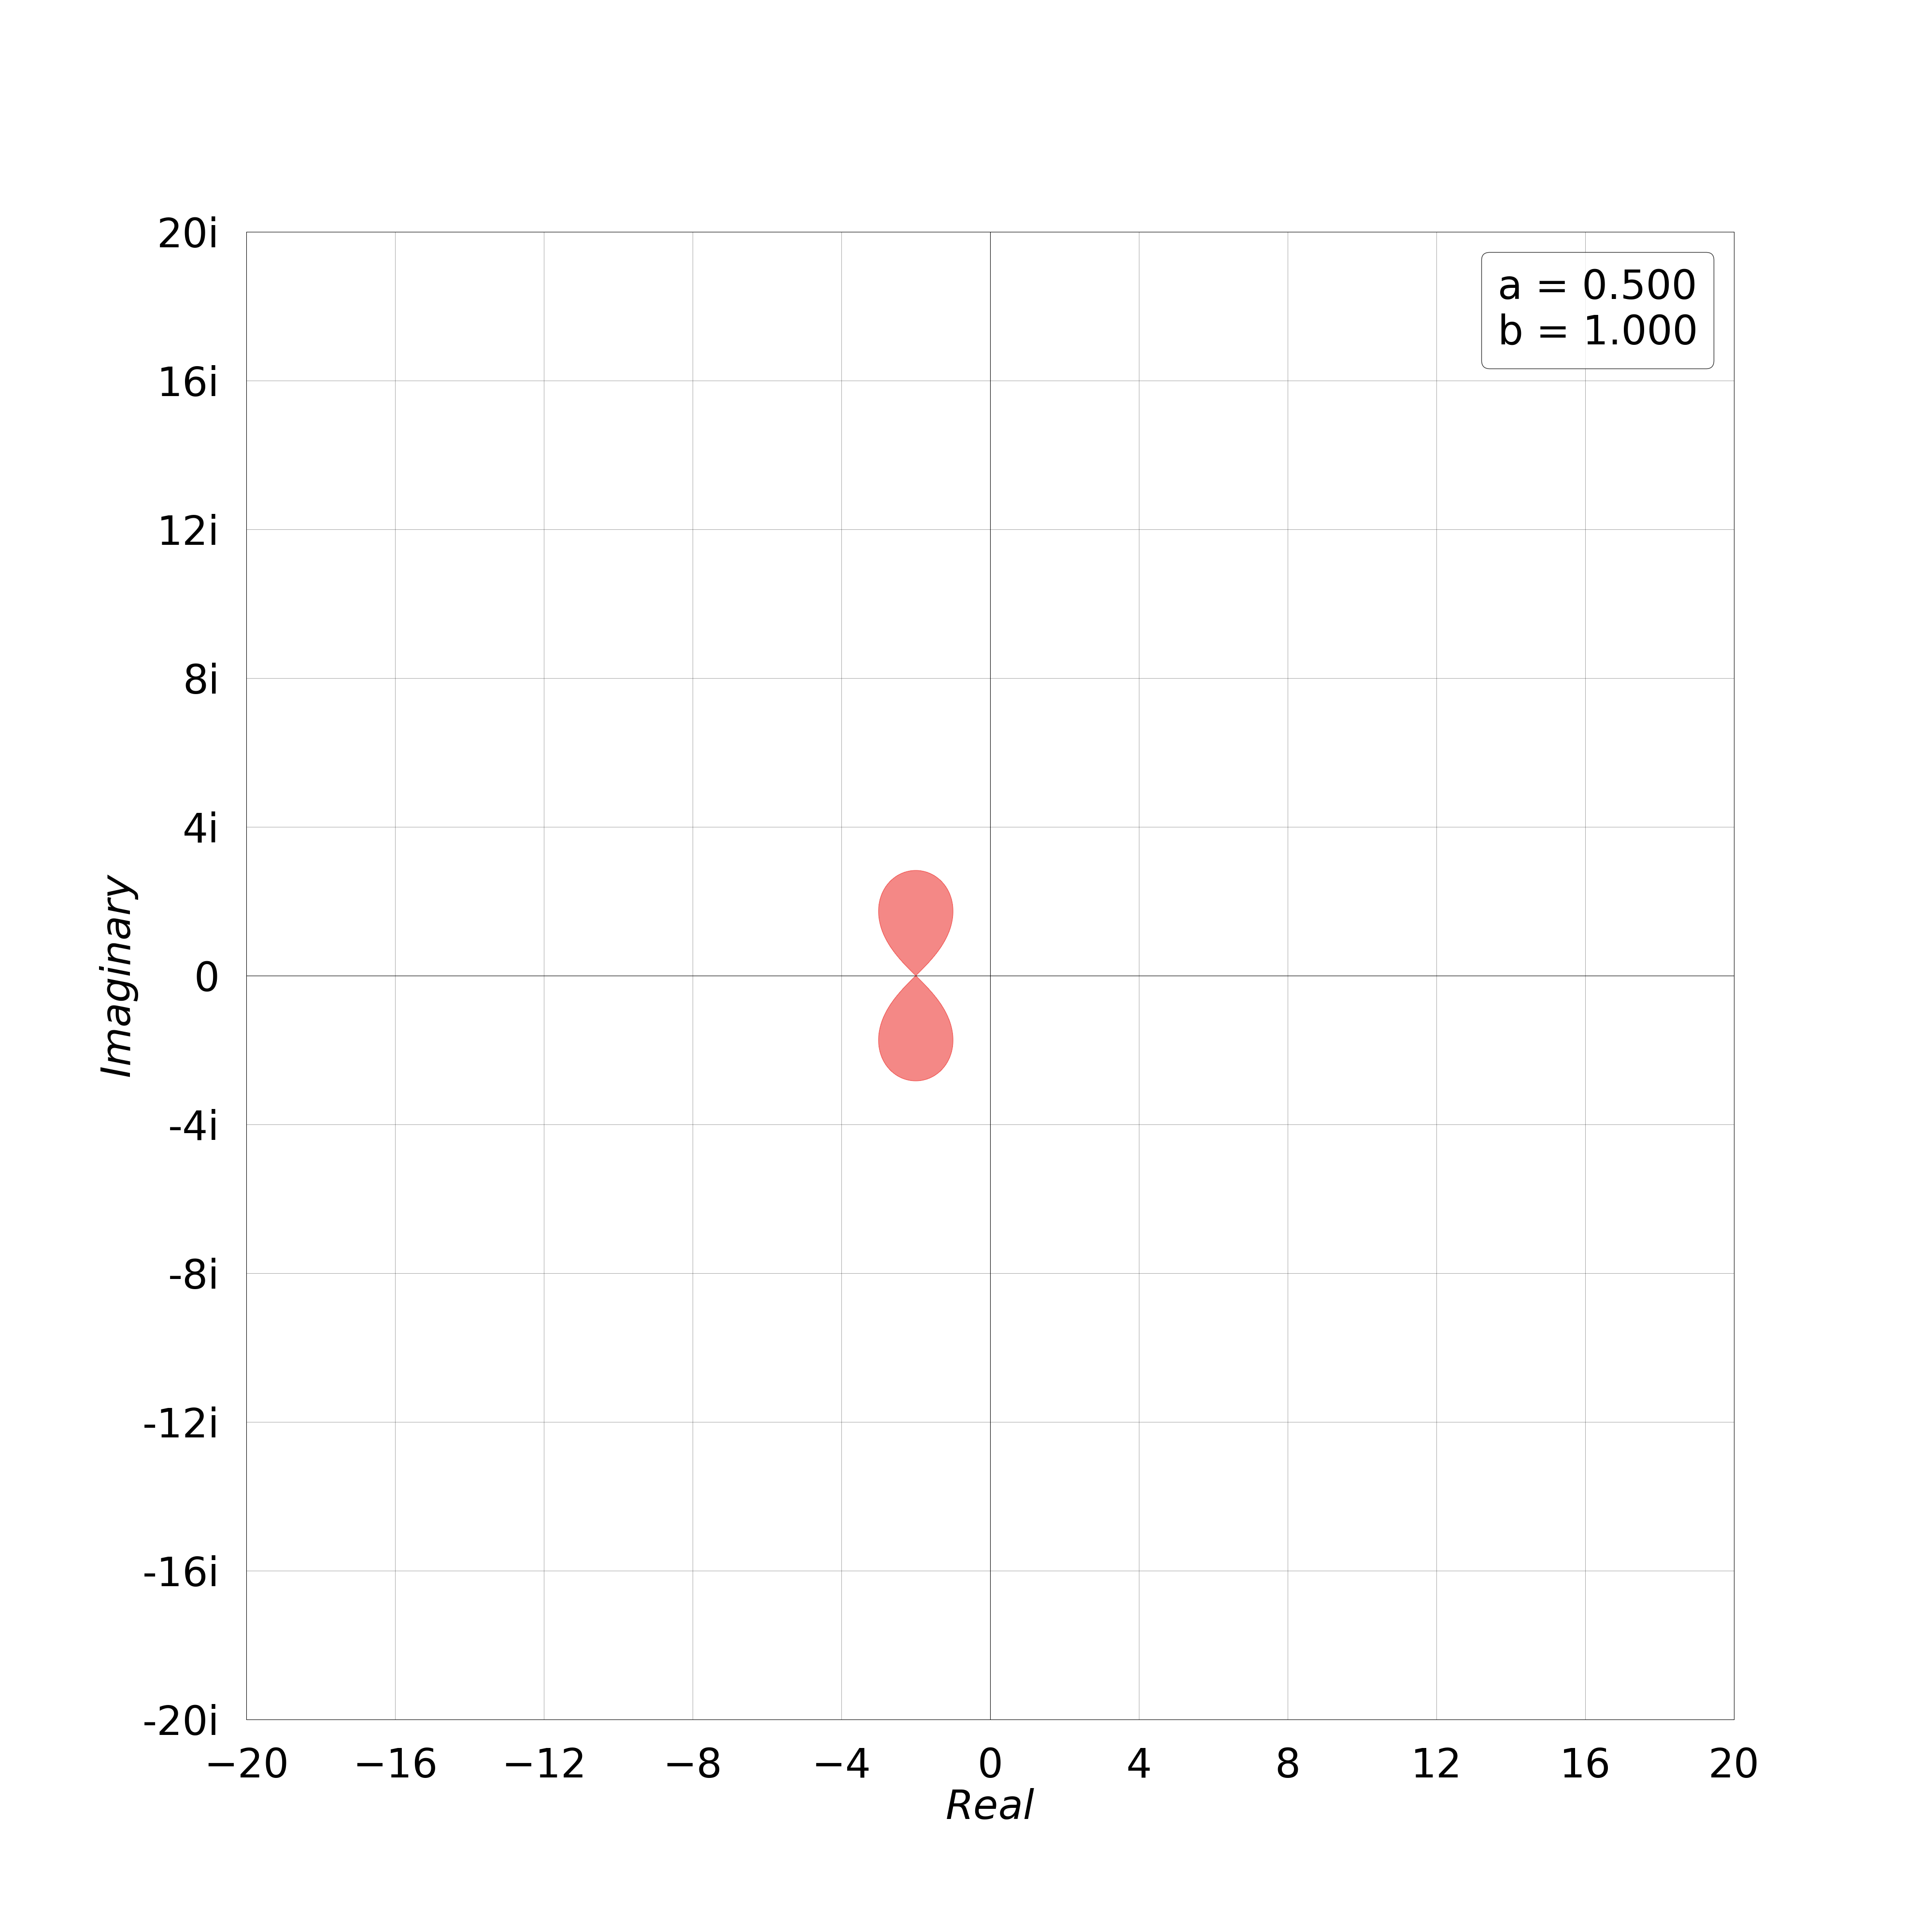
\includegraphics[width=0.32\textwidth]{Stability Regions/Videos/Varied b/Euler's Forward/a=0.5/frames/0200.png}
	\end{center}
	\columnbreak{}
	\begin{center}
		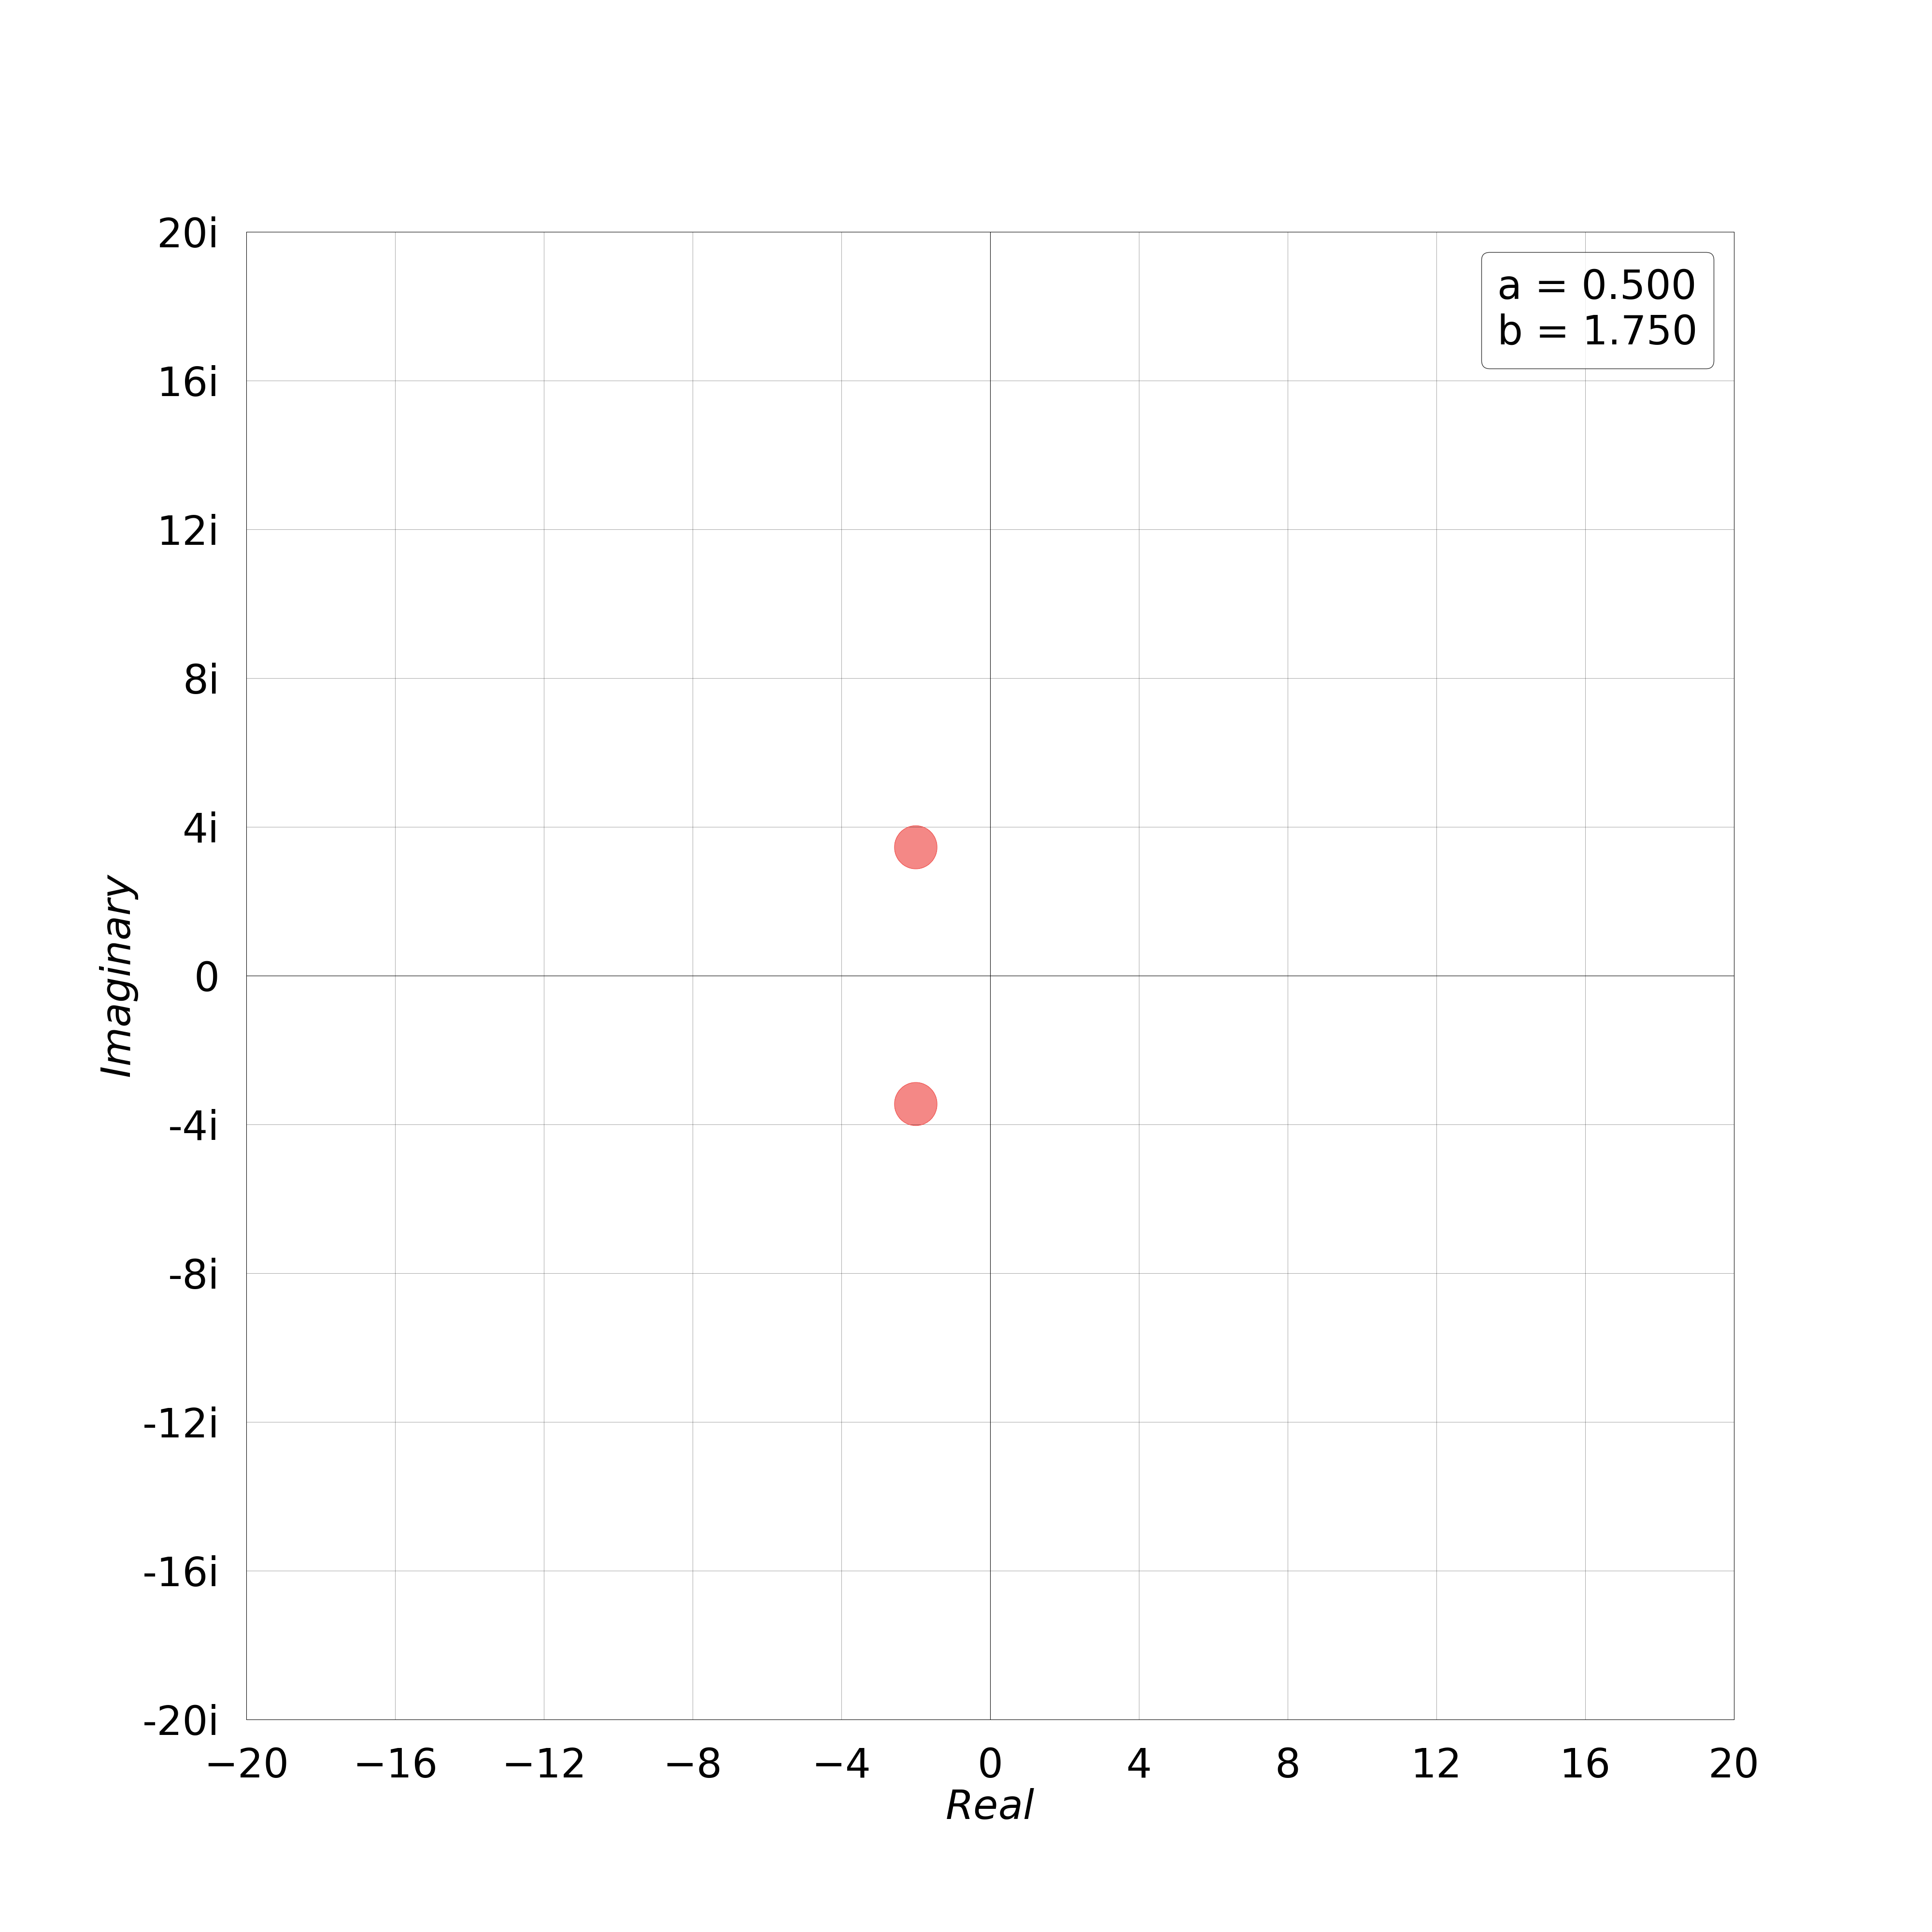
\includegraphics[width=0.32\textwidth]{Stability Regions/Videos/Varied b/Euler's Forward/a=0.5/frames/0350.png}
	\end{center}
	\columnbreak{}
	\begin{center}
		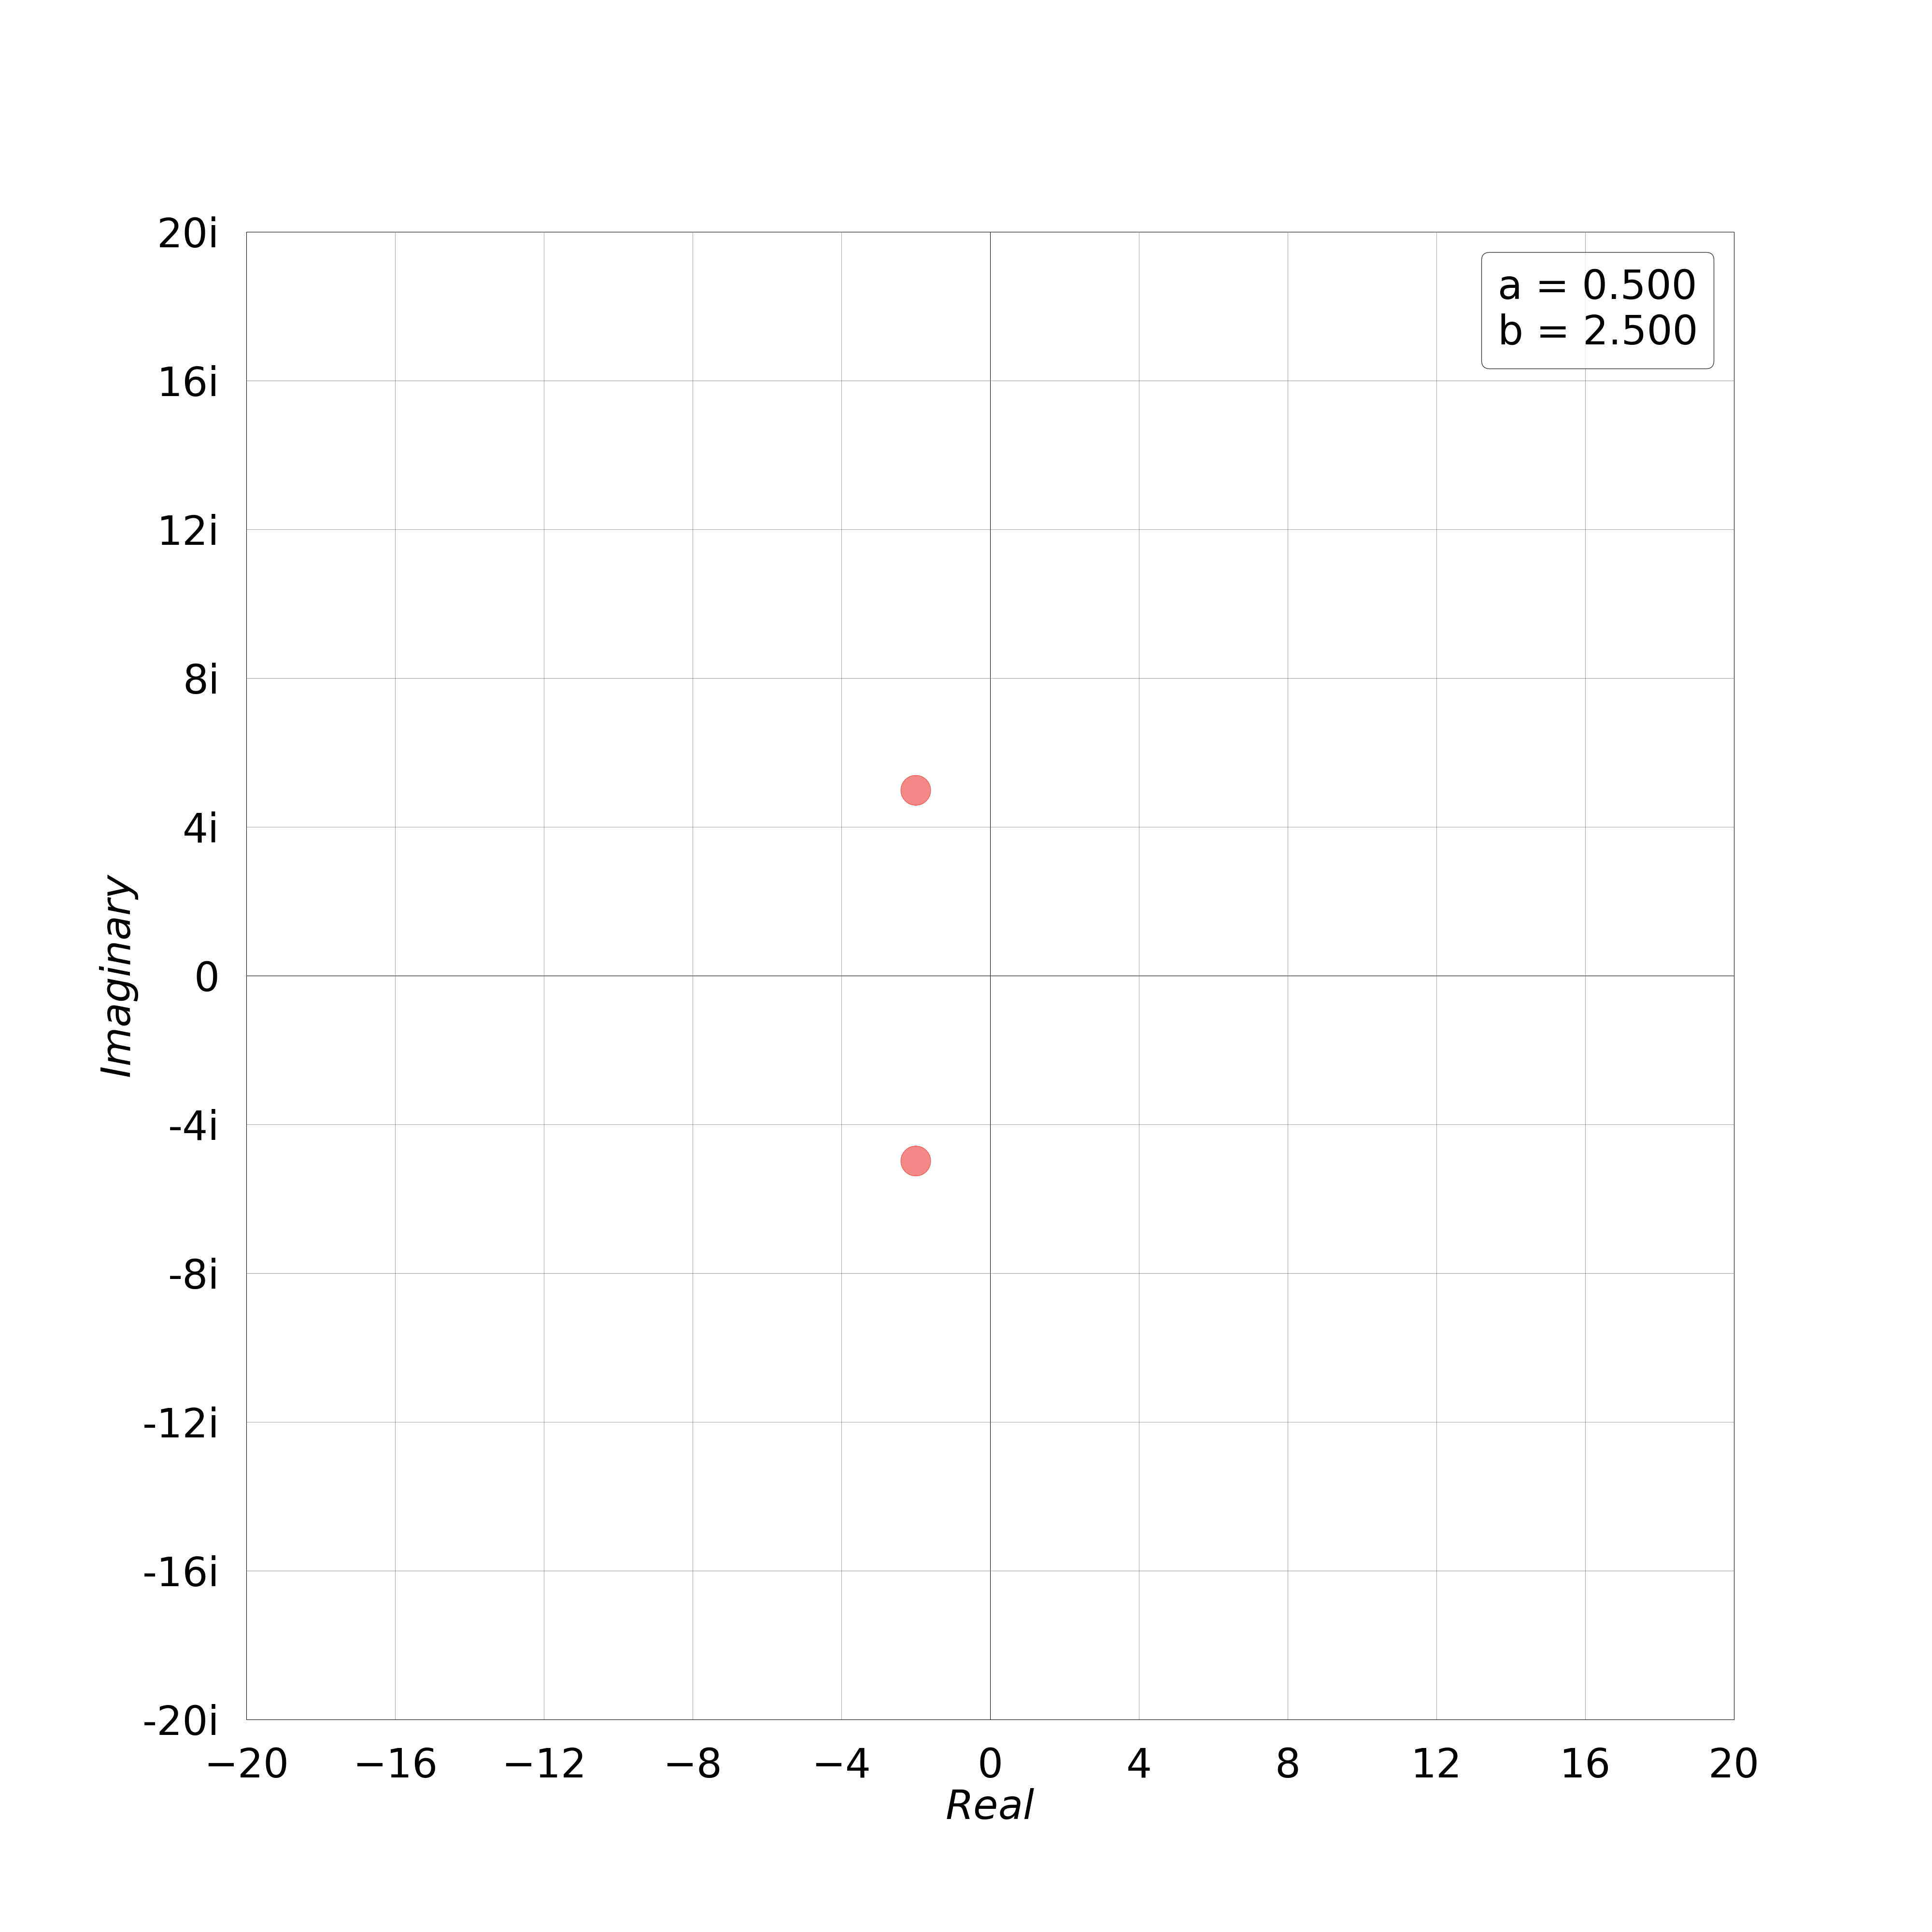
\includegraphics[width=0.32\textwidth]{Stability Regions/Videos/Varied b/Euler's Forward/a=0.5/frames/0500.png}
	\end{center}
\end{multicols}
\subsubsection{Euler's Backward}
\vspace*{-0.65cm}
\begin{multicols}{3}
	\begin{center}
		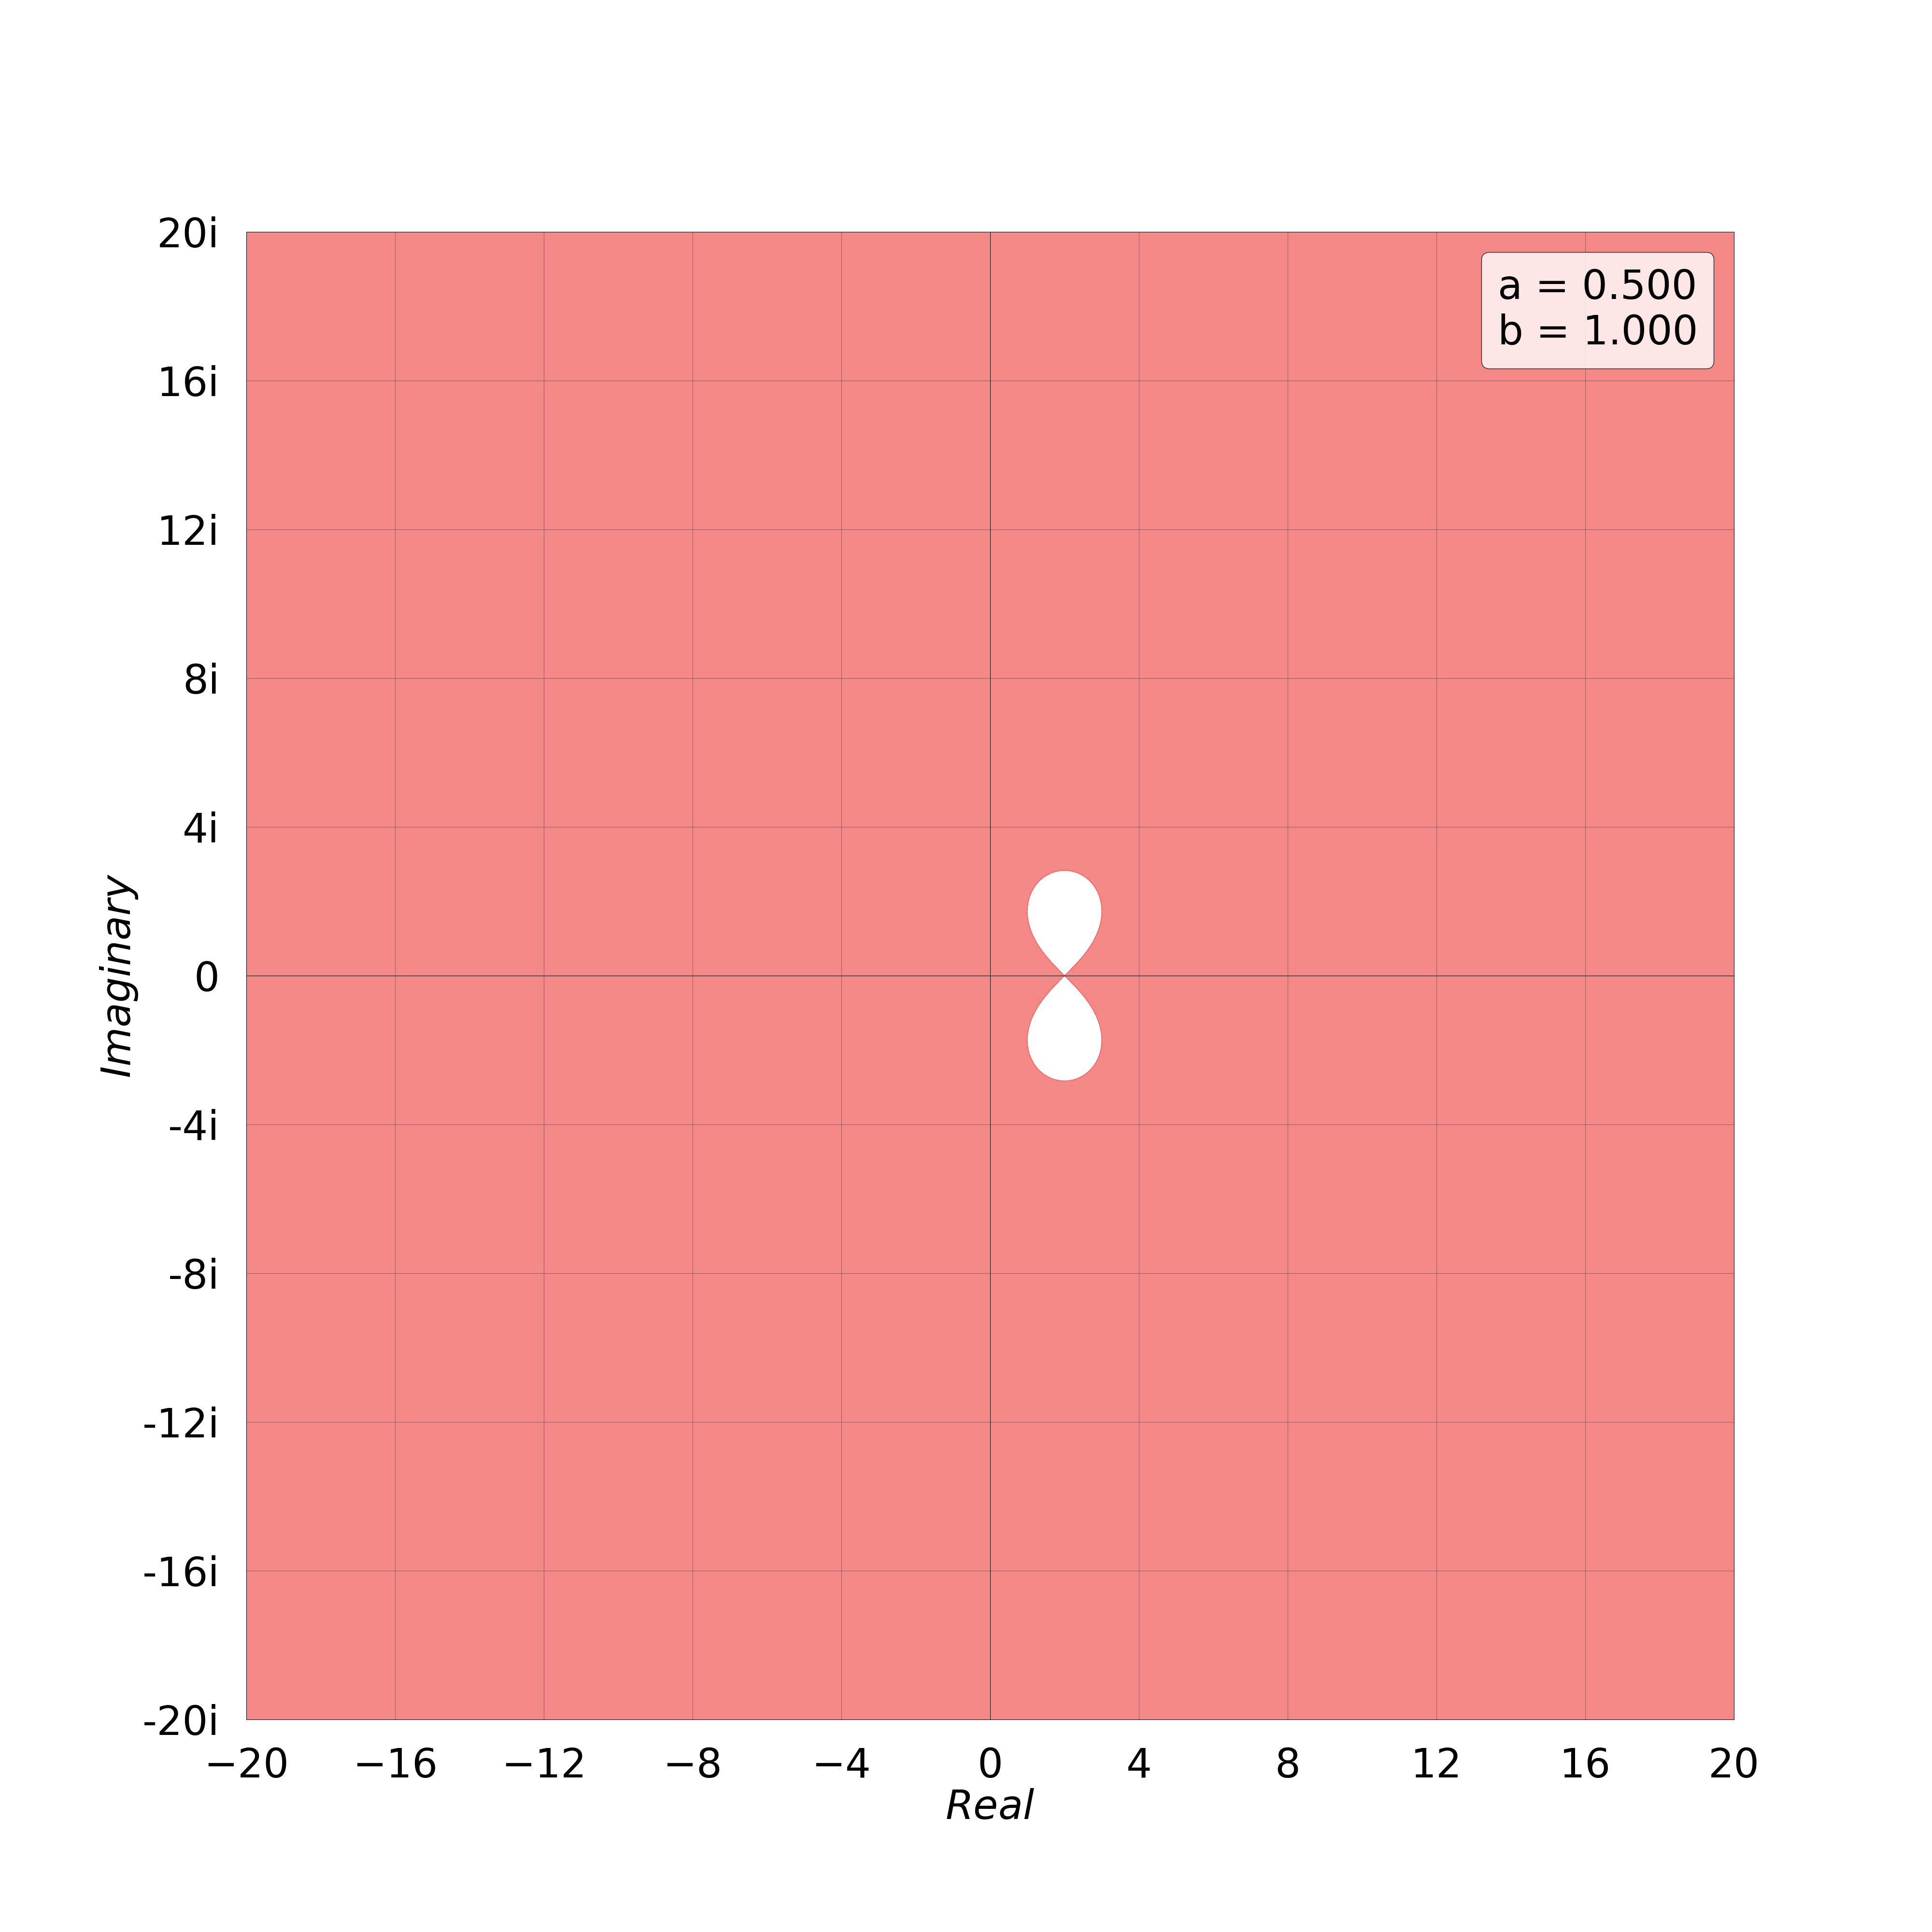
\includegraphics[width=0.32\textwidth]{Stability Regions/Videos/Varied b/Euler's Backward/a=0.5/frames/0200.png}
	\end{center}
	\columnbreak{}
	\begin{center}
		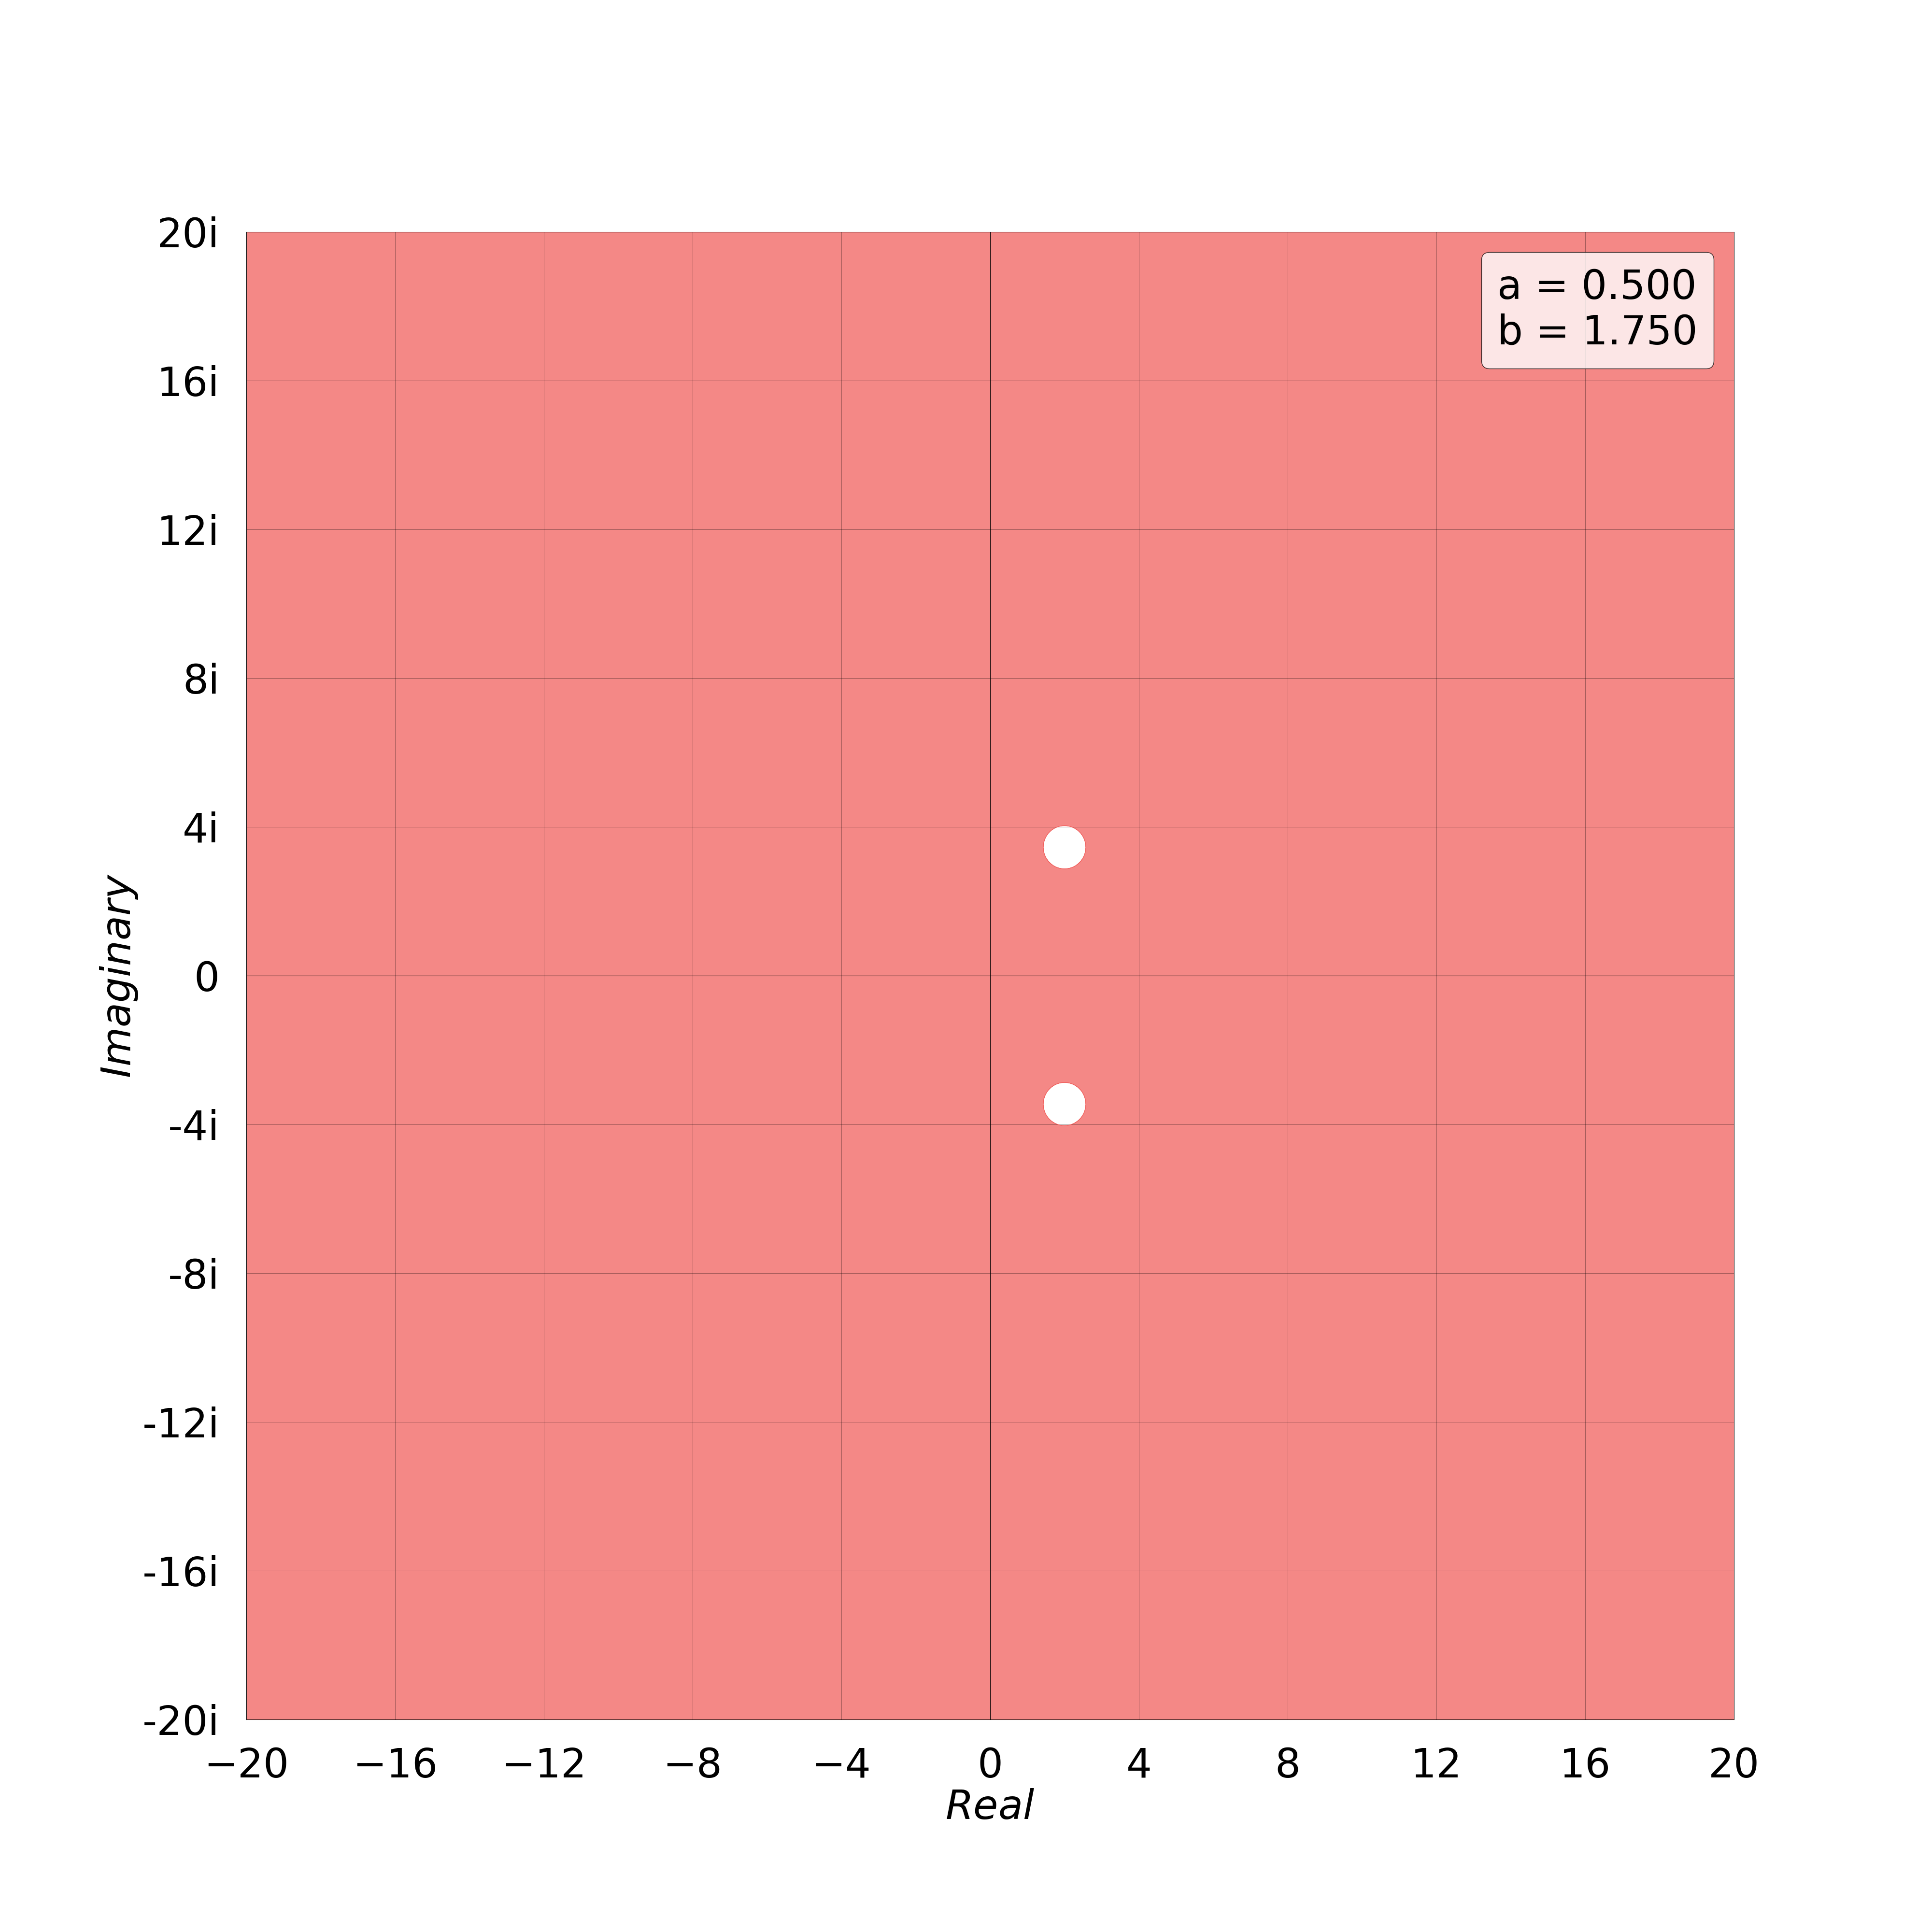
\includegraphics[width=0.32\textwidth]{Stability Regions/Videos/Varied b/Euler's Backward/a=0.5/frames/0350.png}
	\end{center}
	\columnbreak{}
	\begin{center}
		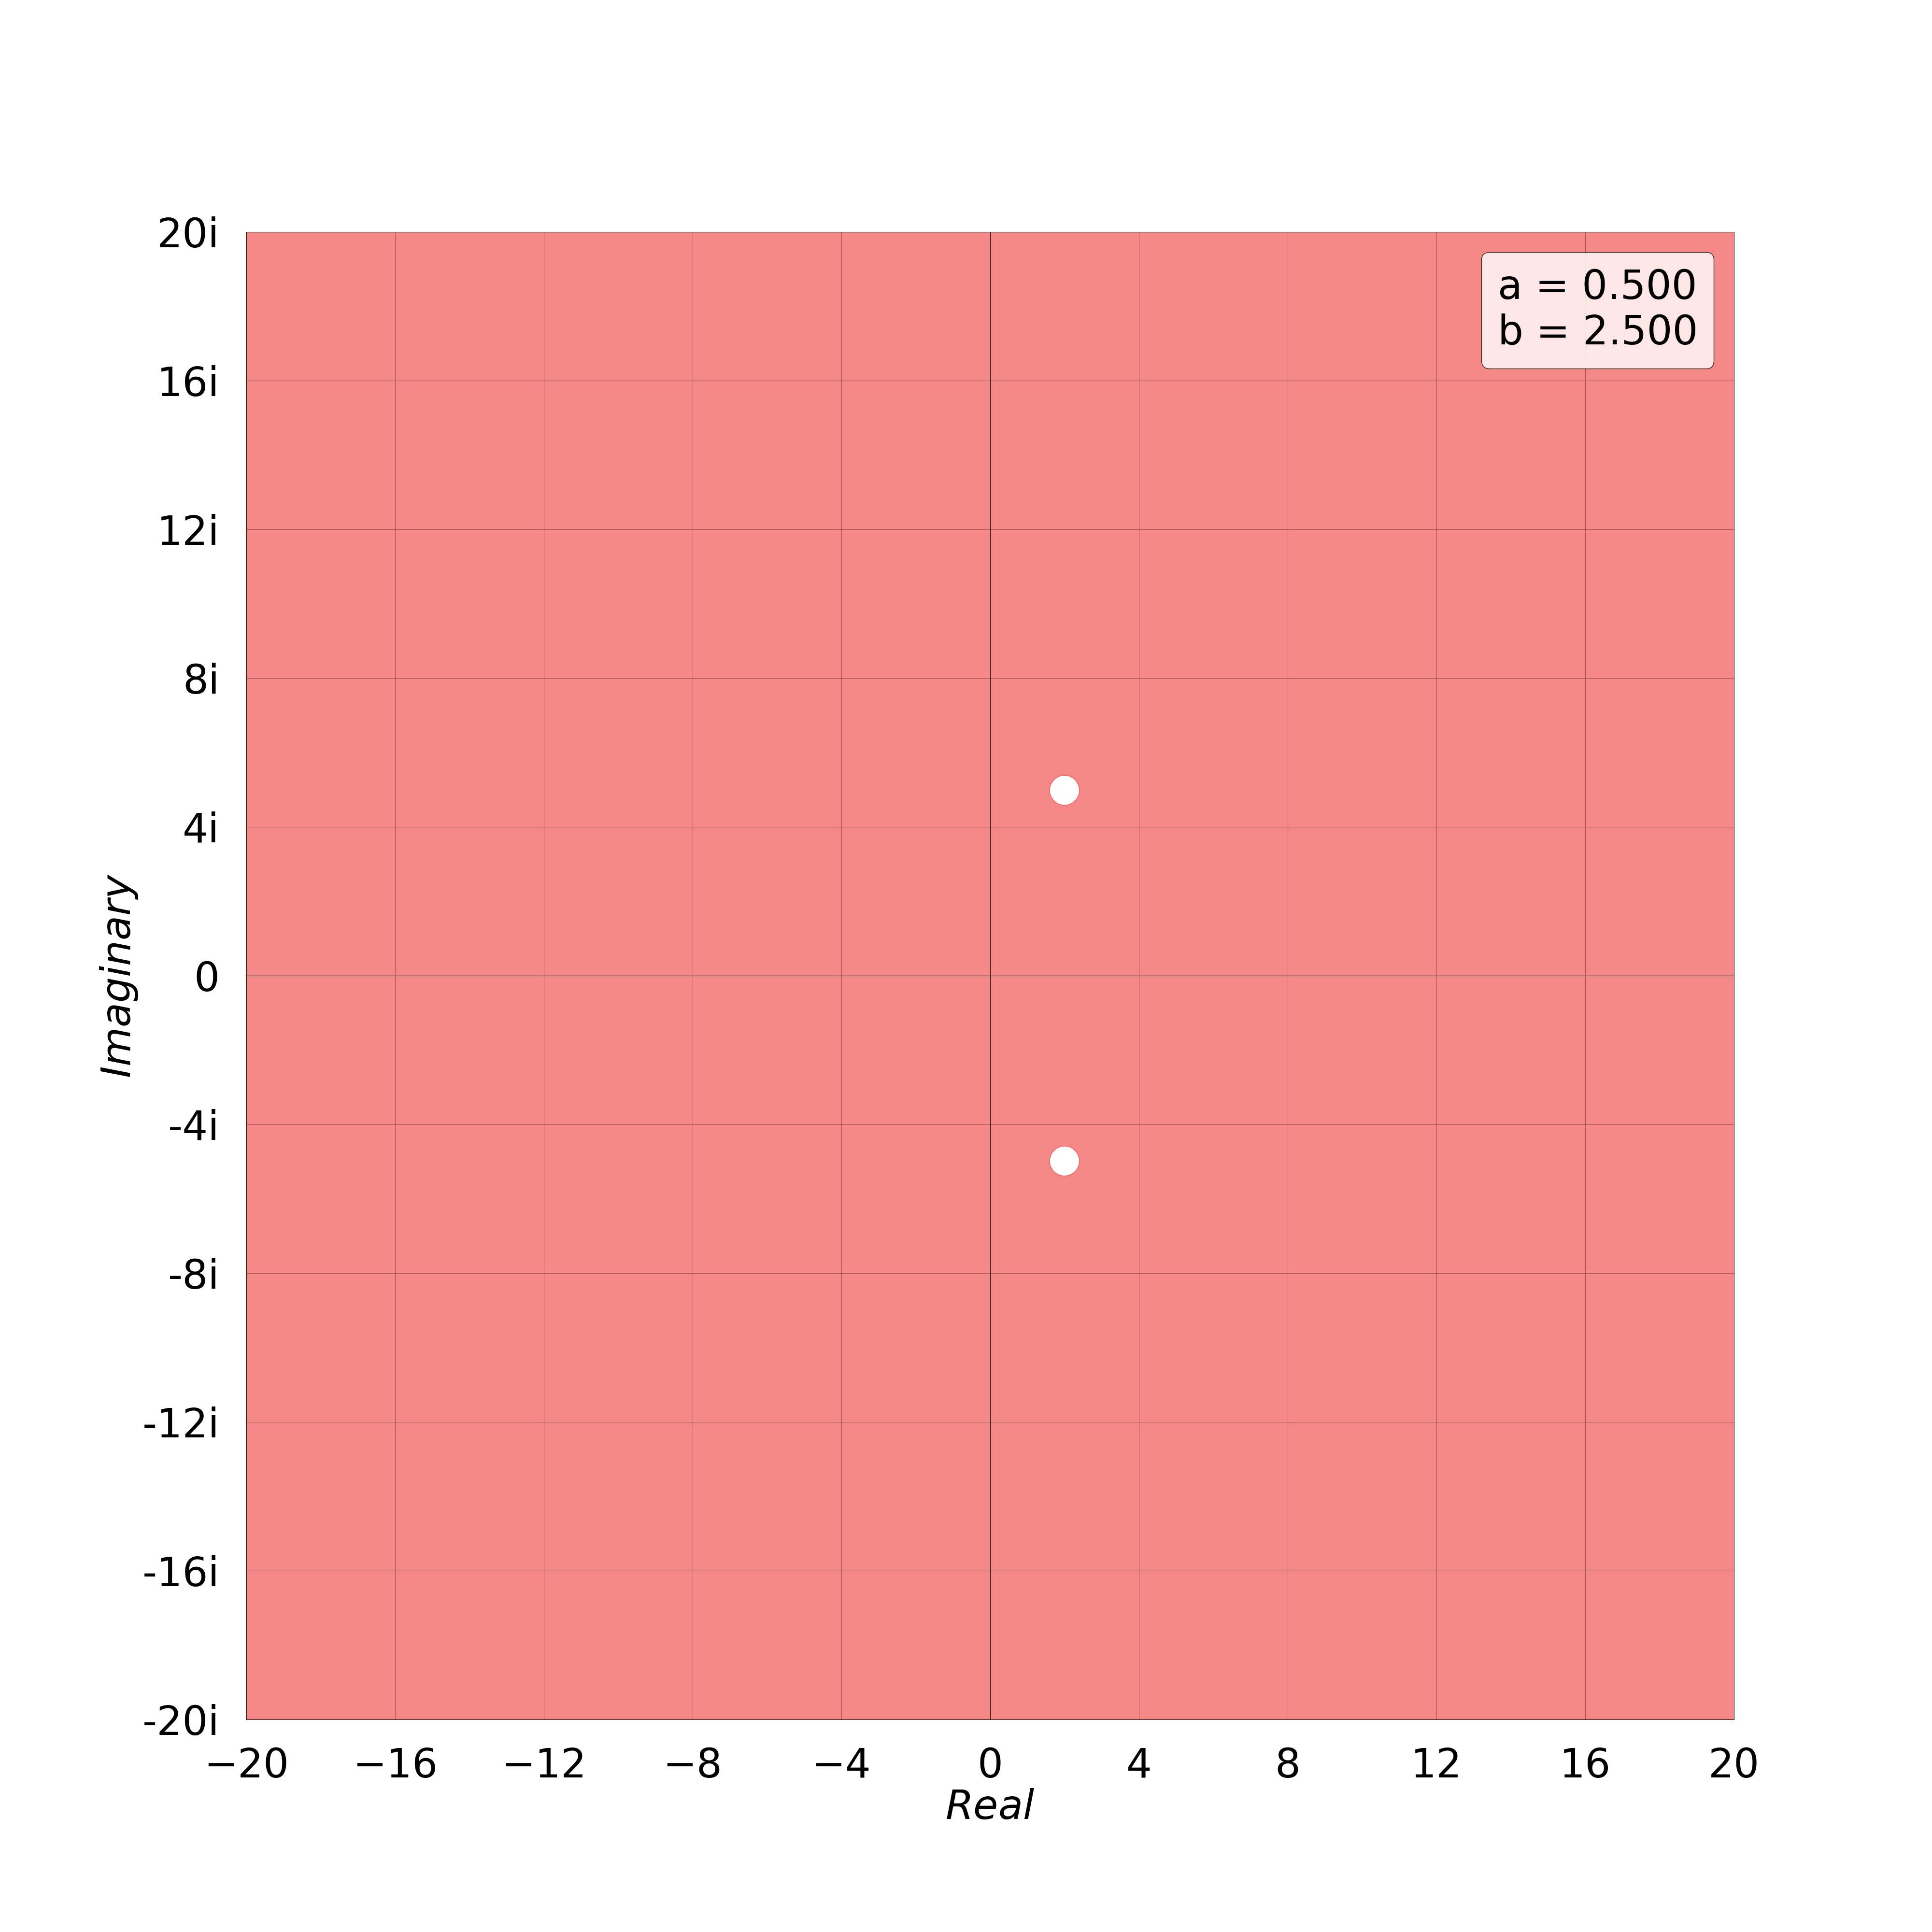
\includegraphics[width=0.32\textwidth]{Stability Regions/Videos/Varied b/Euler's Backward/a=0.5/frames/0500.png}
	\end{center}
\end{multicols}
\subsubsection{Runga-Kutta 4}
\vspace*{-0.65cm}
\begin{multicols}{3}
	\begin{center}
		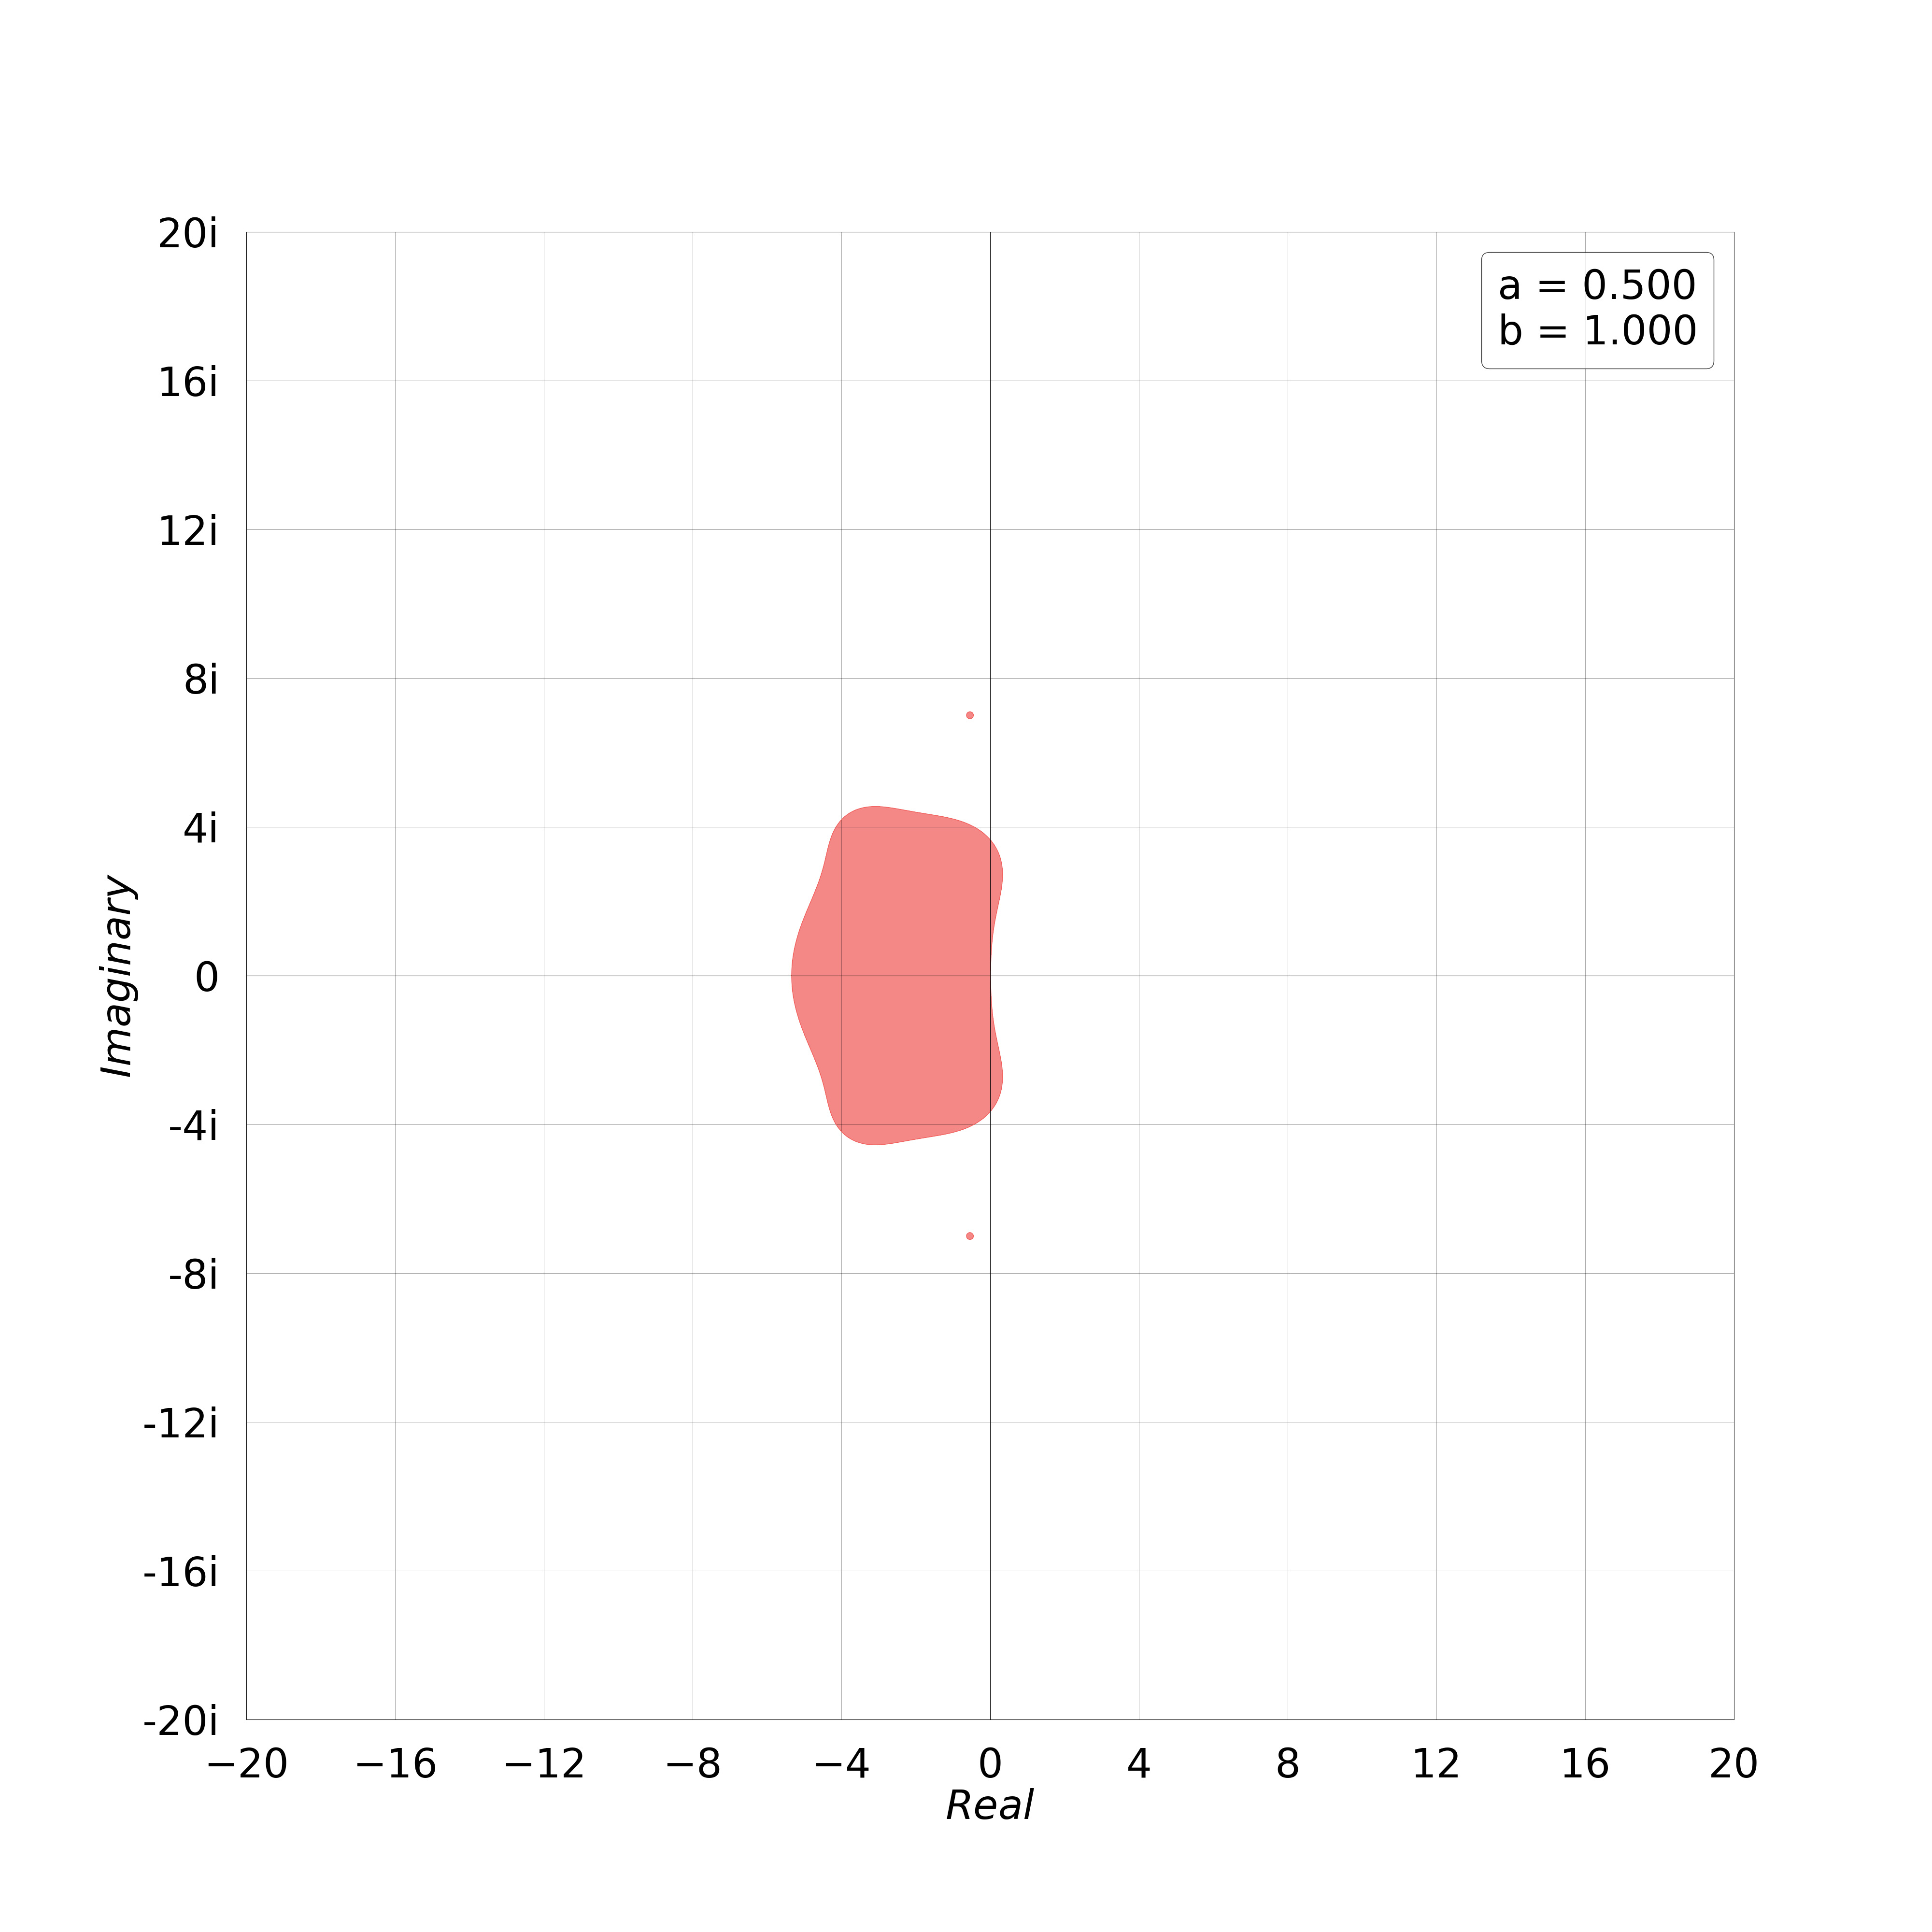
\includegraphics[width=0.32\textwidth]{Stability Regions/Videos/Varied b/Runge-Kutta 4/a=0.5/frames/0200.png}
	\end{center}
	\columnbreak{}
	\begin{center}
		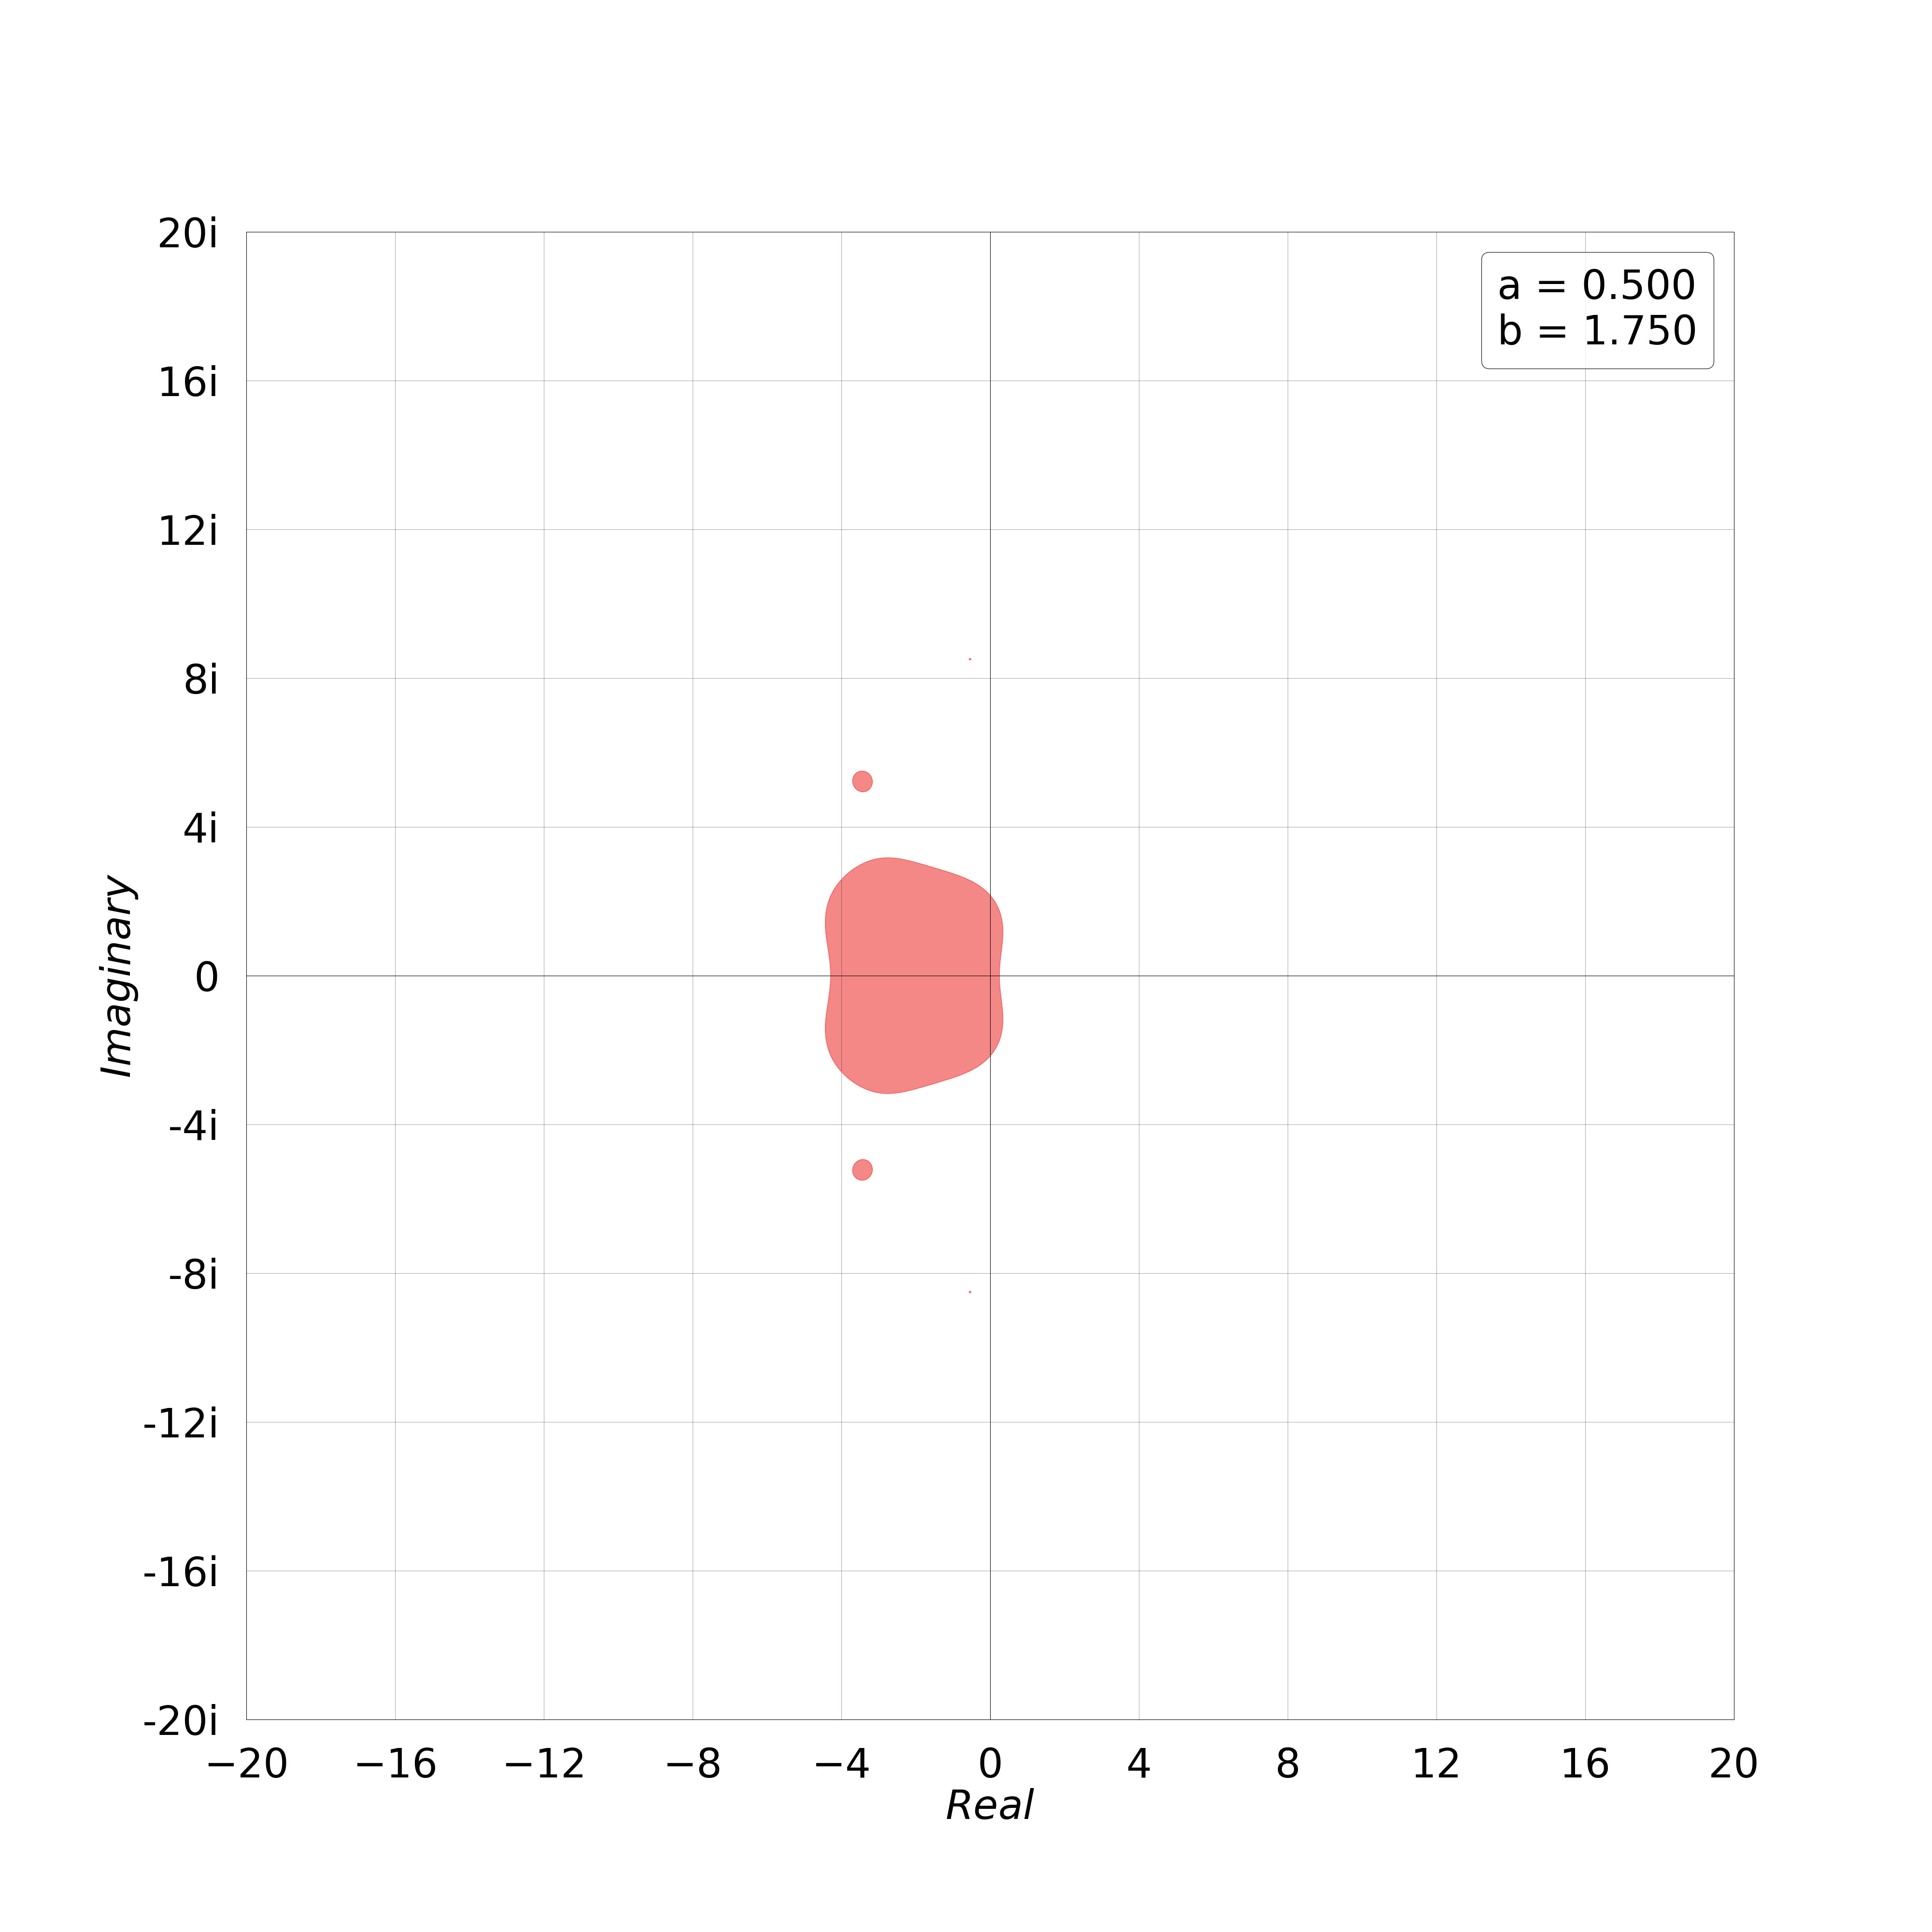
\includegraphics[width=0.32\textwidth]{Stability Regions/Videos/Varied b/Runge-Kutta 4/a=0.5/frames/0350.png}
	\end{center}
	\columnbreak{}
	\begin{center}
		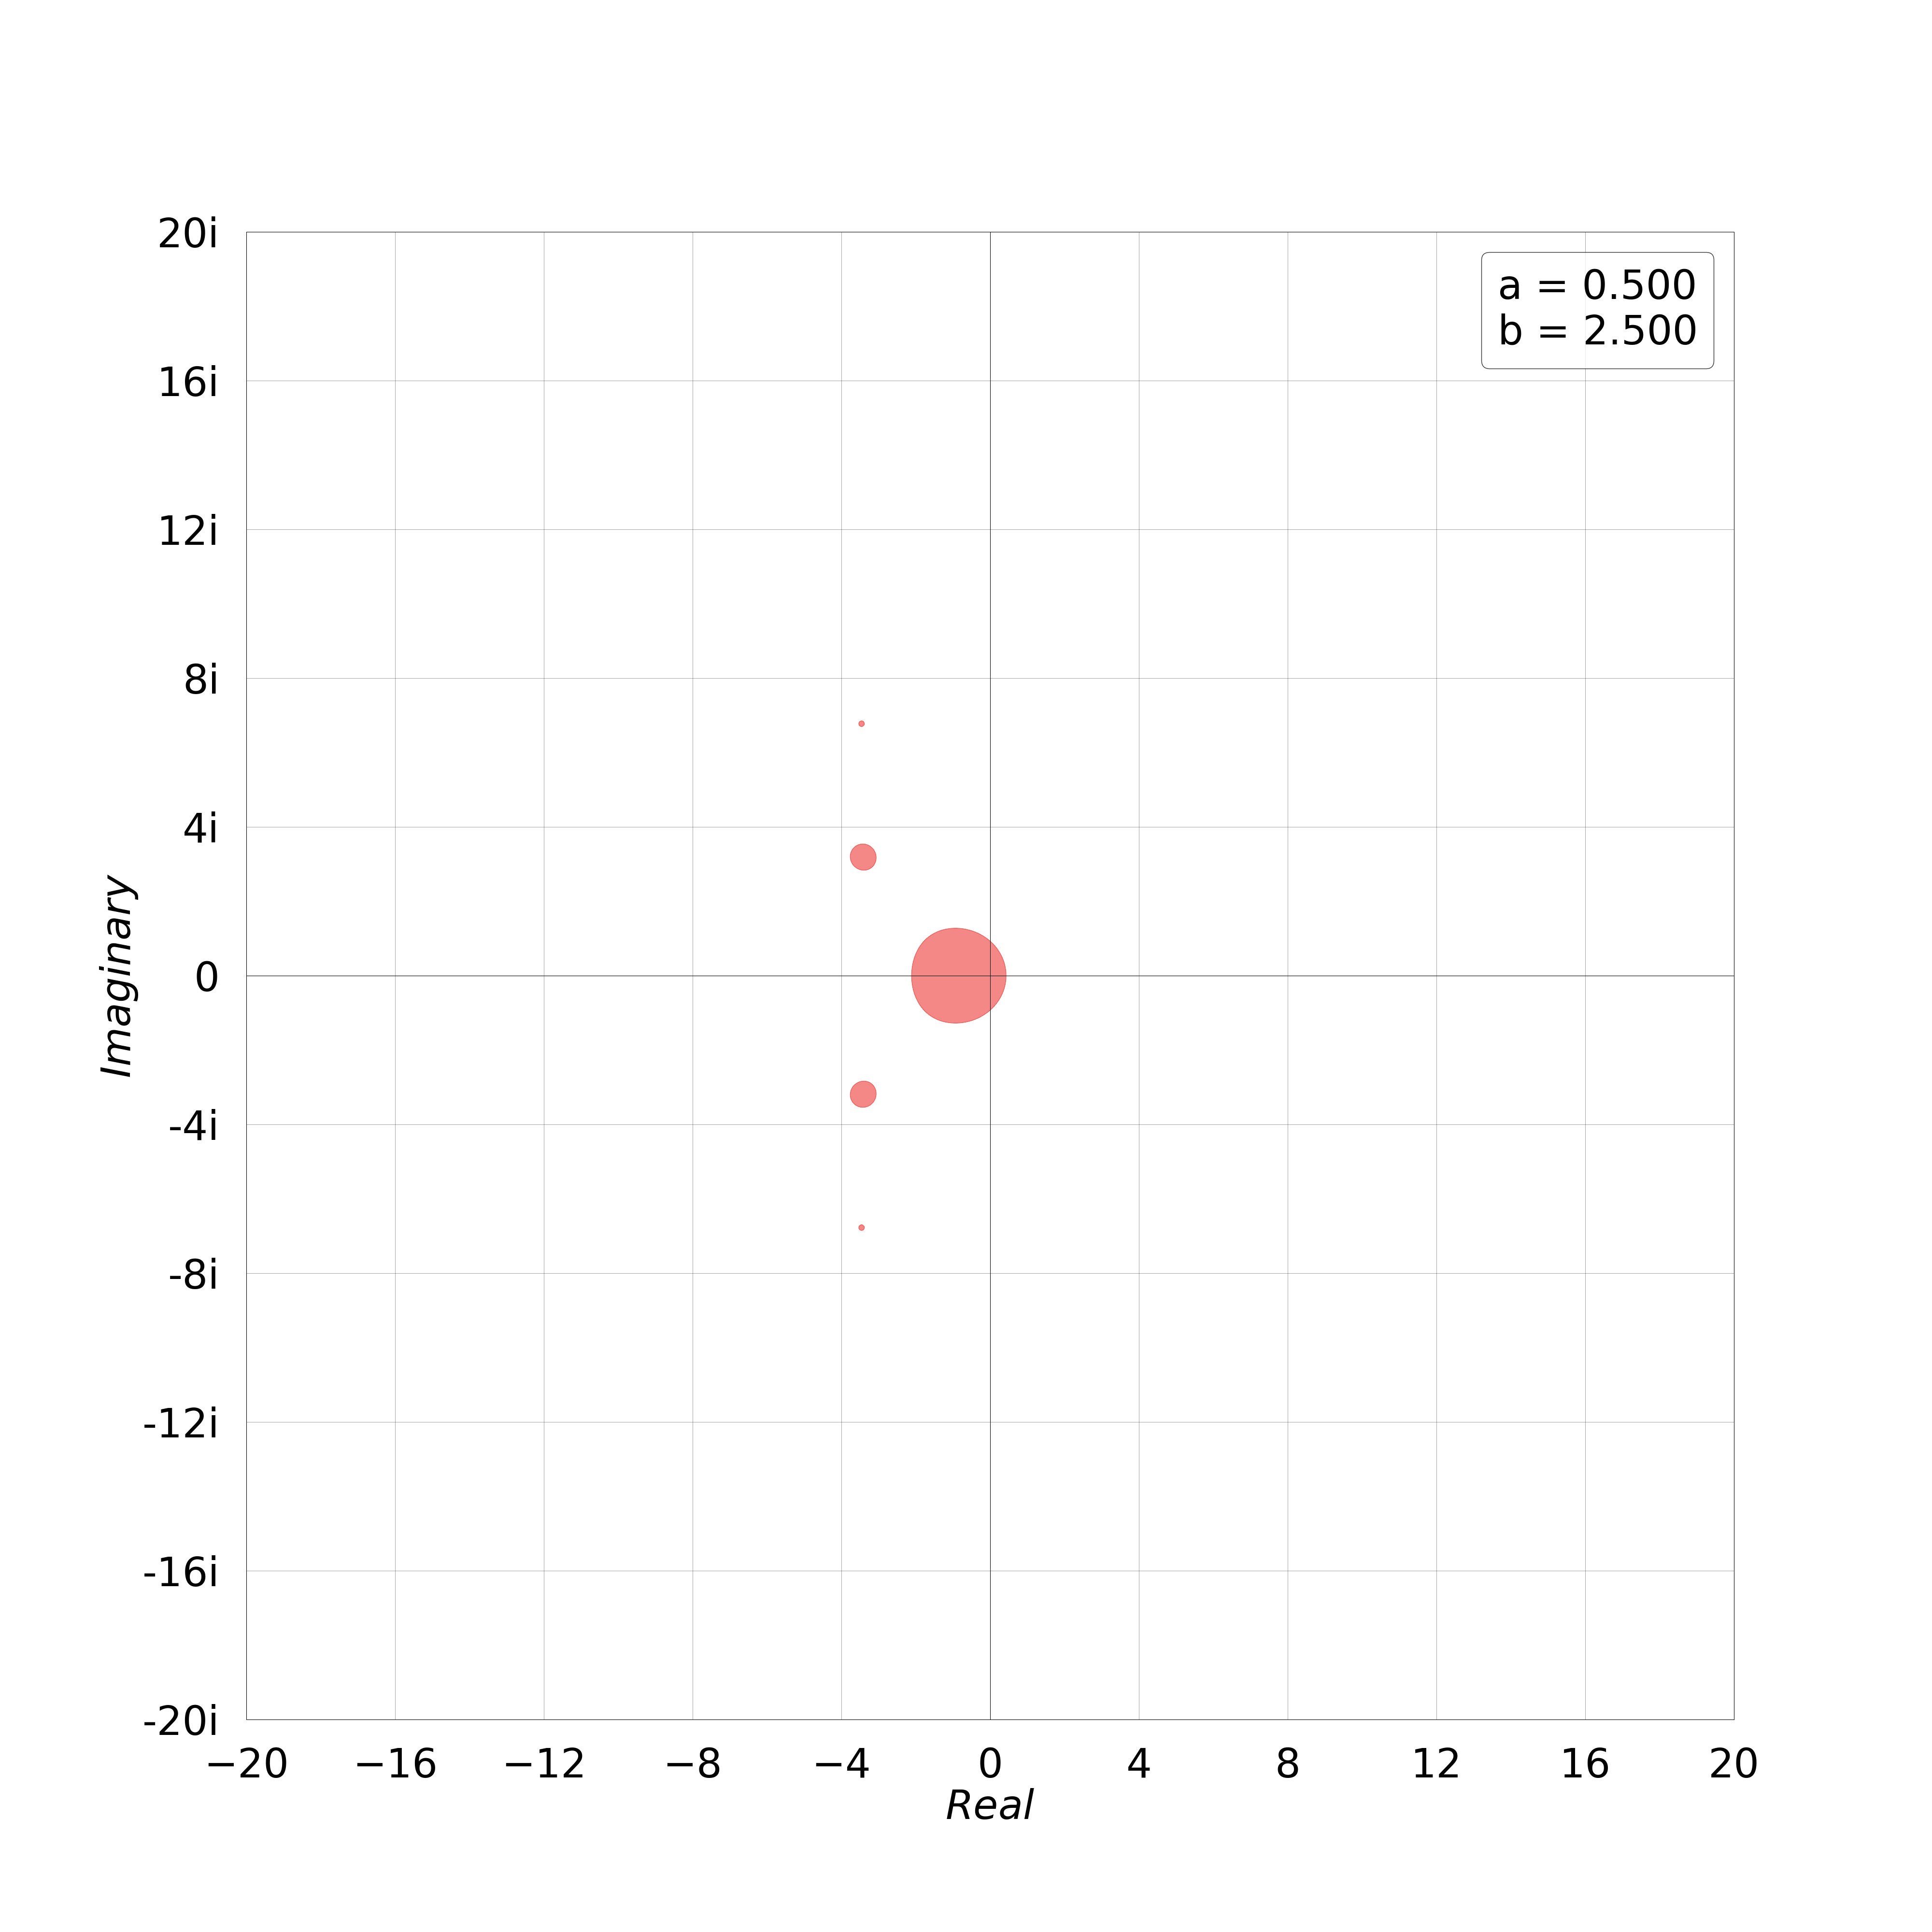
\includegraphics[width=0.32\textwidth]{Stability Regions/Videos/Varied b/Runge-Kutta 4/a=0.5/frames/0500.png}
	\end{center}
\end{multicols}
\newpage
\subsection{Varying a}
\par We can also vary $a$ and see how the stability regions change.\\
This falls outside the scope of complex conjugate step pairs.\\
Consequently, these stability regions can only be interpreted for $\lambda \in \bC\setminus\bR$ (If you believe Conjecture 1).\\
In the cases below, we have set $b = \frac{\lh}{2}$\\
Videos showing the stability regions for varying $a$ values can be found in the \textit{GitHub Repository}\cite{GitHub_Repo} for this project.\\
The same process was followed as in the previous section:\\
The videos were created frame-by-frame using the script in Appendix~\ref{appendix:video_frames}.\\
The frames were stiched together using the script in Appendix~\ref{appendix:frames_to_video}.\\
Below are some of the video frames for each method.\\
\textbf{Observations:}
\begin{itemize}
	\item[$\cdot$] The stability region for varying $a$ values is not symmetric across the real axis, except for the case where $a = 0.5$.
	\item[$\cdot$] The stability regions for $a = 0.5 \pm \alpha$ are symmetric to each other across the real axis for any $|\alpha| < 0.5$.
	\item[$\cdot$] The stability region for Euler's Backward Method is the complement of that for Euler's Forward Method, after it has been reflected across the imaginary axis.
\end{itemize}
\subsubsection{Euler's Forward}
\vspace*{-0.65cm}
\begin{multicols}{3}
	\begin{center}
		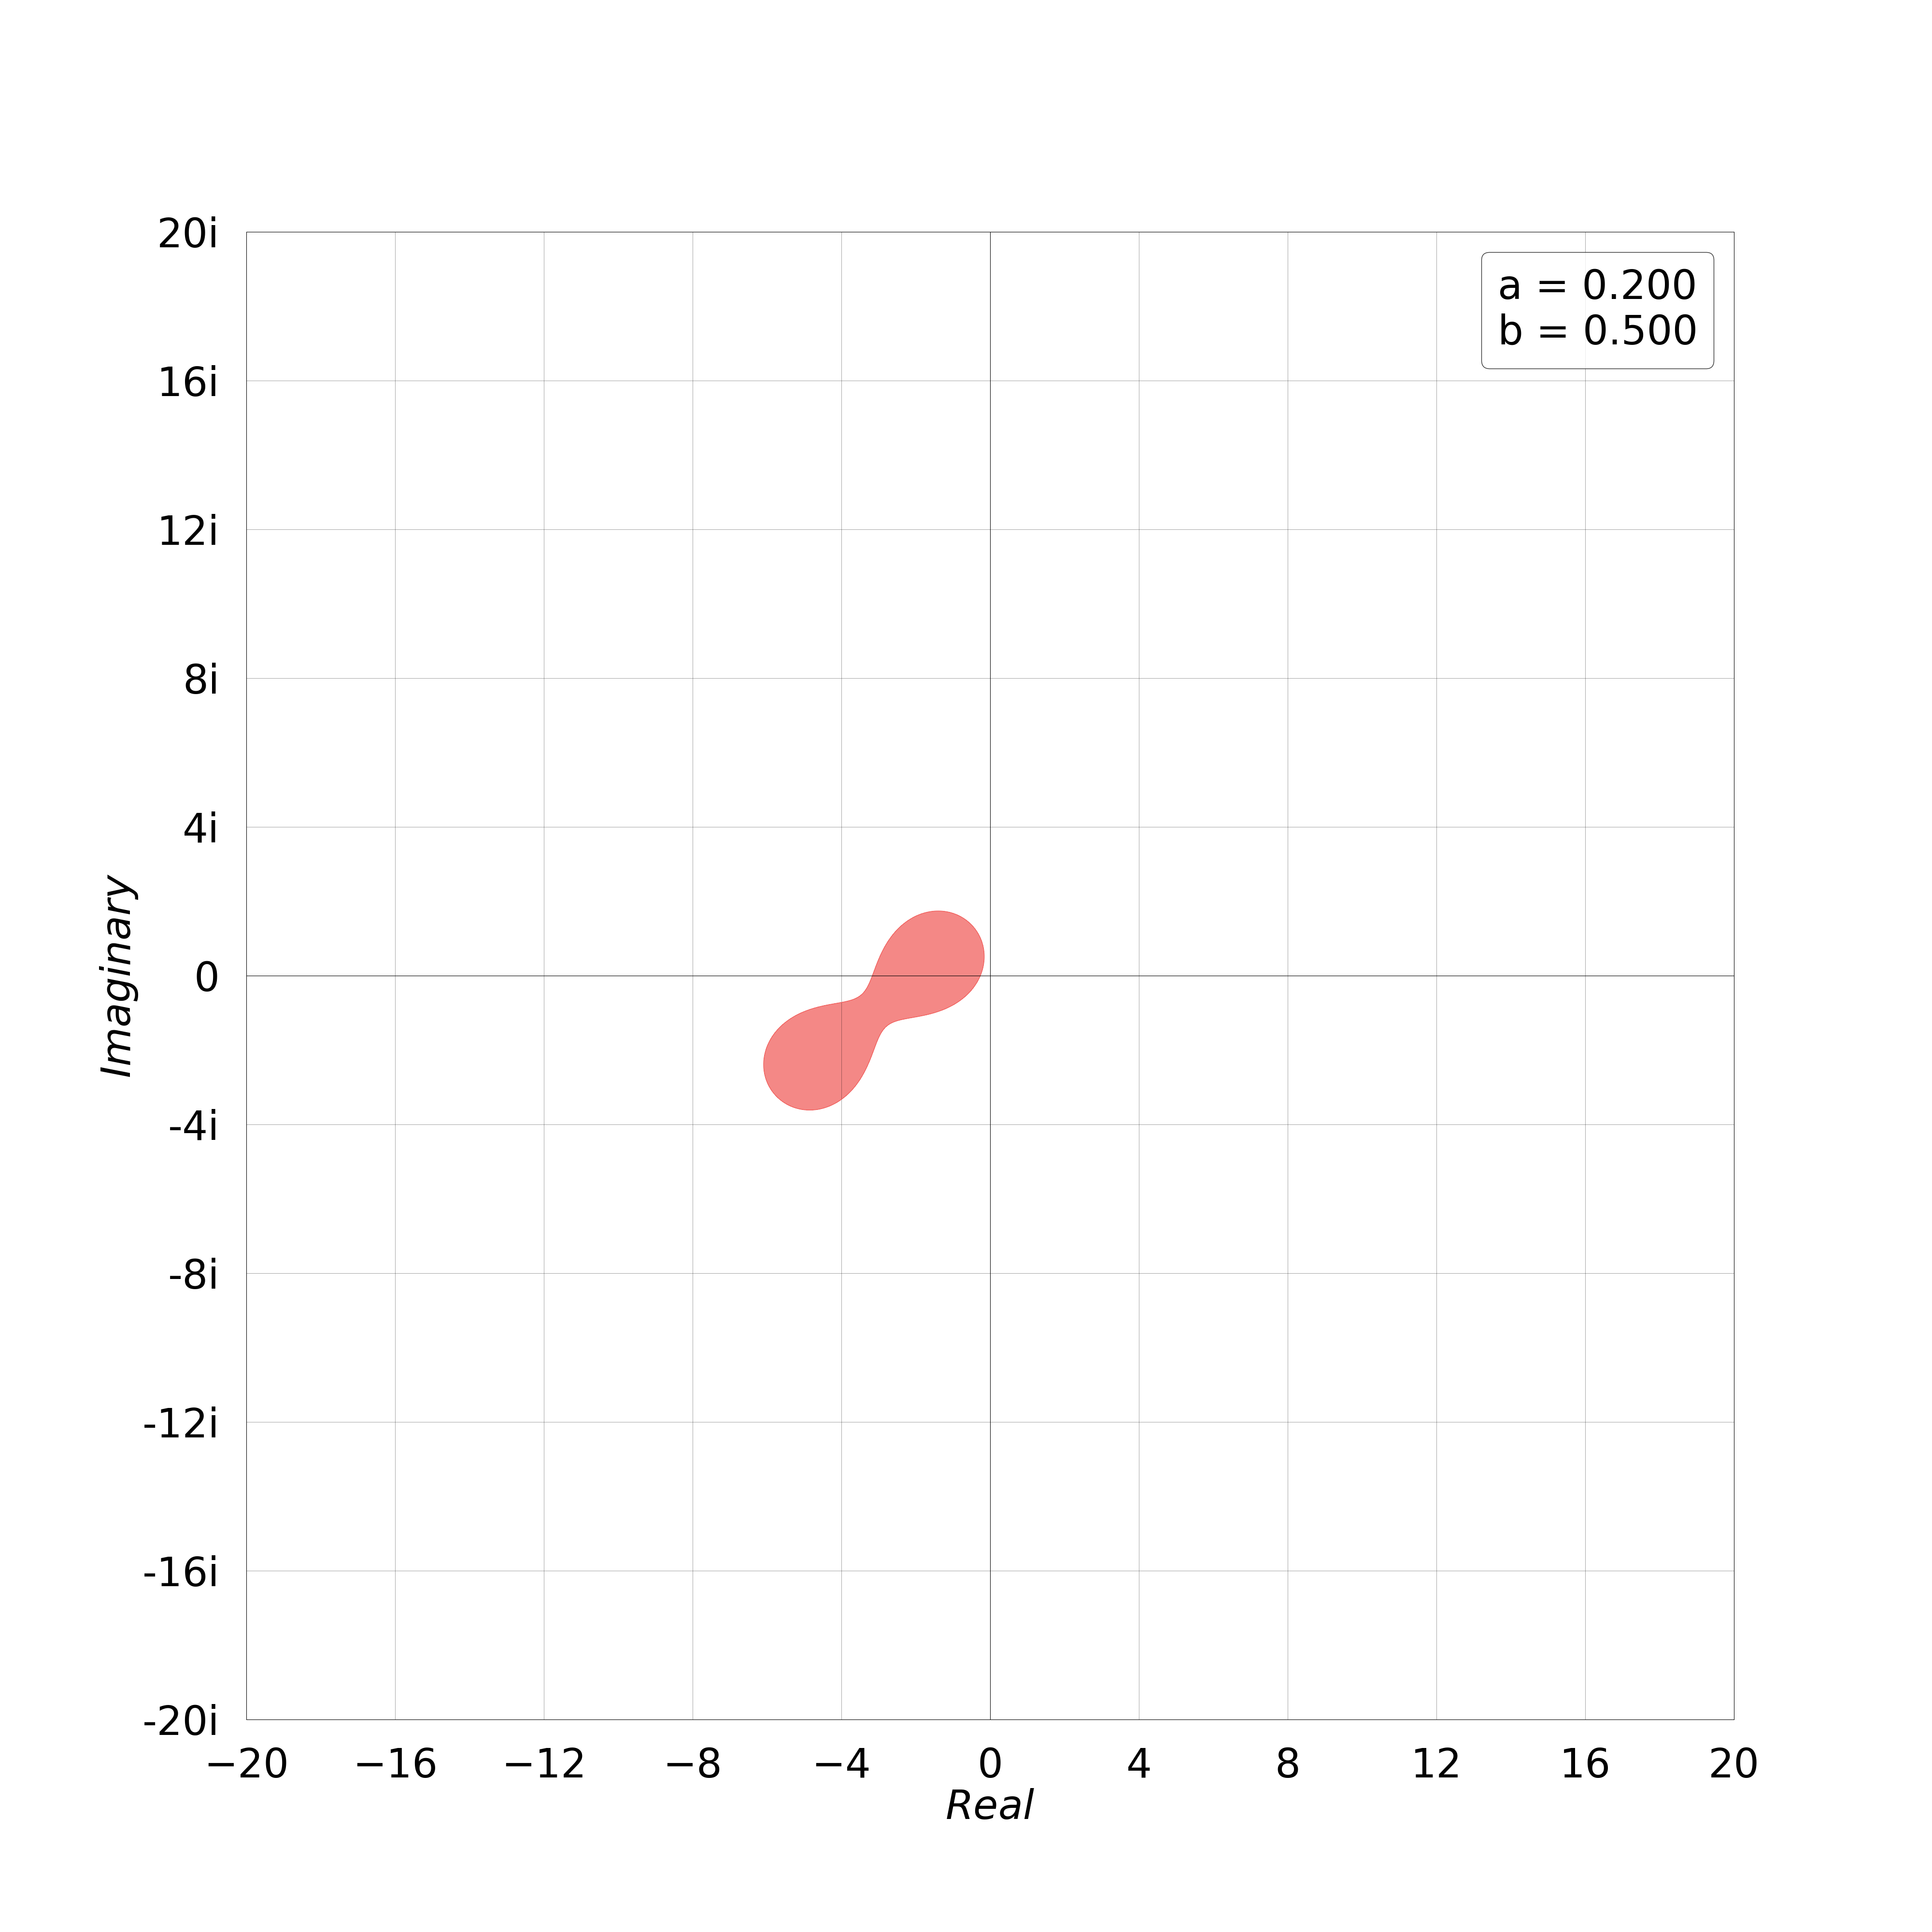
\includegraphics[width=0.32\textwidth]{Stability Regions/Videos/Varied a/Euler's Forward/b=0.5/frames/0200.png}
	\end{center}
	\columnbreak{}
	\begin{center}
		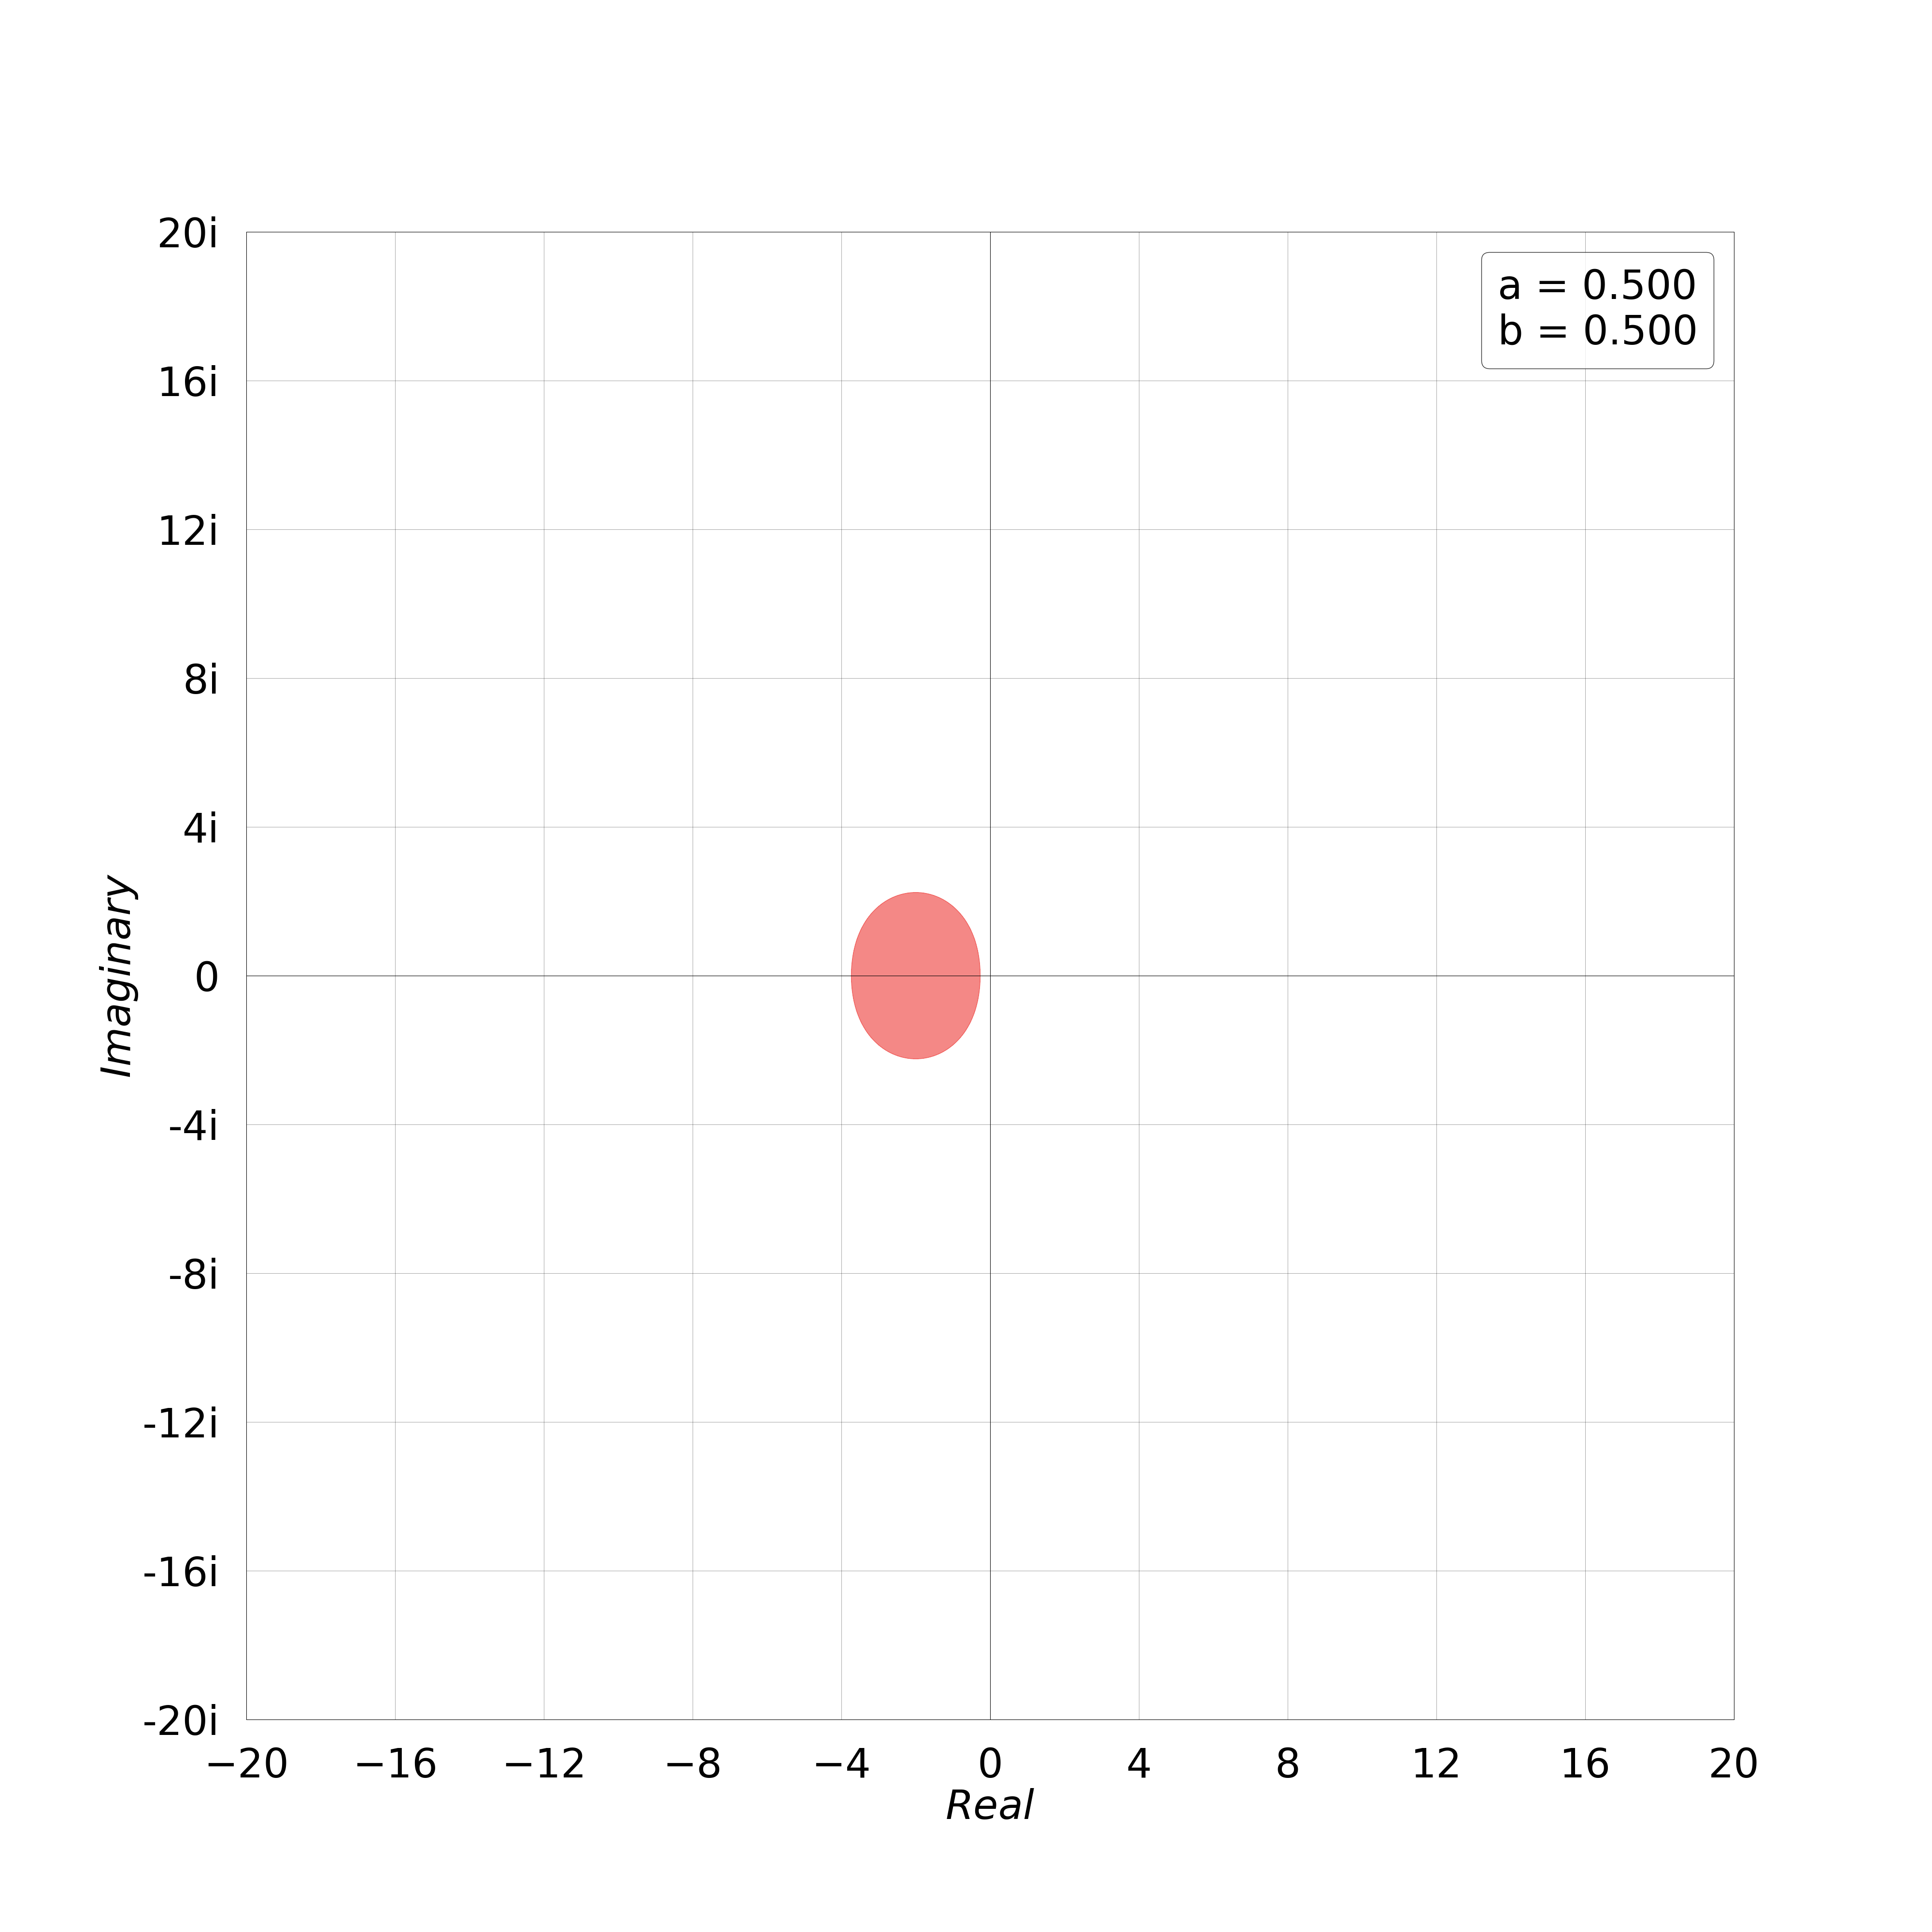
\includegraphics[width=0.32\textwidth]{Stability Regions/Videos/Varied a/Euler's Forward/b=0.5/frames/0500.png}
	\end{center}
	\columnbreak{}
	\begin{center}
		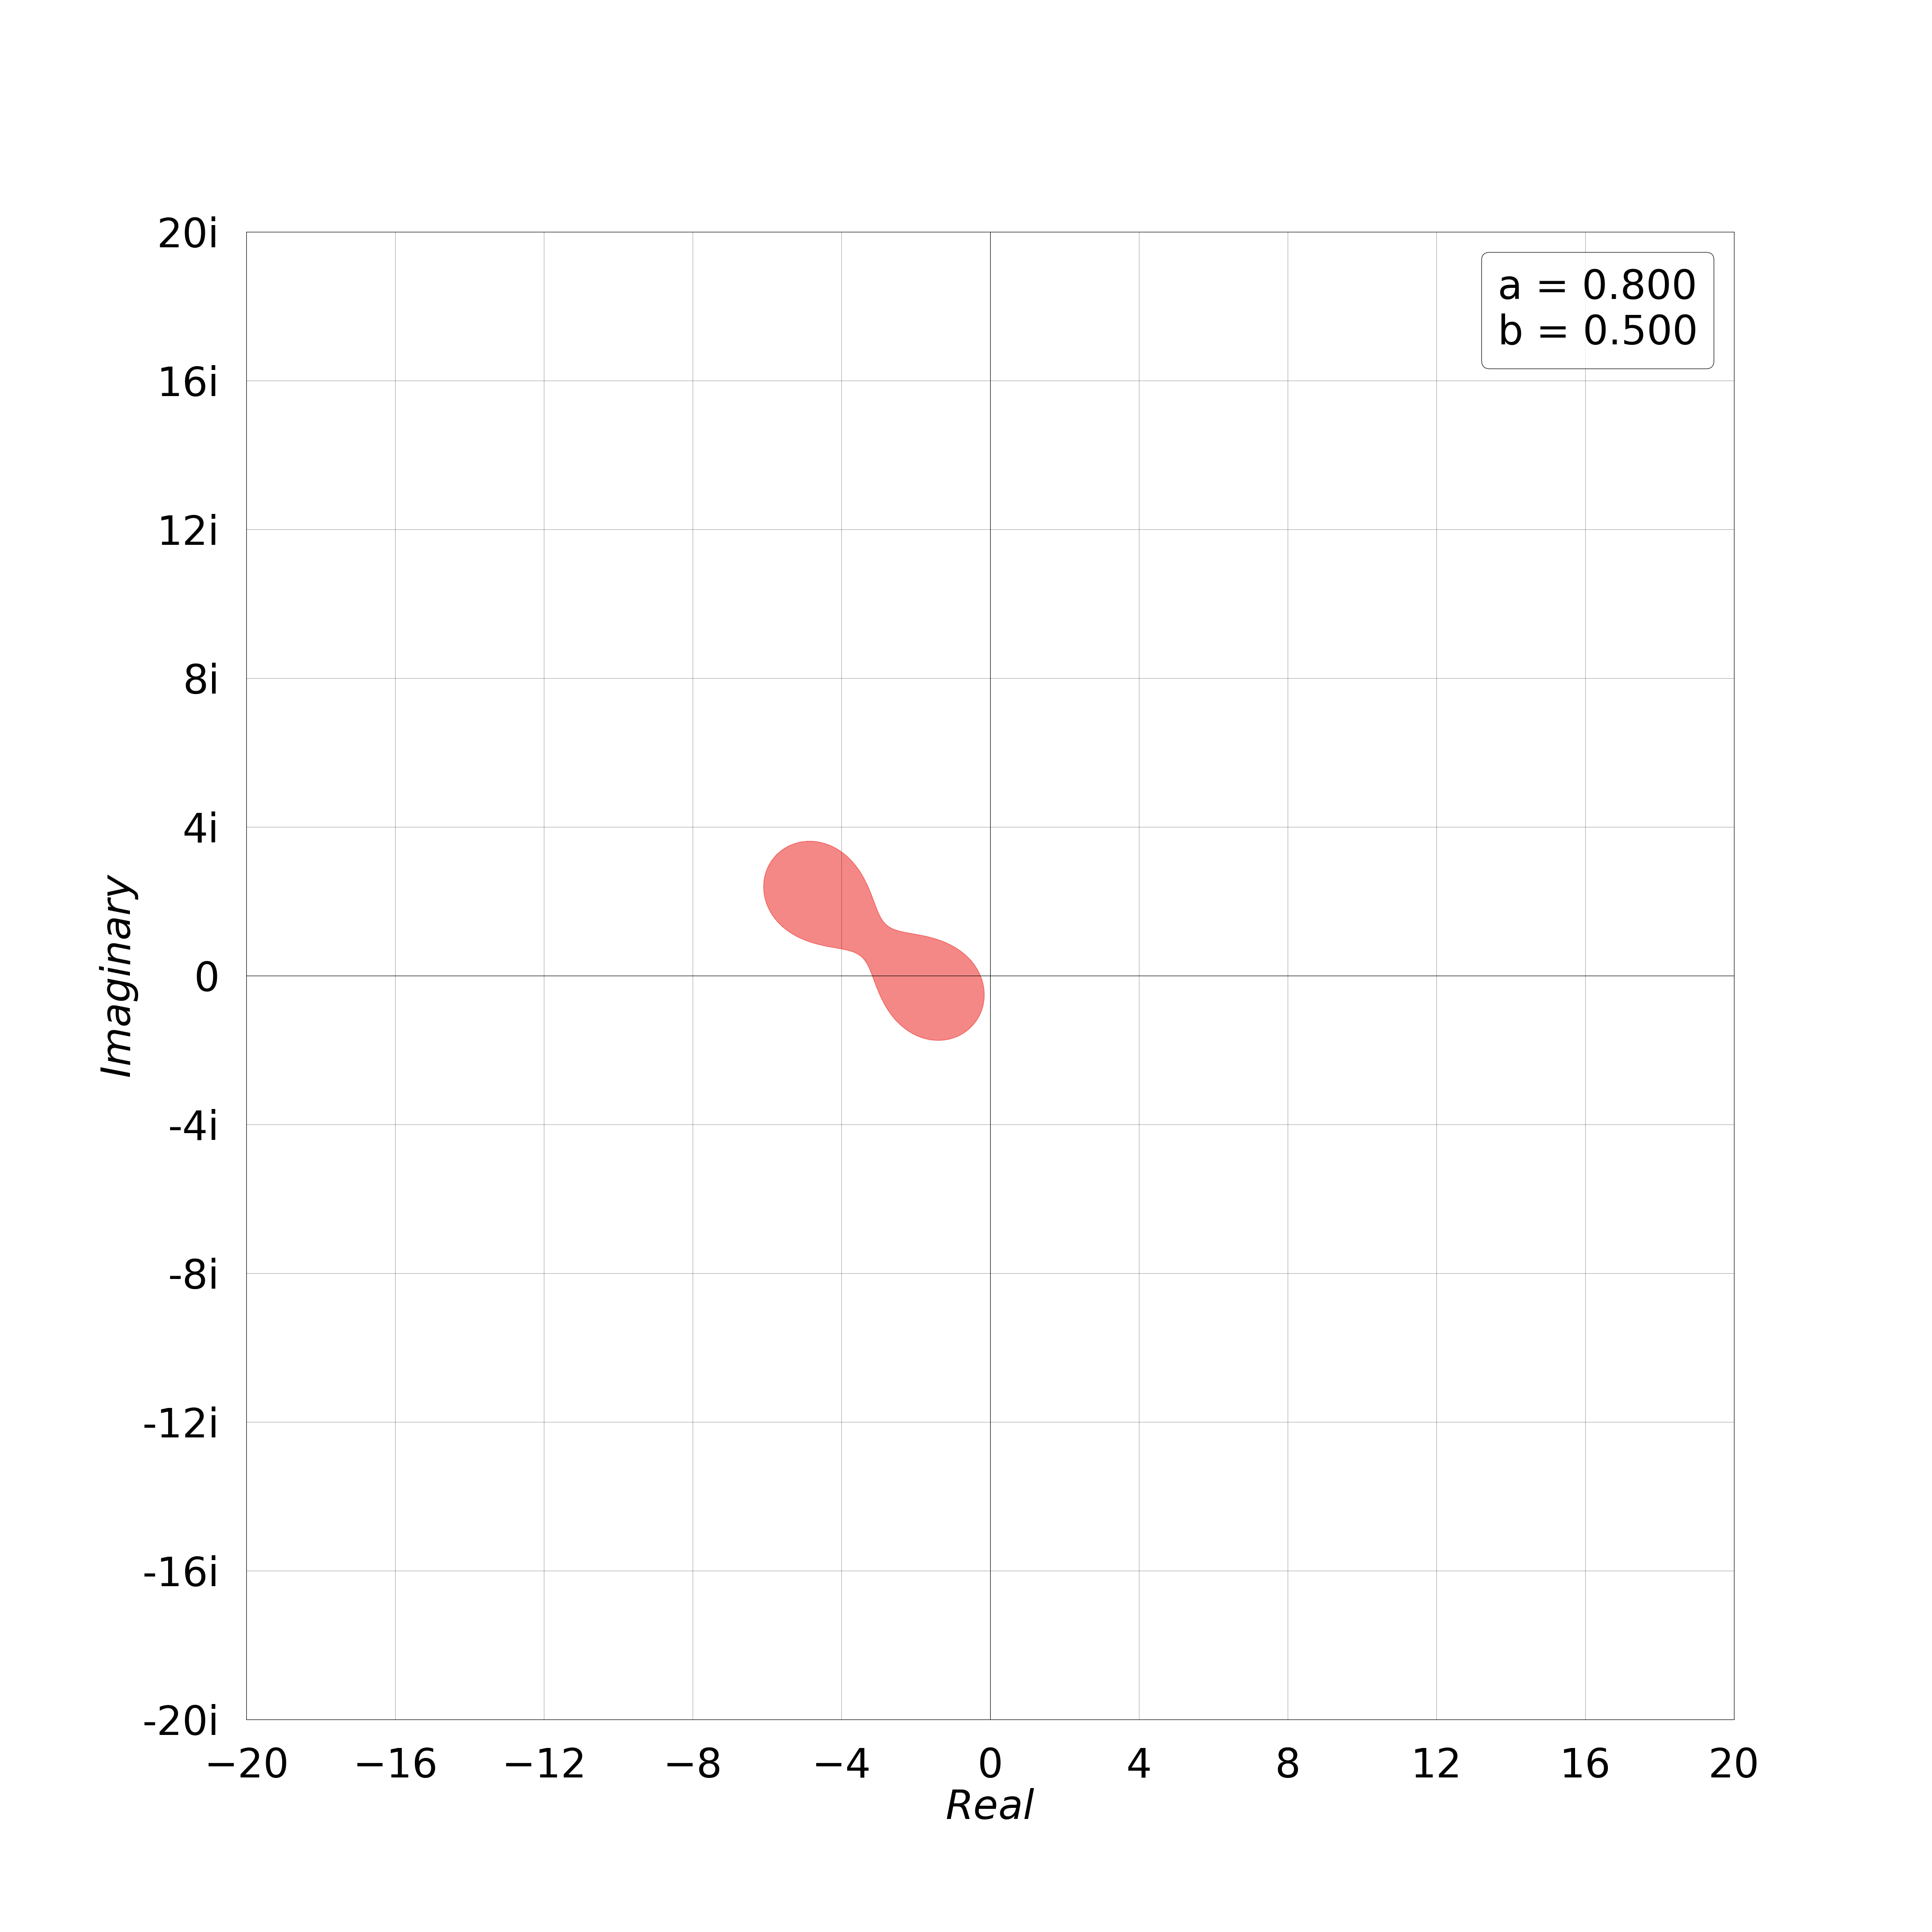
\includegraphics[width=0.32\textwidth]{Stability Regions/Videos/Varied a/Euler's Forward/b=0.5/frames/0800.png}
	\end{center}
\end{multicols}
\subsubsection{Euler's Backward}
\vspace*{-0.65cm}
\begin{multicols}{3}
	\begin{center}
		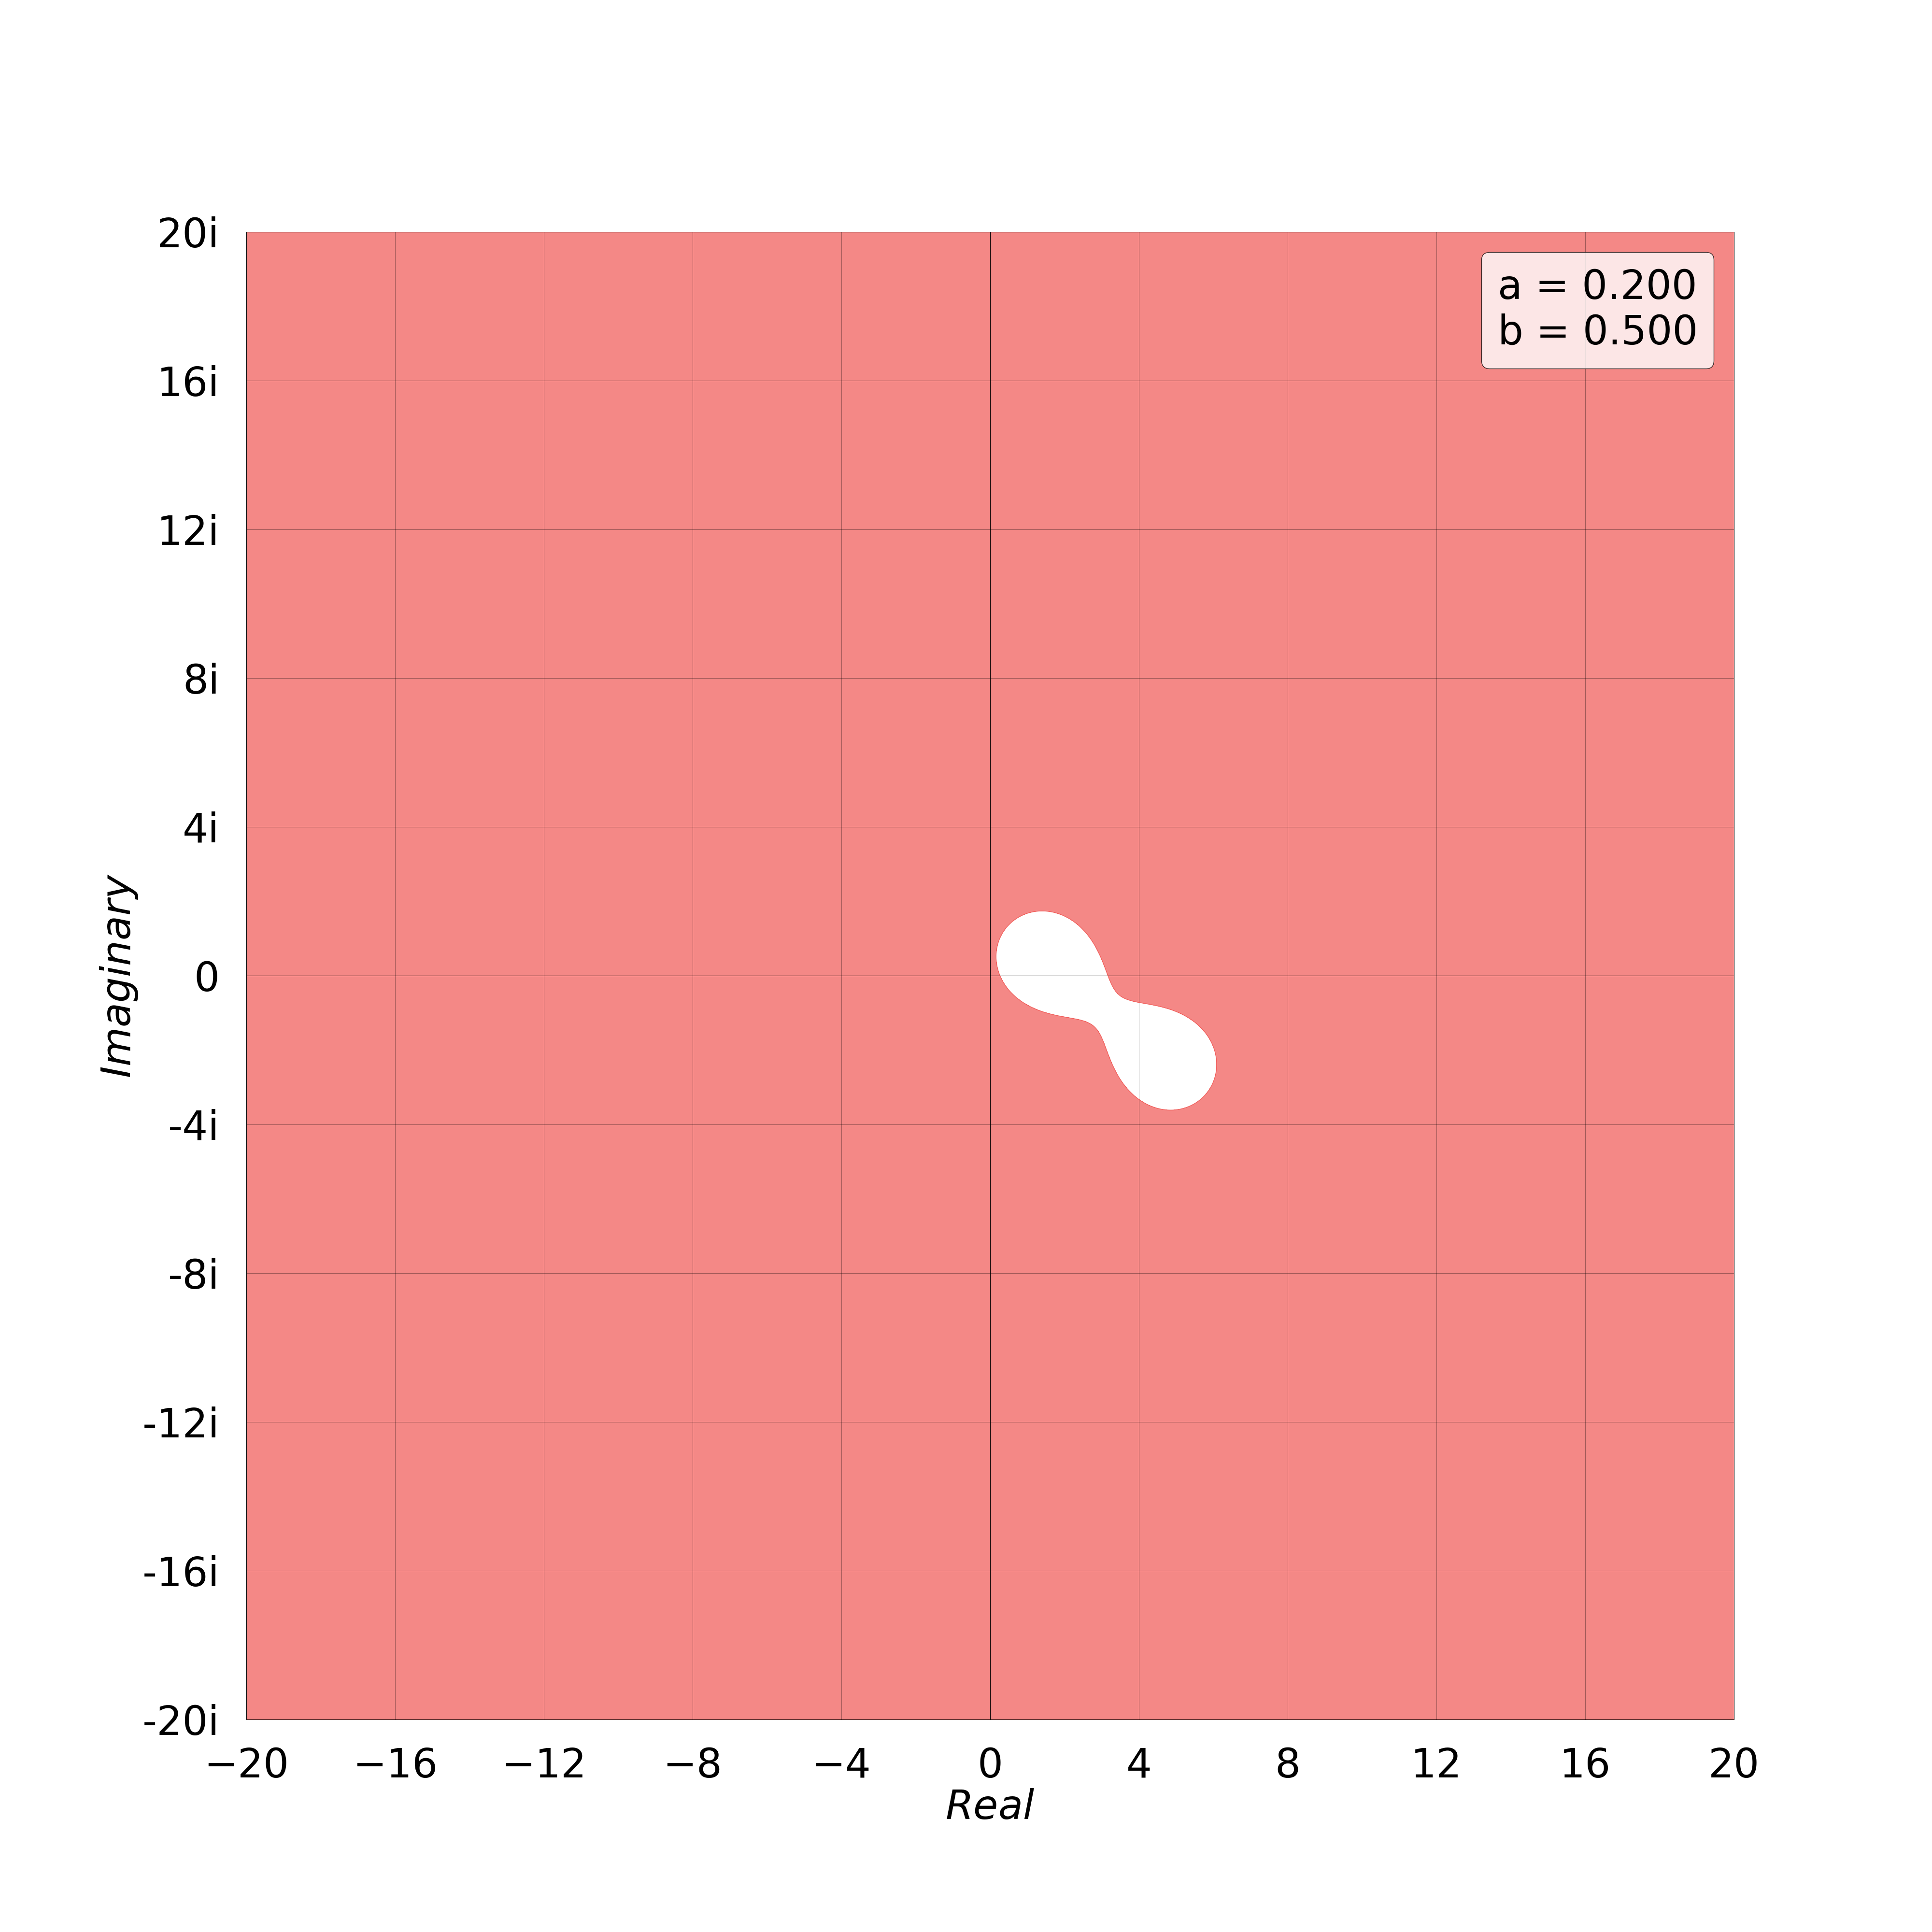
\includegraphics[width=0.32\textwidth]{Stability Regions/Videos/Varied a/Euler's Backward/b=0.5/frames/0200.png}
	\end{center}
	\columnbreak{}
	\begin{center}
		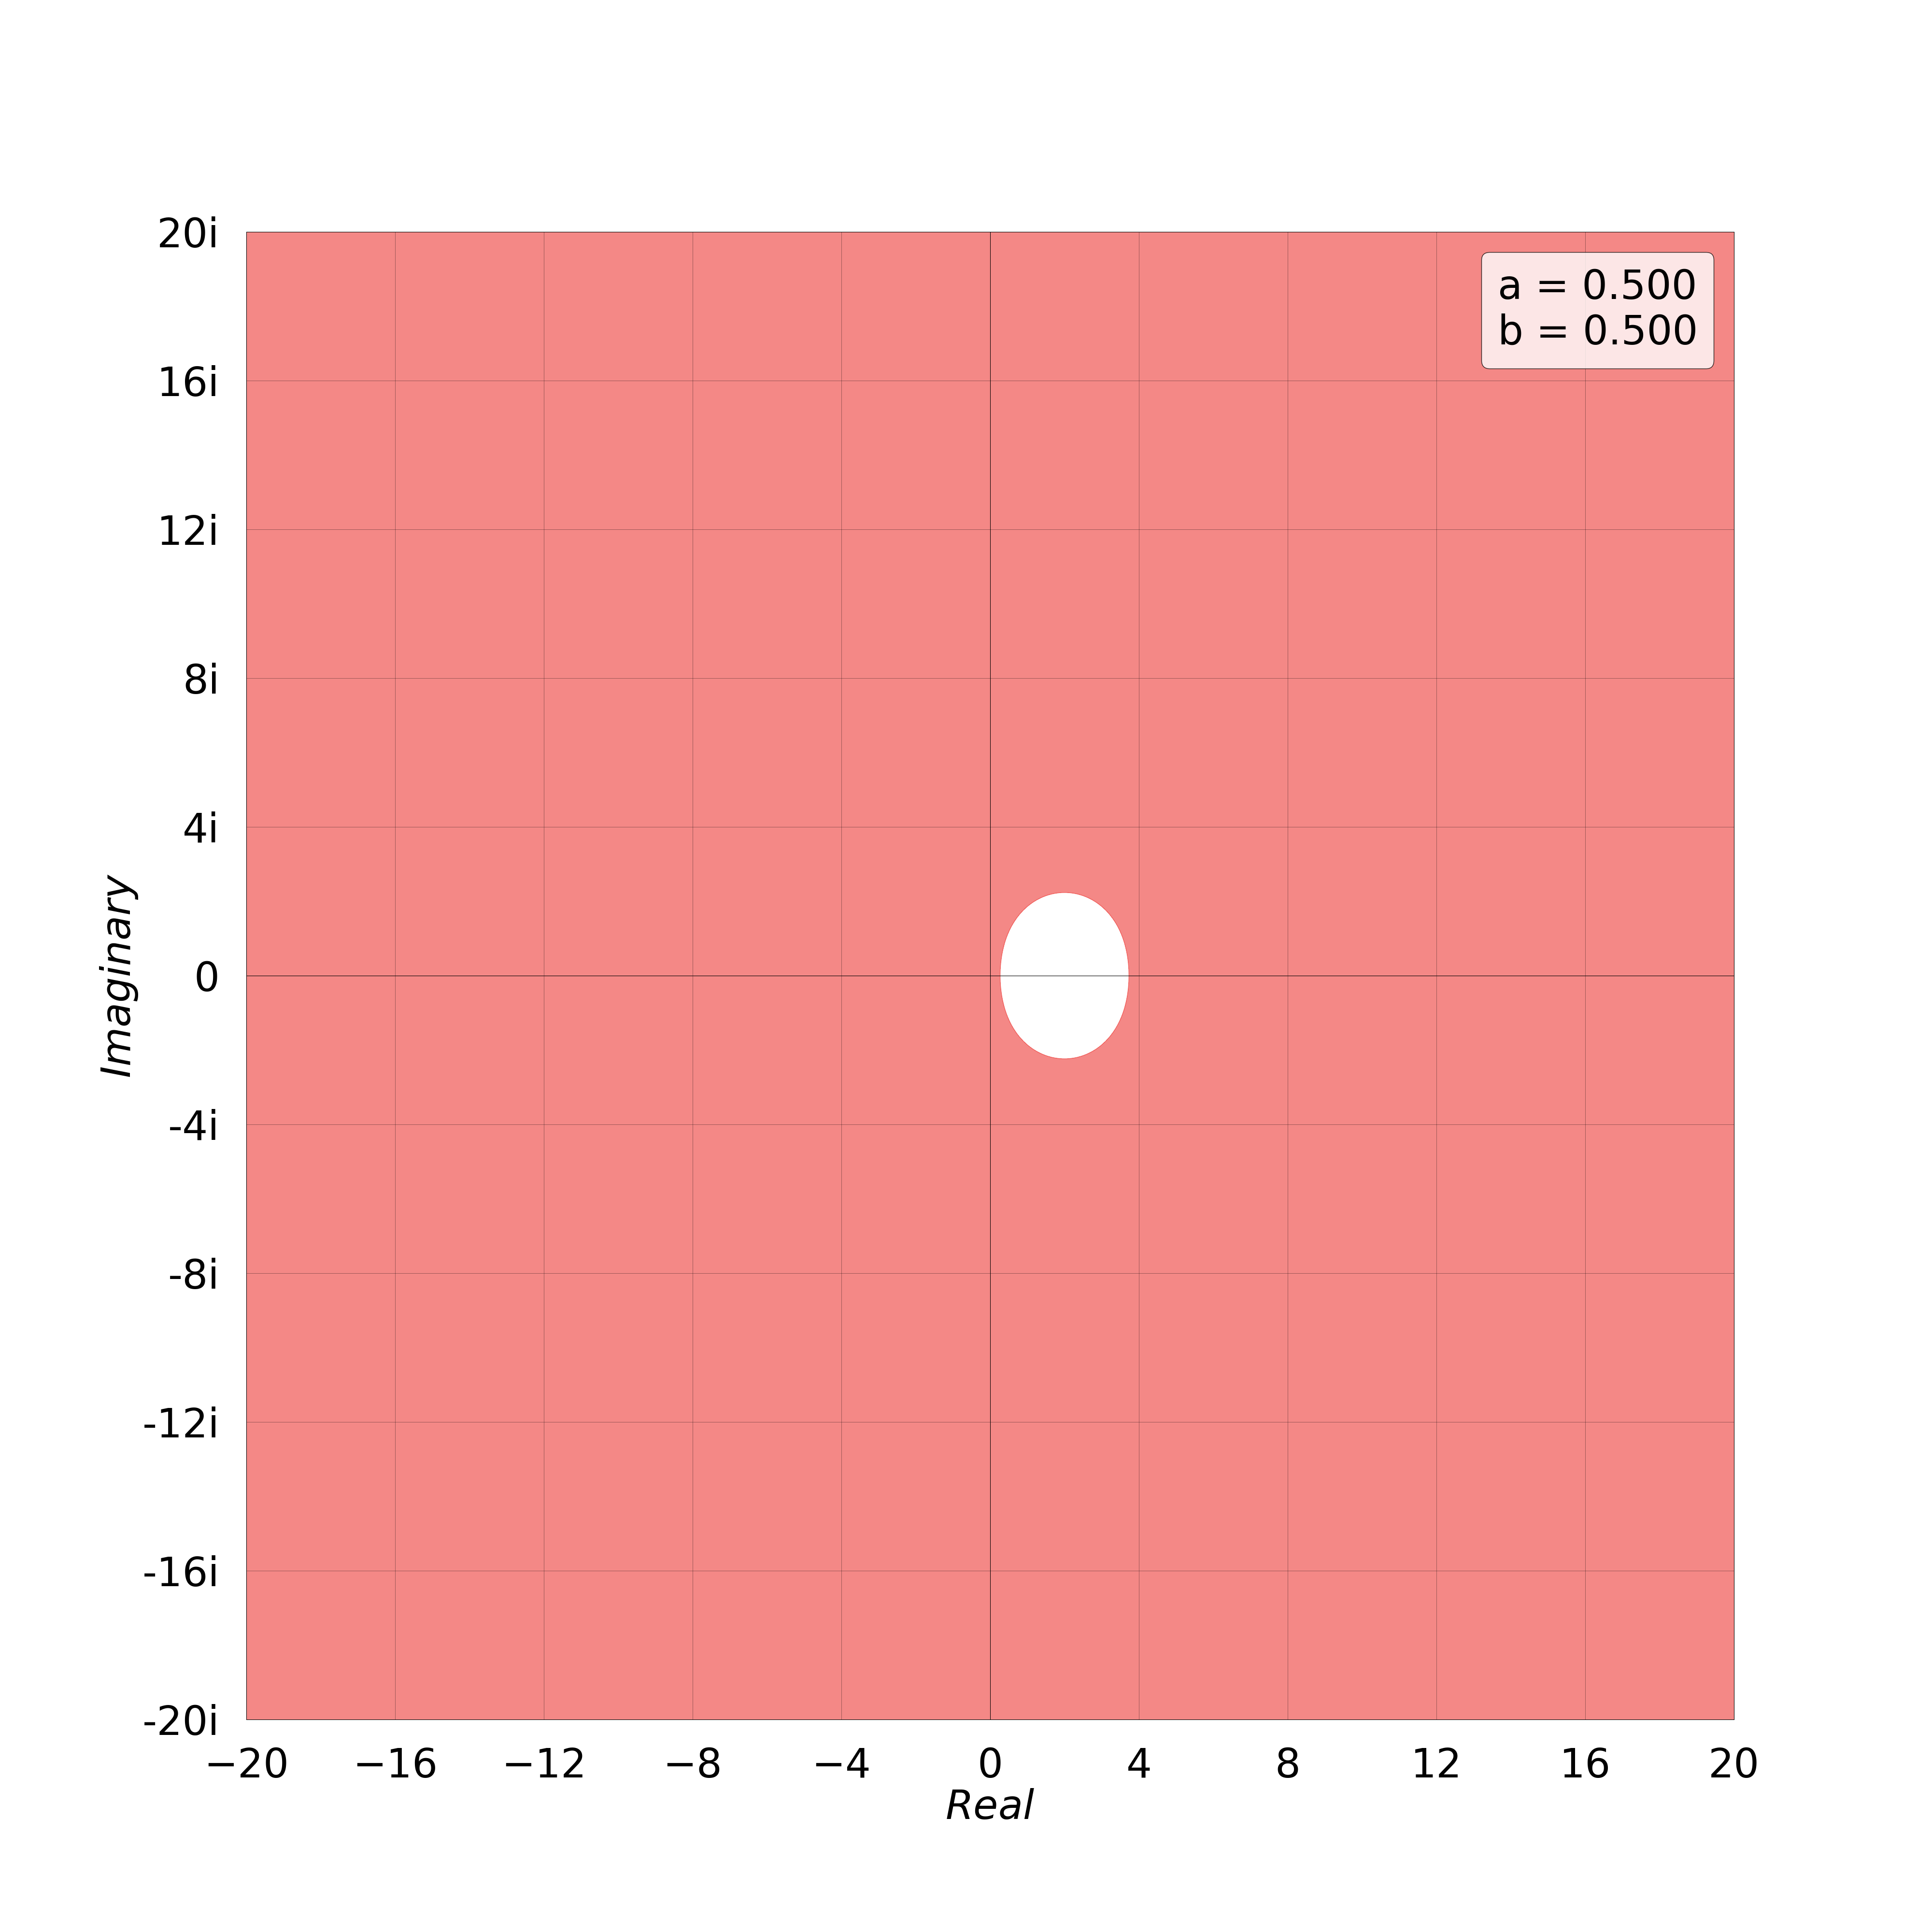
\includegraphics[width=0.32\textwidth]{Stability Regions/Videos/Varied a/Euler's Backward/b=0.5/frames/0500.png}
	\end{center}
	\columnbreak{}
	\begin{center}
		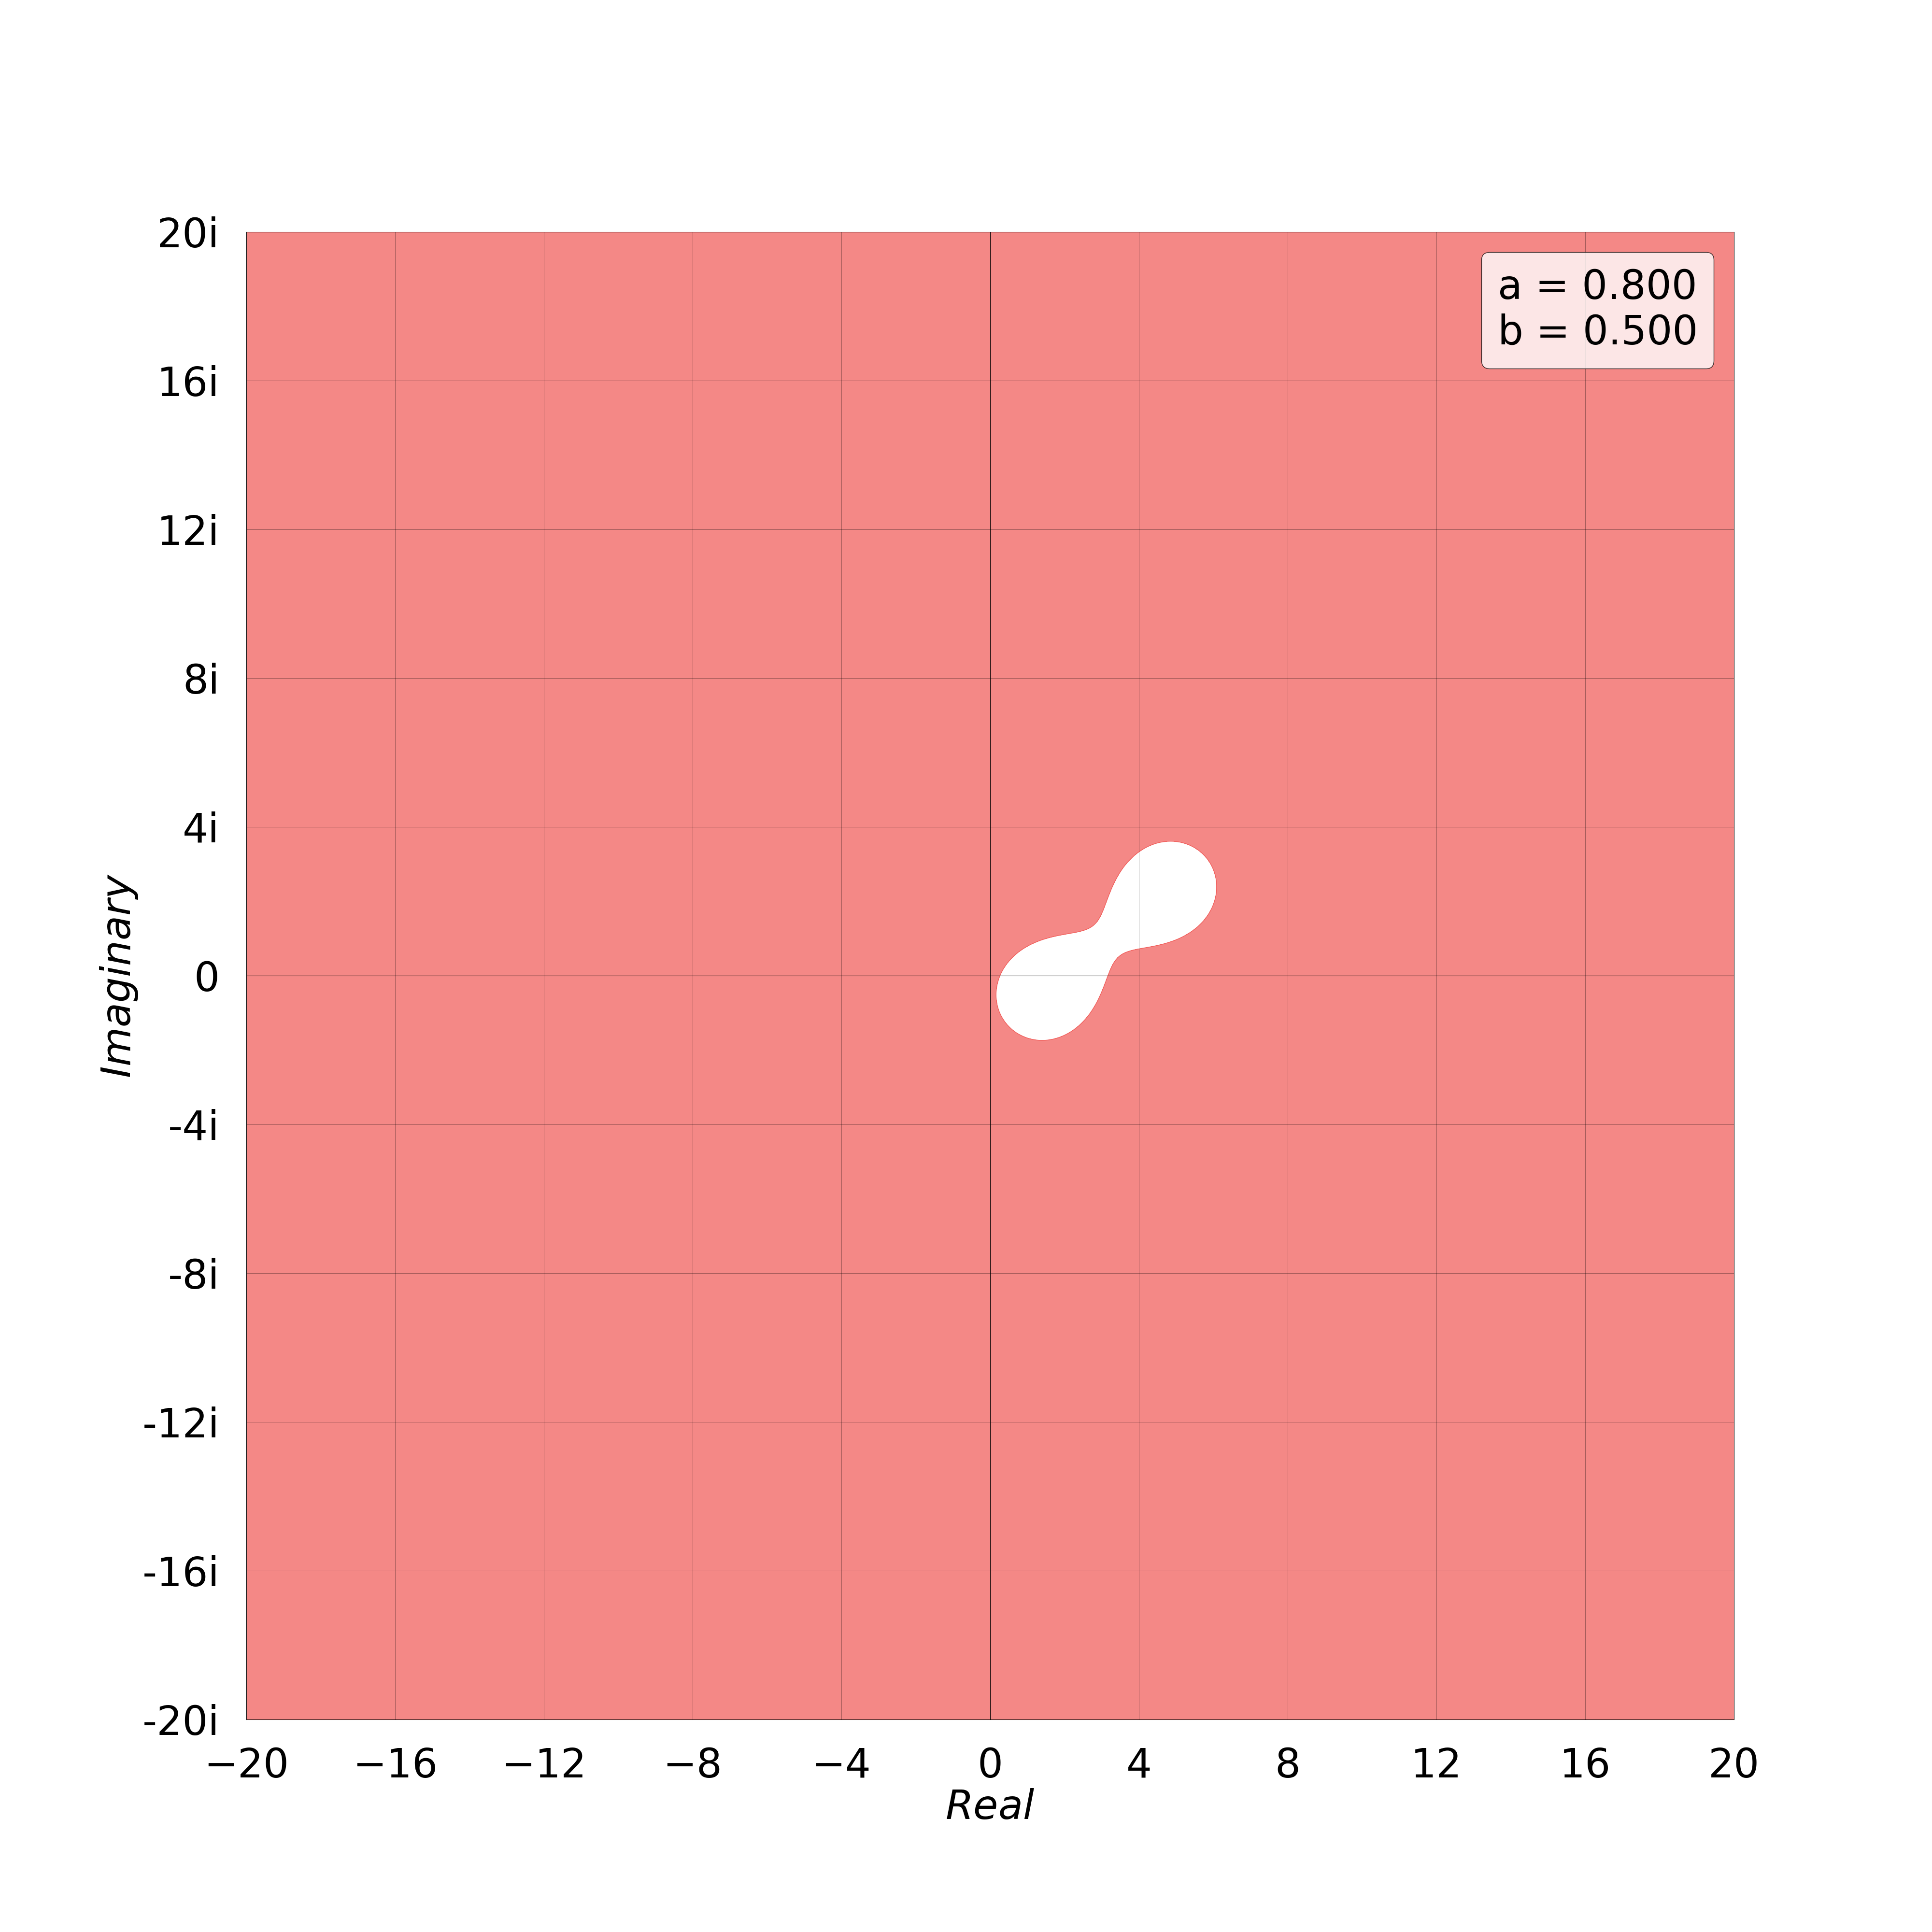
\includegraphics[width=0.32\textwidth]{Stability Regions/Videos/Varied a/Euler's Backward/b=0.5/frames/0800.png}
	\end{center}
\end{multicols}
\subsubsection{Runga-Kutta 4}
\vspace*{-0.65cm}
\begin{multicols}{3}
	\begin{center}
		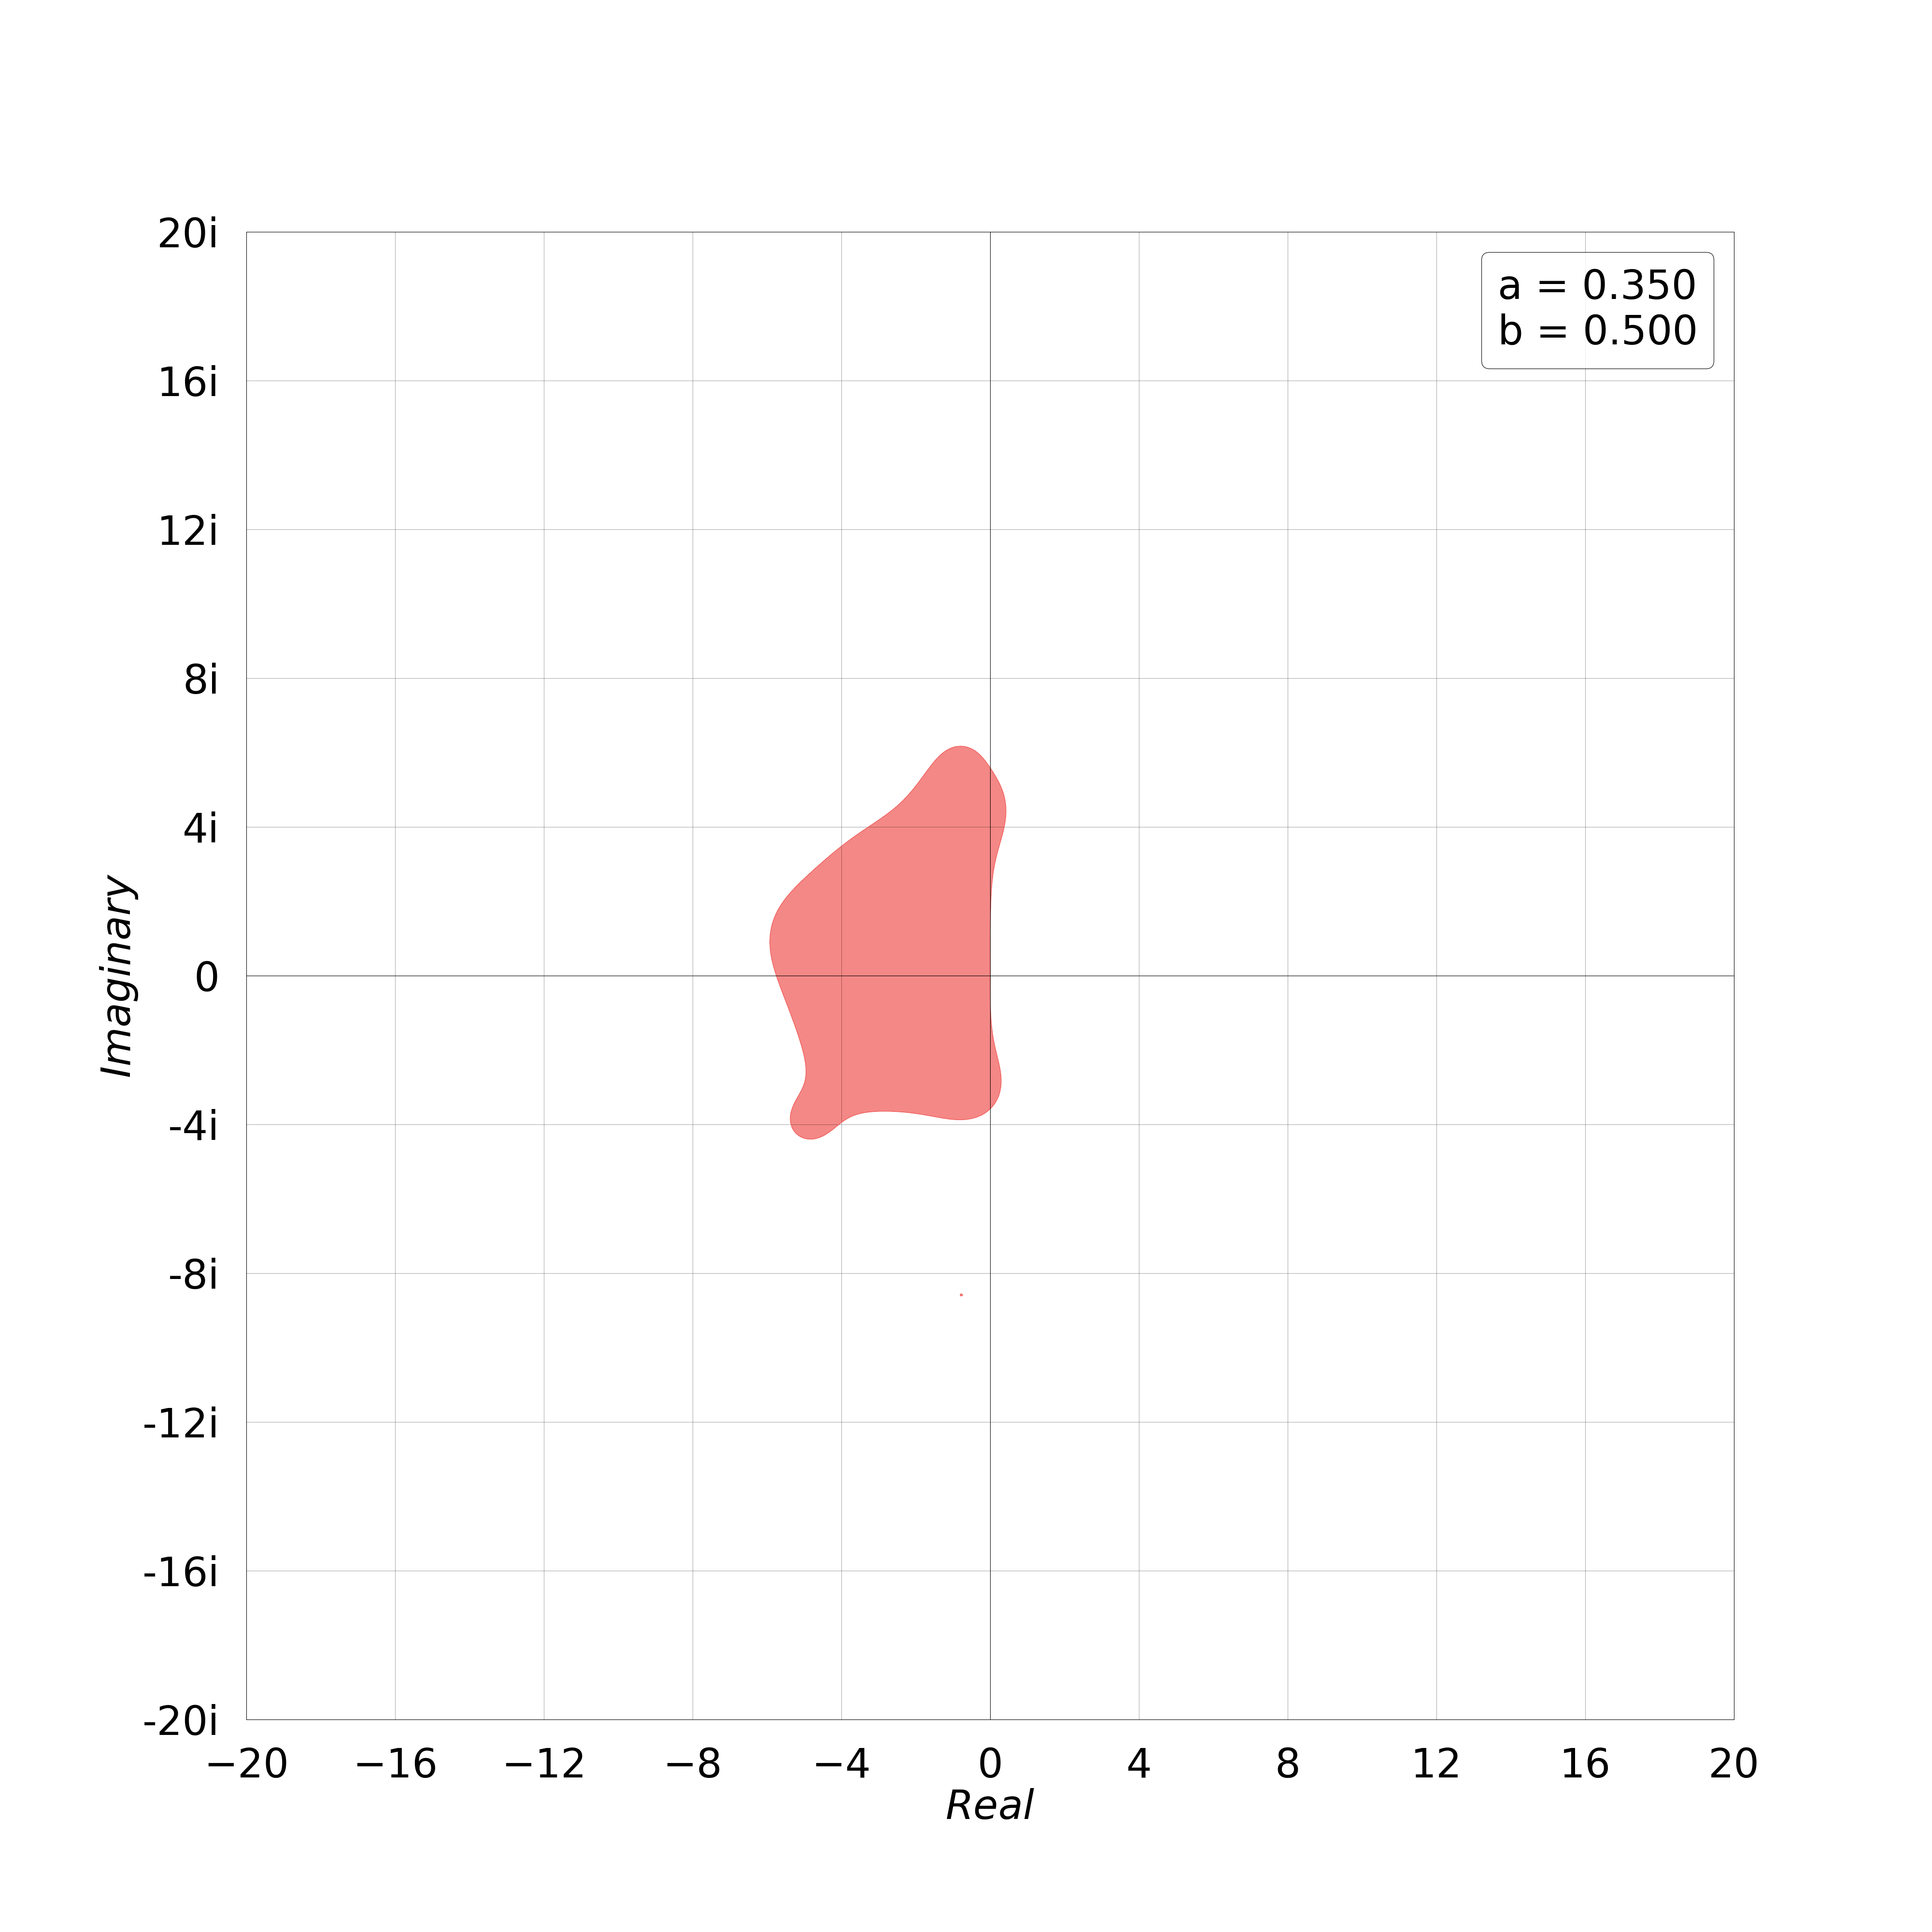
\includegraphics[width=0.32\textwidth]{Stability Regions/Videos/Varied a/Runge-Kutta 4/b=0.5/frames/0350.png}
	\end{center}
	\columnbreak{}
	\begin{center}
		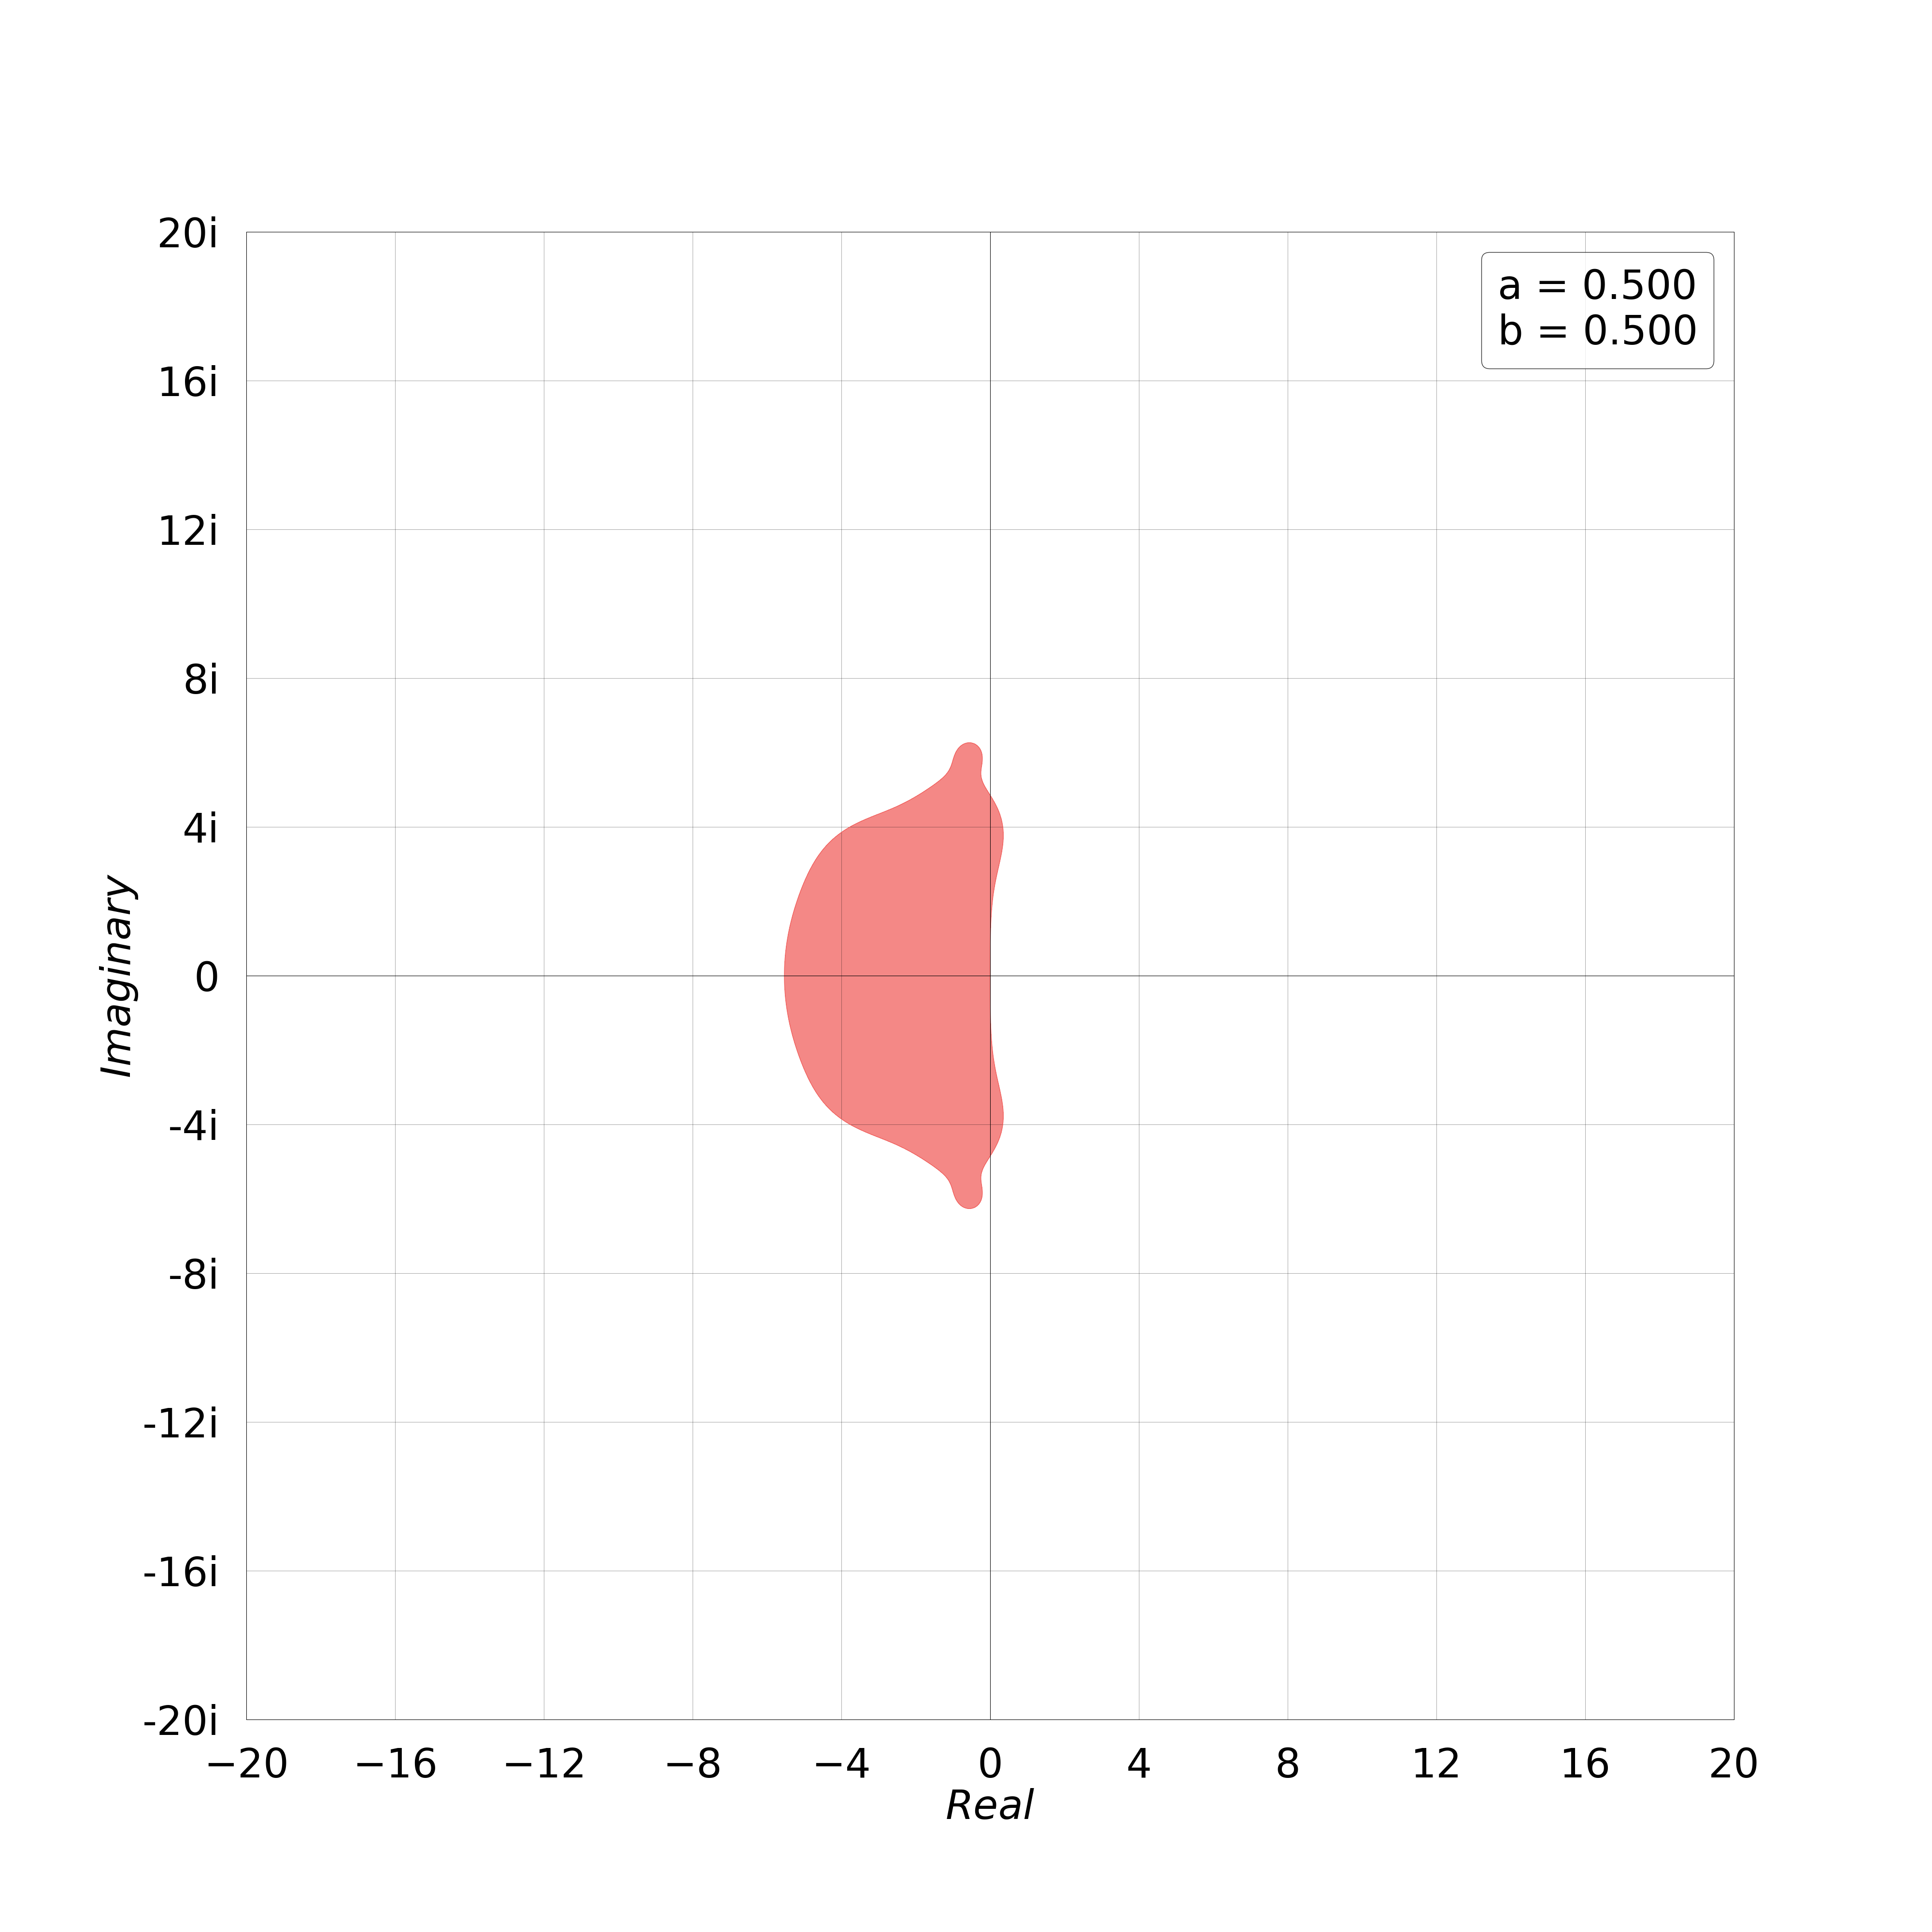
\includegraphics[width=0.32\textwidth]{Stability Regions/Videos/Varied a/Runge-Kutta 4/b=0.5/frames/0500.png}
	\end{center}
	\columnbreak{}
	\begin{center}
		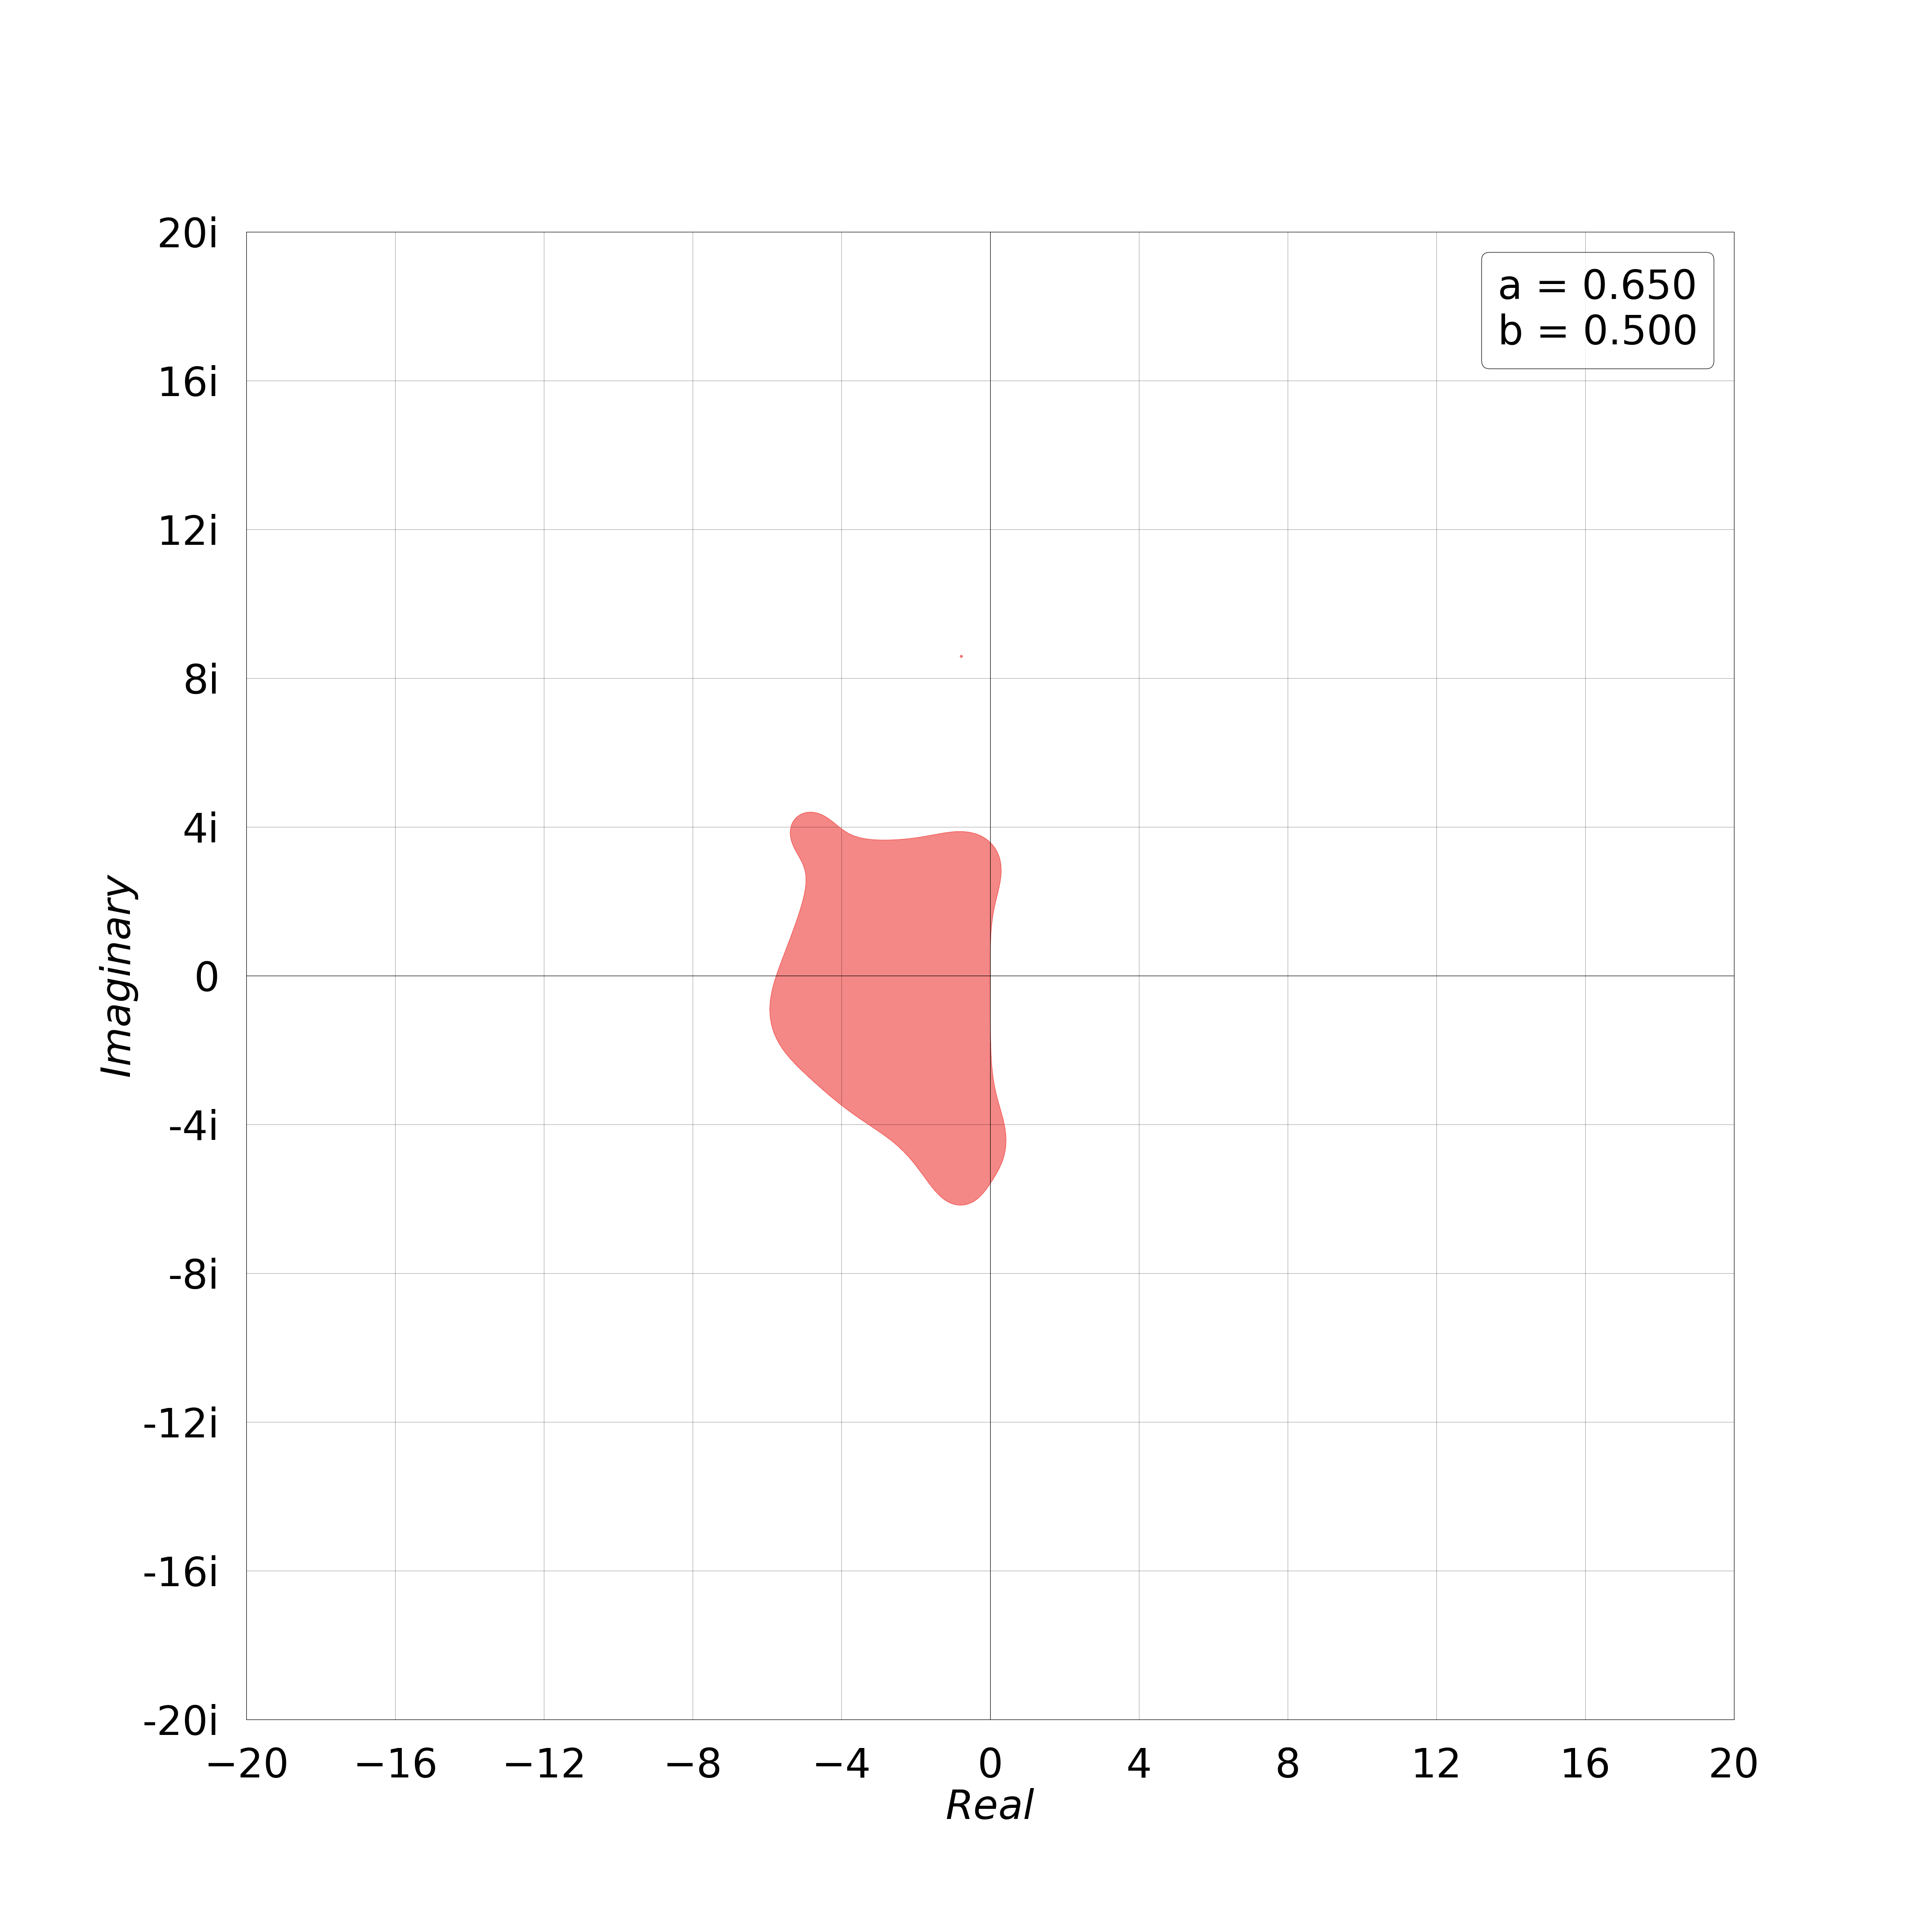
\includegraphics[width=0.32\textwidth]{Stability Regions/Videos/Varied a/Runge-Kutta 4/b=0.5/frames/0650.png}
	\end{center}
\end{multicols}

\newpage
\providecommand{\bysame}{\leavevmode\hbox to3em{\hrulefill}\thinspace}
\providecommand{\href}[2]{#2}
\begin{thebibliography}{1}

\bibitem{trefethen_definition}
Llyod N. Trefethen, \emph{{T}he definition of numerical analysis}, Cornell University, 1992.

\bibitem{walking_into_the_complex_domain}
Jithin D. George, Samuel Y. Jung, and Niall M. Mangan, \emph{{W}alking into the complex plane to `order' better time integrators}, \url{https://arxiv.org/abs/2110.04402}, 2021.

\bibitem{next}
Next reference.

\end{thebibliography}
 % bibliography

\end{document}
